% !TeX root = These.tex
\ifdefined\included
\else
\documentclass[french, a4paper, 11pt, twoside, pdftex]{StyleThese}
\usepackage{iflang}
\usepackage{bibentry}



%\usepackage[sectionbib]{chapterbib}          % Cross-reference package (Natural BiB)
%\usepackage{natbib}                  % Put References at the end of each chapter
%\usepackage{bibunits}
% Do not put 'sectionbib' option here.
% Sectionbib option in 'natbib' will do.


\usepackage{fancyhdr}                    % Fancy Header and Footer

\usepackage[utf8]{inputenc}
\usepackage[T1]{fontenc}
\usepackage[french]{babel} %
\usepackage{lmodern} \normalfont %to load T1lmr.fd 
\DeclareFontShape{T1}{cmr}{b}{sc} { <-> ssub * cmr/bx/sc }{}
%\hyphenation{gar}

\usepackage{amsmath,amssymb}             % AMS Math
\usepackage{nicefrac}
\usepackage{siunitx}					%% Unites Math SI

\usepackage{blindtext}

\usepackage{datetime}

\usepackage{lipsum} 

\usepackage[inline]{enumitem}

\usepackage{hhline}
%\usepackage[left=1.5in,right=1.3in,top=1.1in,bottom=1.1in]{geometry}
\usepackage[left=1.5in,right=1.3in,top=1.1in,bottom=1.1in,includefoot,includehead,headheight=13.6pt]{geometry}

%%\renewcommand{\baselinestretch}{1.05}

%%%%%%%% Multi-figures avec sub-captions
\usepackage{caption}
\usepackage{subcaption}

% Table of contents for each chapter

\usepackage[nottoc, notlof, notlot]{tocbibind}
\usepackage[nohints]{minitoc}
\setcounter{minitocdepth}{2}
\mtcindent=15pt
% Use \minitoc where to put a table of contents

\usepackage{aecompl}

%% Package cosmetic meilleur layout du texte en jouant sur le spacing par caractères
\usepackage[activate={true,nocompatibility},final,tracking=true,kerning=true,factor=1100,stretch=10,shrink=10]{microtype}
\usepackage[absolute,overlay]{textpos} 
\setlength{\TPHorizModule}{\paperwidth}\setlength{\TPVertModule}{\paperheight}
\sloppy

%%%%%%%%%%% JOLIS TABLEAUX
\usepackage{tabularx}		%\usepackage{tabular}
\usepackage{longtable}
\usepackage{multirow}
\newcommand{\mc}{\multicolumn} 
\newcommand{\mr}[2]{\multirow{#1}{*}{#2}} 	\newcommand{\mrQ}{\multirow{-4}{*}}
\usepackage{booktabs}

\usepackage[usenames,dvipsnames]{xcolor} 

\makeatletter
\newcommand{\ccolor}[3][]{%
	\kern-\fboxsep
	\if\relax\detokenize{#1}\relax
	\expandafter\@firstoftwo
	\else
	\expandafter\@secondoftwo
	\fi
	{\colorbox{#2}}%
	{\colorbox[#1]{#2}}%
	{#3}\kern-\fboxsep
}
\makeatother

%%%%% Insertion graphiques format PGF
\usepackage{pgfplots}
\pgfplotsset{width=\linewidth, compat=1.16}%, compat=1.17}
\usepackage{adjustbox}          %%% PERMET DE LES RECADRER + FACILEMENT


%%%%%%%%%% Bullets de listes sans saut de ligne %%%%%%%%%%
\usepackage{xparse}

\ExplSyntaxOn%
\seq_new:N \l_local_enum_seq

\newcommand{\storethestuff}[1]{%
  \seq_set_from_clist:Nn \l_local_enum_seq {#1}%
}

\newcommand{\dotheenumstuff}{%
\int_zero:N \l_tmpa_int
\seq_map_inline:Nn \l_local_enum_seq {%
    \int_incr:N \l_tmpa_int% Increase the counter
    \item ##1
    % Check whether the list has reached the end -- if so, use '.' instead of ','
    %\int_compare:nNnTF 
    % { \l_tmpa_int } < {\seq_count:N \l_local_enum_seq} 
    % {,} {.}
  }
}
\ExplSyntaxOff

\NewDocumentCommand{\linebullets}{+m}{%
  \storethestuff{#1}%
  \begin{enumerate*}[label={\alph*)},font={\bfseries},itemjoin={{, }}]
    \dotheenumstuff%
  \end{enumerate*}
}

\newcommand{\cmnt}[1]{}  %%%%% AJOUT DE COMMENTAIRE MULTILIGNES


%%%%%%%%%% ECRITURE CARACTERES DANS UN CERCLE %%%%%%%%%%
%\def\circleTxt[#1]{\raisebox{.5pt}{\textcircled{\raisebox{-1pt}{#1}}}}
\newcommand{\ctxt}[1]{\raisebox{.5pt}{\textcircled{\raisebox{-1.2pt}{#1}}}}
% Glossary / list of abbreviations

\usepackage[intoc]{nomencl}
\IfLanguageName{english}{%
\renewcommand{\nomname}{Glossary}
}{ %
\renewcommand{\nomname}{Liste des Abréviations}
}

\makenomenclature

% My pdf code

\usepackage{ifpdf}

\ifpdf
  \usepackage[pdftex]{graphicx}
  \DeclareGraphicsExtensions{.pdf,PDF,.png,PNG,.jpg,JPG}
  \usepackage[pagebackref,hyperindex=true]{hyperref} %% use \autoref{} instead of Table~\ref{}.
  \usepackage{tikz}
  \usetikzlibrary{arrows,shapes,calc}
\else
  \usepackage{graphicx}
  \DeclareGraphicsExtensions{.ps,.eps}
  \usepackage[a4paper,dvipdfm,pagebackref,hyperindex=true]{hyperref}
\fi

\graphicspath{{.}{schemas/}{graphiques/}{tables/}}

%% nicer backref links. NOTE: The flag ThesisInEnglish is used to define the
% language in the back references. Read more about it in These.tex

\IfLanguageName{english}{
\renewcommand*{\backref}[1]{}
\renewcommand*{\backrefalt}[4]{%
\ifcase #1 %
(Not cited.)%
\or
(Cited in page~#2.)%
\else
(Cited in pages~#2.)%
\fi}
\renewcommand*{\backrefsep}{, }
\renewcommand*{\backreftwosep}{ and~}
\renewcommand*{\backreflastsep}{ and~}
}{
\renewcommand*{\backref}[1]{}
\renewcommand*{\backrefalt}[4]{%
\ifcase #1 %
(Non cité.)%
\or
(Cité en page~#2.)%
\else
(Cité en pages~#2.)%
\fi}
\renewcommand*{\backrefsep}{, }
\renewcommand*{\backreftwosep}{ et~}
\renewcommand*{\backreflastsep}{ et~}
}

% Links in pdf
\usepackage{color}
\definecolor{linkcol}{rgb}{0,0,0.4} 
\definecolor{citecol}{rgb}{0.5,0,0} 
\definecolor{linkcol}{rgb}{0,0,0} 
\definecolor{citecol}{rgb}{0,0,0}
% Change this to change the informations included in the pdf file

\hypersetup
{
bookmarksopen=true,
pdftitle="Prévention des fautes temporelles sur architectures multicœur pour les systèmes à criticité mixte",
pdfauthor="Daniel LOCHE", %auteur du document
pdfsubject="Thèse", %sujet du document
%pdftoolbar=false, %barre d'outils non visible
pdfmenubar=true, %barre de menu visible
pdfhighlight=/O, %effet d'un clic sur un lien hypertexte
colorlinks=true, %couleurs sur les liens hypertextes
pdfpagemode=UseNone, %aucun mode de page
%pdfpagelayout=DoublePage, %ouverture en simple page
pdffitwindow=true, %pages ouvertes entierement dans toute la fenetre
linkcolor=linkcol, %couleur des liens hypertextes internes
citecolor=citecol, %couleur des liens pour les citations
urlcolor=linkcol %couleur des liens pour les url
}

% definitions.
% -------------------

\setcounter{secnumdepth}{3}
\setcounter{tocdepth}{2}

% Some useful commands and shortcut for maths:  partial derivative and stuff

\newcommand{\pd}[2]{\frac{\partial #1}{\partial #2}}
\def\abs{\operatorname{abs}}
\def\argmax{\operatornamewithlimits{arg\,max}}
\def\argmin{\operatornamewithlimits{arg\,min}}
\def\diag{\operatorname{Diag}}
\newcommand{\eqRef}[1]{(\ref{#1})}
\newcommand{\nline}{\smallbreak\noindent}

\usepackage{rotating}                    % Sideways of figures & tables

% \usepackage{txfonts}                     % Public Times New Roman text & math font
  
%%% Fancy Header %%%%%%%%%%%%%%%%%%%%%%%%%%%%%%%%%%%%%%%%%%%%%%%%%%%%%%%%%%%%%%%%%%
% Fancy Header Style Options

\pagestyle{fancy}                       % Sets fancy header and footer
\fancyfoot{}                            % Delete current footer settings

%\renewcommand{\chaptermark}[1]{         % Lower Case Chapter marker style
%  \markboth{\chaptername\ \thechapter.\ #1}}{}} %

%\renewcommand{\sectionmark}[1]{         % Lower case Section marker style
%  \markright{\thesection.\ #1}}         %

\fancyhead[LE,RO]{\bfseries\thepage}    % Page number (boldface) in left on even
% pages and right on odd pages
\fancyhead[RE]{\bfseries\nouppercase{\leftmark}}      % Chapter in the right on even pages
\fancyhead[LO]{\bfseries\nouppercase{\rightmark}}     % Section in the left on odd pages

\let\headruleORIG\headrule
\renewcommand{\headrule}{\color{black} \headruleORIG}
\renewcommand{\headrulewidth}{1.0pt}
\usepackage{colortbl}
\arrayrulecolor{black}

\fancypagestyle{plain}{
  \fancyhead{}
  \fancyfoot{}
  \renewcommand{\headrulewidth}{0pt} %%%%%%%%%%%%%%%%%%%%%%%%%%%%%%%%%%%%%%%%%%%%%%%%%%%%%%%%%%%%%%%%%%%%%%%%%%%%%%%%%%%%%
}

%\usepackage{MyAlgorithm}
%\usepackage[noend]{MyAlgorithmic}
%\usepackage[ED=EDSYS-SystEmb, Ets=INP]{tlsflyleaf}

%%% Clear Header %%%%%%%%%%%%%%%%%%%%%%%%%%%%%%%%%%%%%%%%%%%%%%%%%%%%%%%%%%%%%%%%%%
% Clear Header Style on the Last Empty Odd pages
\makeatletter

\def\cleardoublepage{\clearpage\if@twoside \ifodd\c@page\else%
  \hbox{}%
  \thispagestyle{empty}%              % Empty header styles
  \newpage%
  \if@twocolumn\hbox{}\newpage\fi\fi\fi}

\makeatother
 
%%%%%%%%%%%%%%%%%%%%%%%%%%%%%%%%%%%%%%%%%%%%%%%%%%%%%%%%%%%%%%%%%%%%%%%%%%%%%%% 
% Prints your review date and 'Draft Version' (From Josullvn, CS, CMU)
\newcommand{\reviewtimetoday}[2]{\special{!userdict begin
    /bop-hook{gsave 20 710 translate 45 rotate 0.8 setgray
      /Times-Roman findfont 12 scalefont setfont 0 0   moveto (#1) show
      0 -12 moveto (#2) show grestore}def end}}
% You can turn on or off this option.
% \reviewtimetoday{\today}{Draft Version}
%%%%%%%%%%%%%%%%%%%%%%%%%%%%%%%%%%%%%%%%%%%%%%%%%%%%%%%%%%%%%%%%%%%%%%%%%%%%%%% 

\newenvironment{maxime}[1]
{
	\def\Arg{#1}
\vspace*{0cm}
\hfill
\begin{minipage}{0.6\textwidth}%
%\rule[0.5ex]{\textwidth}{0.1mm}\\%
\hrulefill $\:$ \\%$\:$ {\bf #1}\\
%\vspace*{-0.25cm}
\it 
}%
{%
	
\hrulefill $\:$ {\bf \Arg}
\vspace*{0.5cm}%
\end{minipage}
}

\let\minitocORIG\minitoc
\renewcommand{\minitoc}{\minitocORIG \vspace{1.5em}}

%\usepackage{slashbox}

\newenvironment{bulletList}%
{ \begin{list}%
	{$\bullet$}%
	{\setlength{\labelwidth}{25pt}%
	 \setlength{\leftmargin}{30pt}%
	 \setlength{\itemsep}{\parsep}}}%
{ \end{list} }


%%%%%%% Outils pour \comment \alert \add %%%%%
\usepackage{easyReview}
\usepackage{soulutf8} % for accented letters

\let\newalert\alert
\renewcommand{\alert}[1]{\textit{\newalert{#1}}}

%\usepackage[commandnameprefix=ifneeded]{changes} %% \chhighlight and \chcomment to avoid collision with easyReview
\renewcommand{\epsilon}{\varepsilon}

% centered page environment

\newenvironment{vcenterpage}
{\newpage\vspace*{\fill}\thispagestyle{empty}\renewcommand{\headrulewidth}{0pt}}
{\vspace*{\fill}}

\usepackage{tablefootnote}

%%%%%% MISE EN FORME CADRES DEFINITIONS/THEOREMES/LEMES %%%%%%%%%%
\usepackage{amsthm}  % for theoremstyle

\theoremstyle{plain} 
\newtheorem{theorem}{Théorème}[section]
\newtheorem{corollary}{Corolaire}[theorem]

%\theoremstyle{lemma}
%\newtheorem{lemma}[theorem]{Lemme}


\theoremstyle{definition}
\newtheorem{definition}[theorem]{Définition}


\cmnt{
	\usepackage{ntheorem} %\usepackage{amsthm}  % for theoremstyle
	%\usepackage{mdframed}
	\usepackage[most]{tcolorbox}
	
	\theoremstyle{plain} 
	\theoremindent20pt
	\theoremheaderfont{\normalfont\bfseries\hspace{-\theoremindent}}
	\newtheorem{theorem}{Théorème}[section]
	\newtheorem{corollary}{Corolaire}[theorem]
	
	\theoremstyle{plain}
	\newtheorem{lemma}[theorem]{Lemme}
	
	
	\tcolorboxenvironment{theorem}{
		blanker,
		breakable,
		before skip=\topsep,
		after skip=\topsep,
		borderline west={1pt}{10pt}{double, shorten <=12pt}
	}
	
	\theorembodyfont{\normalfont}
	\theoremindent20pt
	\theoremheaderfont{\normalfont\bfseries\hspace{-\theoremindent}}
	\newtheorem{definition}[theorem]{Définition}
	
	
	\tcolorboxenvironment{definition}{
		blanker,
		breakable,
		before skip=\topsep,
		after skip=\topsep,
		borderline west={1pt}{10pt}{shorten <=12pt}
	}
}

\cmnt{ 
	\begin{theorem}
		Ceci est un Théorème.
	\end{theorem} 
	
	\begin{corollary}
		Ceci est un Corollaire.
	\end{corollary}
	
	\begin{definition}
		Ceci est une Définition.
	\end{definition}
	
	\begin{lemma}
		Ceci est un Lemme.
	\end{lemma}
}

\def\UrlBigBreaks{\do\/\do-\do:}
\usepackage{url}

\sloppy
\begin{document}
\setcounter{chapter}{5} %% Numéro du chapitre précédent ;)
\dominitoc
\faketableofcontents
\fi

	\setlength{\belowcaptionskip}{-6pt}
	
\chapter{Implémentation, Résultats et Analyse} \label{chap:5_ImplementationCase}
\minitoc

%%%% INTRO %%%%
Nous avons jusqu'alors présenté notre contribution pour garantir le respect d'échéances temporelles ciblées sur des tâches critiques par le biais d'un mécanisme de surveillance et de contrôle. Suite à cela nous avons proposé deux protocoles expérimentaux qui permettent de caractériser un jeu de tâches de façon à constituer un cas de test expérimental d'une part et pour configurer le-dit mécanisme d'autre part. À présent nous proposons la mise en application de tous ces éléments, par l'utilisation d'un jeu de tâches issus d'une suite de benchmark, MiBench. L'objectif est de tester et caractériser le comportement de ce mécanisme de surveillance et de contrôle sur un cas de test. Cette mise en œuvre consiste à développer un framework de configuration et d'exécution d'un jeu de tâches sur une plateforme Linux grand-public qui intègre le mécanisme ainsi que des patchs pour s'approcher d'une plate-forme temps-réel. L'objectif de ce framework est de proposer un environnement expérimental de mesures comportementales du mécanisme sur un cas de test modulable. On présentera dans un premier temps la plateforme de développement matérielle et logicielle. Nous verrons dans un second temps les détails d'implémentation du mécanisme de contrôle sur cette plateforme et comment le benchmark MiBench a été exploité dans ce contexte en application du protocole expérimental détaillé précédemment.

\newpage
\section{Plateforme de développement}
    
        \subsection{Plateforme Matérielle}
        	Le premier élément décisionnel repose sur le choix de la plateforme matérielle. Dans ce cadre-là, nous avons choisi une machine grand-public, un \textit{barebone PC} basé sur un processeur Intel Core i5-8250U. Il s'agit d'un processeur à quatre cœurs, qui peuvent fonctionner à une fréquence allant de 1600~MHz à 3400~MHz. Tel qu'on peut le visualiser sur le schéma d'architecture de ce processeur en~\autoref{fig:inteli58250Udie}, il dispose d'une mémoire locale partagée en la présence du cache L3 de 8~Mio\footnote{\textbf{Mébioctet -- }1 Mio = 2\up{20} octets = 1\,048\,576 octets, étant très proche de 1\,Mo = 10\up{9} octets = 1\,000\,000 octets, cette dernière unité est souvent utilisée à la place par simplification.}. Par ailleurs, chaque cœur dispose de deux niveaux de cache individuels, L1 et L2 qui peuvent respectivement stocker 32~Kio/cœur et 256~Kio/cœur. 
       	\begin{figure}[ht]
       		\centering
       		\includegraphics[width=0.8\linewidth]{kaby_lake_soc_block_annoted} %%
       		\caption{Circuit Intégré annoté de l'Intel i5 8250U}
       		\label{fig:inteli58250Udie}
       	\end{figure}
       
        	Sur ce type d'architecture, de nombreux points de contention peuvent provoquer des interférences entre les tâches. Dans la version schématisée du processeur en figure~\autoref{fig:kabylakesocblockdiagram}, une partie de ces éléments de contentions sont mis en valeur. On notera notamment le cache partagé ainsi que tous les bus de transfert de donnée (le "ring"), et les différents contrôleurs d'accès aux divers éléments. La problématique de la cohérence du cache a pu être étudiée en détail notamment dans~\cite{sensfelder_modeling_2019} ou encore \cite{boniol_identification_2019} pour les multicœurs COTS\footnote{COTS -- Commercial Off-The-Shell ou "Composant sur Étagère" désigne les produits disponible dans le commerce sans avoir été conçus pour un besoin spécifique.}.
        	
		\begin{figure}[ht]
			\centering
			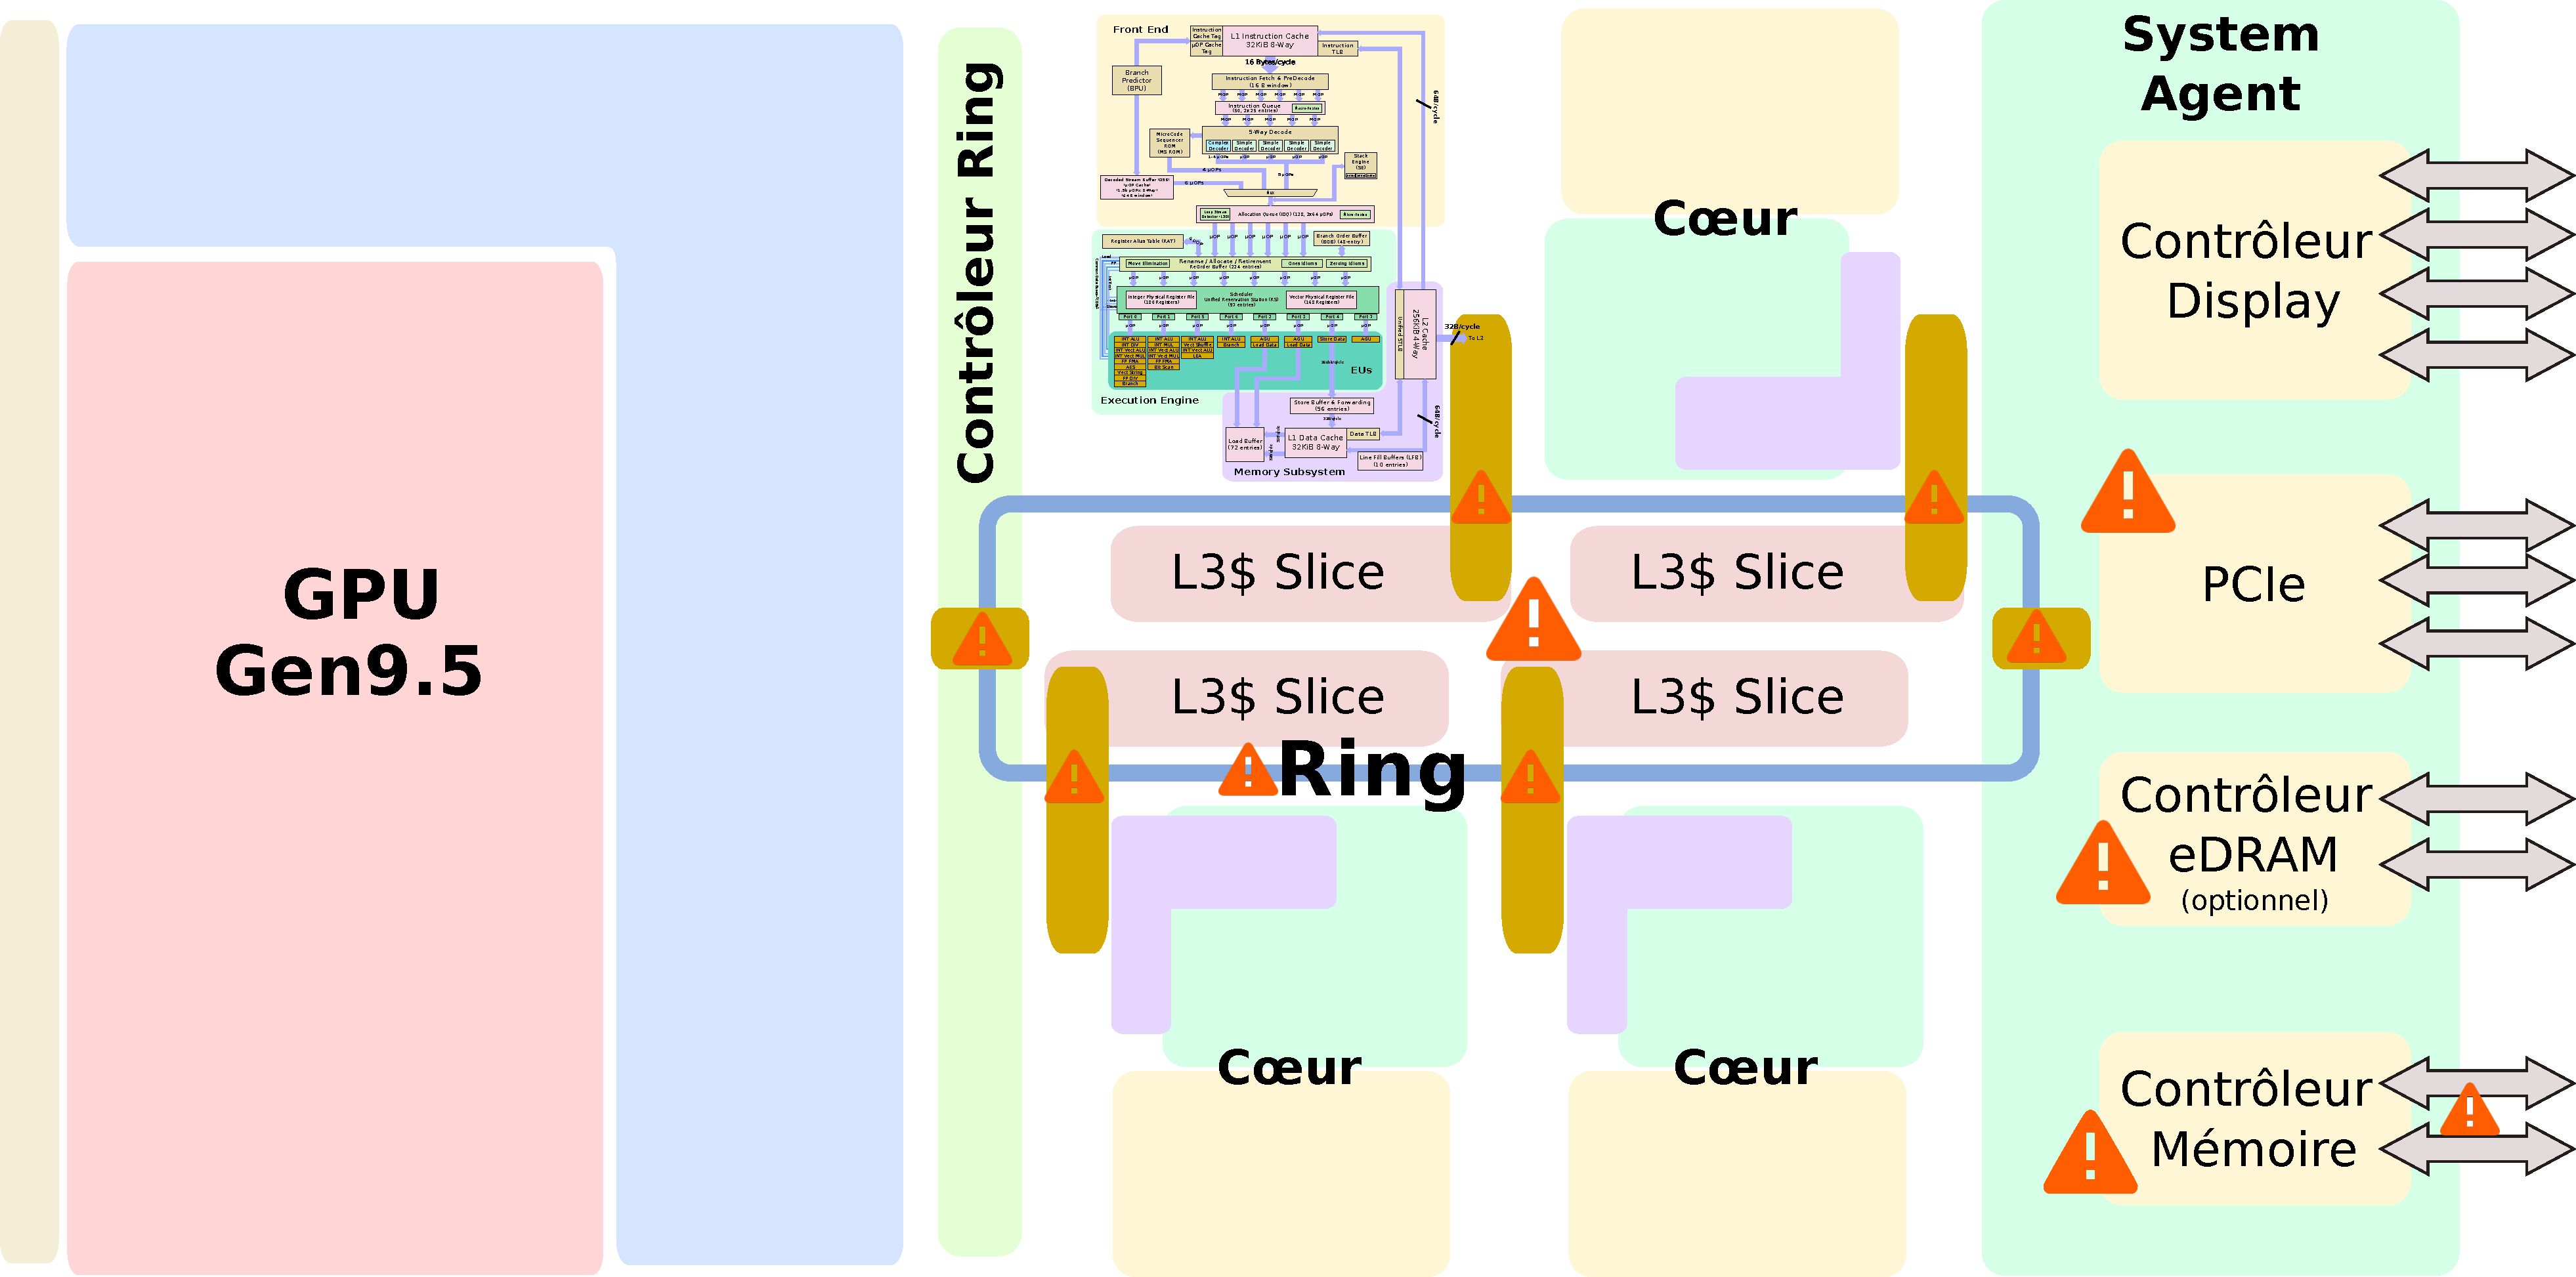
\includegraphics[width=\linewidth]{schemas/kaby_lake_soc_block_diagram}
			\captionsetup{justification=centering}
			\caption[Schéma de processeur multicœur avec points d'interférence]
					{Représentation schématique du processeur avec les points d'interférences notables}
			\label{fig:kabylakesocblockdiagram}
		\end{figure}
	
		Dans le cadre de nos expérimentations, nous établissons la fréquence de fonctionnement du processeur à une valeur fixe de 1600 MHz. L'hyperthreading est désactivé. Il s'agit d'une technologie permettant l'exécution parallèle de code sur un même cœur par dédoublement virtuel de ce dernier. Cela fait passer  le CPU de 4 cœurs physiques à 8 cœurs virtuels aux yeux du système d'exploitation. Son usage complexifie d'autant plus la gestion de l'utilisation de ressources partagées, et provoque même des partages de ressources supplémentaires, et par conséquent des sources d'interférence et donc de ralentissements d'exécution potentiels. Cela rend la maîtrise de l'exécution logicielle encore plus difficile par un mécanisme de contrôle et notamment pour obtenir une caractérisation représentative des interférences entre les tâches. De fait, cela nécessiterait d'observer toutes les possibilités d'exécution parallèle de code relatives à l'hyperthreading, en plus de toutes les possibilités d'exécution déjà existantes. Par conséquent, dans le cadre de notre étude et de façon plus générale, il nous semble plus pertinent de réaliser une implémentation sans utiliser de telles technologies, quitte à voir dans un second temps si leur ajout est envisageable.
		
		Avec notre seule proposition, de nombreuses possibilités supplémentaires sont offertes en comparaison des pratiques industrielles actuelles. De ces dernières, l'on pourra citer la désactivation complète du cache qui est une pratique courante pour éviter complètement tout effet de bord non prévu par l'intégrateur du logiciel, ou encore l'usage de stratégies d'ordonnancement statiques avec des fenêtres d'exécution temporelle fixes, et potentiellement surévaluées. Ces deux éléments représentent des limitations très importantes de performance des calculateurs émergents. Ces bridages nécessaires actuellement de par un manque de maîtrise du comportement matériel, pourraient être évités avec l'utilisation de mécanismes de contrôle dynamique comme le nôtre. 
		
		Au regard de ce constat, il convient donc de réaliser ces études de façon progressive et donc de ne pas impliquer directement la totalité des mécanismes d'optimisation mis à disposition par les processeurs, qui apportent chacun une couche de complexité supplémentaire.
		
		%\pagebreak
        \subsection{Support Logiciel}
        
        \paragraph{Système d'exploitation Linux --}
        Pour mettre en application nos bancs d'essais sur cette plateforme matérielle, nous avons cherché à reprendre un système d'exploitation qui permette le plus de versatilité possible via l'utilisation d'un système Linux. L'intérêt est double. 
        
        D'une part cela offre l'opportunité de tester une grande variété de logiciels et donc de pouvoir réadapter la solution à d'autres cas et contextes d'application. Cette richesse de logiciel se traduit aussi par l'existence de librairies déjà mises à disposition et éprouvées pour nos différents besoins. On pourra mentionner la capacité de gestion de l'ordonnancement et de l'exécution des tâches, l'automatisation des tests par scripts, des outils de stress du matériel ou encore de benchmarking (\cite{king_stress-ng_2019}) et monitoring du logiciel comme avec~\cite{girbal_metrics_2018}. Par ailleurs, plusieurs travaux ont déjà été effectués sur l'étude de Linux dans le cadre d'usage pour des systèmes temps-réel, tel que~\cite{litayem_building_2011}, \cite{allende_towards_2019} ou encore \cite{serra_architecture_2020}. Ainsi, ce type de système d'exploitation est déjà largement utilisé pour des cas d'application comme en robotique~\cite{bouchier_embedded_2013} ou sur des plateformes de prototypage automobile~\cite{sivakumar_automotive_2020}, \cite{gobillot_esprit_2018}.
        
        D'autre part, l'utilisation d'une plateforme matérielle et logicielle Linux apporte un niveau de complexité supplémentaire vis-à-vis de plateformes industrielles COTS qui emploient un micro-kernel. Cela se traduit particulièrement sur la politique d'ordonnancement et de gestion des tâches dans Linux comme cela a pu être couvert dans~\cite{lozi_linux_2016}. Cela présente un intérêt particulier. En effet, en obtenant des résultats probants sur l'efficacité d'un mécanisme de surveillance et de contrôle dans un environnement où l'on ne maîtrise pas totalement les couches bas niveau du logiciel alors on sera en droit d'être optimistes pour des cas d'utilisation sur des supports logiciels plus maîtrisés. La différence principale étant de soumettre un test sur une distribution Linux grand public qui implique déjà un certain nombre de tâches et de drivers qui s'exécutent en fond, qui n'ont pas été pensés pour du temps réel, plutôt que d'embarquer uniquement le logiciel dédié et contrôlé d'un cas réel.
        
        Nous nous baserons plus spécifiquement sur une distribution Linux Mint XFCE, version 20.04, avec un noyau en version 4.15.8.
        
        \paragraph{Co-noyau Xenomai --}
        De façon à utiliser Linux dans le cadre d'applications temps-réel, nous y adjoignons Xenomai~\cite{gerum_xenomai_2004} en version 3.1. Il s'agit d'un co-noyau qui se patche au noyau de base Linux de façon à lui apporter des fonctionnalités propres au développement d'applications temps-réel. Cela apporte notamment de meilleures performances en termes de latence comparé aux appels système Linux natif. Cela est dû au fait qu'initialement, le noyau Linux présente une grande part de code qui est non-préemptif. En conséquence, l'exécution de code non critique peut retarder la gestion d'interruptions destinées à exécuter du code temps-réel. Les différentes solutions de modification du noyau comme Xenomai, ou encore le patch \texttt{preempt-rt} dans une moindre mesure, répondent directement à cette problématique pour diminuer au mieux la latence constatée. Les écarts de latence observés sur la gestion des interruptions de l'ordre de millisecondes sont réduites à des microsecondes avec Xenomai. Les différentes solutions qui modifient Linux pour tenter d'y apporter un meilleur cadre d'utilisation de logiciel temps-réel ont pu être comparés dans~\cite{brown_how_2010}. 
        
        Le choix que nous avons fait a été déterminé aussi du fait qu'il fournit un framework complet pour exécuter des tâches temps-réel avec une gestion de tous les outils relatifs au domaine : \begin{itemize}
        	\item sémaphores et mutex,
        	\item d'envoi/réception de messages: pile, buffer, queues,
        	\item ordonnancement et allocation de tâches avec périodicité,
        	\item gestion d'alarmes et interruptions,
        	\item gestion d'entrée/sortie en évitant des latences propres à Linux.\end{itemize}
    	De plus, ce framework est disponible suivant différentes interfaces de développement. Cela facilite la portabilité d'une application entre différents frameworks temps-réel et le framework Xenomai natif. Ainsi, il est possible d'exécuter sur un support Xenomai du logiciel utilisant les interfaces de POSIX, PSOS, RTAI (qui est le prédécesseur de Xenomai), \textmu-ltron, VRTX, VxWorks et rtdm avec peu de modification du logiciel. Par ailleurs, notre choix de cette combinaison d'une carte mère basée sur un processeur Intel avec Xenomai est confortée par le fait qu'Intel ait déjà étudié la question de l'usage de Xenomai sur ses calculateurs multicœur~\cite{intel_corporation_hard_2009}. Ce framework sera utilisé pour l'implémentation du mécanisme de surveillance et contrôle.
    	
    	De façon générale, ce qui permet à Xenomai d'offrir toutes ces fonctionnalités avec des latences réduites en cohabitation avec le noyau Linux réside dans l'ajout d'une couche \texttt{Adeos}~\cite{gerum_life_2005} qui est un pipeline des  interruptions. Il permet la préemption de toutes les interruptions système pour les distribuer en priorité vers le domaine Xenomai avant tout envoi de ces dernières vers le domaine Linux. Cela inclut à la fois les interruptions matérielles et logicielles, ainsi que tous les envois de signaux système (changement d'état d'une tâche pour la mettre en pause/démarrer/arrêter, gestion de mutex etc.). Cela priorise \textit{de facto} l'exécution de code du domaine Xenomai et réduit au maximum les latences dues au noyau Linux. La différence entre un noyau Linux simple et avec un patch Xenomai est représenté en ~\autoref{fig:architecturekernel}. On constate que le co-noyau propose un équivalent symétrique aux composants natifs du noyau Linux, il s'agit en effet de répliquer en grande partie ce qui est mis à disposition dans le noyau Linux. À la différence d'être directement prévu pour limiter au maximum les latences d'exécution tout en ajoutant les couches nécessaires de compatibilité.

  	
		Il est à noter qu'au sein des systèmes Linux, ce que l'on nomme "\textit{tâche}" est désigné sous le nom de processus ou de thread. La différence fondamentale entre ces deux appellations étant que chaque processus possède son propre espace mémoire virtuel, tandis que les threads peuvent se partagent un espace mémoire virtuel commun s'ils sont lancés à partir d'un même processus parent. Du point de vue de l'ordonnancement du système d'exploitation, threads et processus sont équivalents. Cette différence sur la mémoire est, en ce qui nous concerne, négligeable. En effet, il s'agit bien de mémoire \textit{virtuelle}, c'est-à-dire que du point de vue des processus ils disposent d'un espace mémoire réservé, mais dans les faits il s'agit de mémoire physique qui est partagée. Le contrôleur mémoire du système d'exploitation étant responsable de la mise en correspondance entre adresses mémoires virtuelles et espaces mémoires physiques. Ainsi, que l'on travaille avec des threads ou des processus, les risques d'interférences par usage de ressources partagées tel que les cache reste identique. On continuera à parler de "tâches" par la suite.
	
	\begin{figure}[ht]
		\centering
		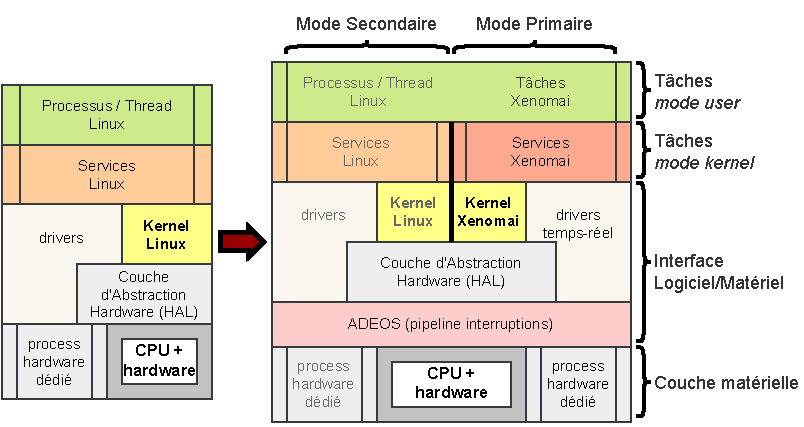
\includegraphics[width=\linewidth]{schemas/Architecture_kernel}
		\caption[Architecture co-noyau Linux et Xenomai]{Architecture du noyau Linux et Linux avec co-noyau Xenomai}
		\label{fig:architecturekernel}
	\end{figure}
	
		Il existe deux modes d'exécution des tâches sur un système Linux~:  en mode User ou Noyau, que l'on peut retrouver sur les 2 couches supérieures de l'architecture logicielle de la~\autoref{fig:architecturekernel}. Dans le mode Noyau, les tâches ont les droits pour exécuter des instructions privilégiées. Cette distinction est importante, car les opérations bas niveau que nous devons employer pour la surveillance et la gestion d'ordonnancement des tâches nécessite l'emploi d'instructions privilégiées. Avec l'utilisation de Xenomai s'ajoute une nouvelle dimension. Les tâches peuvent alors s'exécuter soit dans le domaine Xenomai en \textit{mode Primaire}, soit dans le domaine Linux en \textit{mode Secondaire}. L'avantage principal du domaine Xenomai étant la faible latence d'exécution, proche d'un système temps-réel dur. En revanche si une tâche dans ce domaine requiert des appels système Linux, alors une migration vers le domaine Linux est nécessaire. Xenomai réalise cela par un mécanisme de \textit{shadowing} où la tâche est clonée dans le domaine Linux en mode Secondaire pour effectuer les appels systèmes nécessaires. La transition entre les modes se fait de façon "fainéante" (\textit{lazy mode switch}) dans le sens où un changement de mode n'est fait qu'au moment où un appel de fonction requiert d'être dans l'autre mode de fonctionnement.
		
		Si nous relevons cette spécificité logicielle, c'est parce que chaque changement de mode engendre un surcoût de temps d'exécution avec le clonage de la tâche. Par conséquent, une tâche qui utiliserait successivement des appels système Linux et des fonctionnalités Xenomai bas-niveau peut très vite engendrer un très fort surcoût d'exécution. Parmi les fonctionnalités de Xenomai on peut citer par exemple la gestion de mutex, de signaux ou autres appels aux APIs temps-réel de Xenomai (gestion d'ordonnancement, alarme, interruptions...). C'est d'ailleurs pour cette raison qu'au fil du temps un bon nombre d'appels système ont eu droit à leur équivalent dans les API de Xenomai, pour éviter un passage en mode secondaire. C'est le cas par exemple des fonctions d'écriture dans la sortie standard \texttt{printf()} qui devient \texttt{rt\_printf()}. De façon plus générale, la correspondance entre les différents domaines applicatifs de Xenomai est un aspect très important de son développement pour permettre le plus facilement possible une inter-compatibilité entre les différents systèmes temps-réel et Linux. Une bonne part des enjeux et des méthodes déployées pour l'implémentation d'un système temps-réel donné sous Linux est développé dans~\cite{gerum_xenomai_2015}. 
	    Dans le cadre de l'utilisation d'un jeu de tâches arbitraire pour la réalisation de nos tests, nous devons être vigilants sur l'utilisation d'appels système et du nombre de changements de mode. Des tâches ayant de mauvais résultats sur ces métriques (notamment un surplus de changement de modes) sont probablement inadaptées à représenter des tâches temps-réel, à moins d'être modifiées spécifiquement pour éviter ce problème. 
		\smallbreak
		
        En résumé, par le biais de ce support logiciel, il est possible d'exécuter un ensemble de tâches donné, sous forme de processus séparés. Pour chacun d'entre eux la stratégie d'ordonnancement employée, le niveau de priorité, ainsi que l'allocation de la tâche sont configurables. L'allocation indique au système d'exploitation quels sont les cœurs qui sont autorisés à exécuter une tâche, autrement dit, à quels cœurs elle est allouée. C'est ce qui permet de déterminer pour chaque tâche si elle subira un ordonnancement partitionné (allocation à un unique cœur) ou global (allocation à tous les cœurs, par défaut).  Ainsi, pour un système à 4 cœurs par exemple, chaque tâche $\tau$ sera associée à une table d'affinité $A(\tau) = \begin{pmatrix}1 & 1 & 1 & 1\end{pmatrix}$ par défaut, signifiant qu'elle peut être exécutée sur n'importe lequel des 4 cœurs. Cette liberté rend notamment service à l'ordonnanceur pour équilibrer la charge entre les cœurs. Pour notre cas, et quand il s'agit d'exécuter une application temps-réel, il est intéressant d'exploiter ce mécanisme d'affinité. De cette façon, il sera possible d'isoler des tâches critiques sur un cœur par exemple, et d'appliquer une politique semi-partitionnée (si les tâches non critiques ne sont pas allouées à des cœurs spécifiques), voire complètement partitionnée (si les tâches non critiques sont toutes aussi allouées à des cœurs spécifiques).
        
        Et à propos d'ordonnancement sous Linux (et donc par extension, avec Xenomai), il s'établit selon un schéma assez spécifique~\cite{ishkov_complete_2015}. Il s'agit d'un ordonnancement global, mais qui prend en ligne de compte les 3 éléments susmentionnés dans l'ordre suivant~:
        \begin{itemize}
        	\item l'allocation de la tâche,
        	\item le niveau de priorité,
        	\item la stratégie d'ordonnancement.
        \end{itemize}
    	En effet, il s'agit en premier lieu d'un ordonnanceur par niveau de priorités. Pour les tâches classiques exécutées par Linux, ce niveau de priorité est dynamique, selon le temps déjà donné à chaque tâche par le processeur. Il s'agit de l'ordonnancement \textit{Completely Fair Scheduling} (CFS)~\cite{wong_towards_2008}, \cite{pabla_completely_2009}. En revanche, quand il s'agit de tâches à plus haut niveau de priorité (labellisées \texttt{RT} par le gestionnaire de tâches), où cette priorité est fixe, alors il existe plusieurs stratégies d'ordonnancement possibles. L'ordonnanceur sélectionne les tâches en attente d'abord par niveau de priorité décroissant. Puis les tâches d'un même niveau de priorité sont alors traitées selon leur politique individuelle. On a notamment First-In First-Out (FIFO), Rond-Robin (RR) et Earliest Deadline First (EDF\footnote{g-EDF pour être exact, disponible par patch~\cite{lelli_efficient_2011}. Linux ne gère pas une allocation partitionnée d'une tâche ordonnancée par EDF.}). Ceci étant dit, il est difficile de trancher de façon certaine sur la réaction de l'ordonnanceur en cas de coexistence de tâches de même niveau de priorité, mais avec plusieurs stratégies d'ordonnancement différentes...
    	Ainsi, si l'on souhaite par exemple tester un système à priorité fixe on pourra laisser la stratégie d'ordonnancement par défaut et modifier uniquement les niveaux de priorité. Pour un système en round-robin, il faudra positionner toutes les tâches au même niveau de priorité, toutes avec l'ordonnancement RR.

   %Therefore, we add a Xenomai co-kernel to improve latency down to micro-seconds and run our MCA to respect desired real-time constraints.
                        
    \section{Logiciel Applicatif}
        \subsection{Benchmark MiBench}
        \paragraph{Présentation --} MiBench est un benchmark qui a été développé par Guthaus \& al.~\cite{guthaus_mibench_2001} dans l'idée de proposer une librairie d'applications qui couvrent un large panel de domaines. Nous l'utilisons de façon à pouvoir en sélectionner des tâches pour représenter au mieux un cas d'application réaliste. 
        Ce benchmark dispose de codes source ainsi que de données type qui sont utilisables pour lancer chaque application. Aussi, elles sont toutes disponibles en deux versions, "petite" et "grande" qui, comme cela le laisse penser, implique des temps d'exécution ou une empreinte mémoire (selon l'application) plus ou moins conséquente. Cela se fait soit par l'utilisation d'un code différent volontairement plus complexe et plus demandeur en ressources de calcul, soit par la modification des données d'entrée/sortie pour prévoir des plus grandes tailles de données (quand il s'agit d'un traitement d'image par exemple). Au total, ce sont 30 tâches, chacune en version "petite" et "grande" donc. Le résumé des tâches de ce benchmark est présenté dans la~\autoref{tab:mibench_tasks} .

\setlength{\tabcolsep}{4pt}    
\begin{longtable}{@{}llll@{}}
%	\centering
	\caption{Tâches MiBench}\label{tab:mibench_tasks} \\
%	\begin{tabular}{@{}llll@{}}
		\toprule
		Nom          & Description                                  & Type d'entrée      & Type de sortie         \\ \midrule
	\endfirsthead
		\multicolumn{4}{c}{\tablename\ \thetable\ -- Tâches MiBench (suite)}\\[1ex]
		\toprule
		Nom          & Description                                  & Type d'entrée      & Type de sortie         \\ \midrule
	\endhead
		\bottomrule 
	\endfoot
		basicmath	 & calculs scientifiques				& /					 & données (dec.)	\\
		bitcount     & comptage de bits	vers entiers        & texte ASCII        & texte ASCII      \\
		qsort        & algorithme de tri                    & texte ASCII        & texte ASCII      \\
		susan c      & reconnaissance de coins              & image (.pgm)       & image (.pgm)     \\
		susan e      & reconnaissance de bords              & image (.pgm)       & image (.pgm)     \\
		susan s      & lissage d'image (réduction de bruit) & image (.pgm)       & image (.pgm)     \\
		jpeg c       & encodeur JPEG                        & image (.ppm)       & image (.jpeg)    \\
		jpeg d       & décodeur JPEG                        & image (.jpeg)      & image (.ppm)     \\
		lame         & encodeur MP3                         & audio (.wave)      & audio (.mp3)     \\
		mad          & décodeur audio MP3                   & audio (.mp3)       & audio (.wave)    \\
		tiff2bw      & conversion en noir et blanc          & image (.tiff)      & image (.tiff)    \\
		tiff2rgba    & conversion couleurs RGB en TIFF		& image (.tiff)      & image (.tiff)    \\
		tiffdither   & tramage noir et blanc (dithering)    & image (.tiff)      & image (.tiff)    \\
		tiffmedian   & réduction de plage de couleur      	& image (.tiff)      & image (.tiff)    \\
		dijkstra     & recherche de plus court chemin		& texte ASCII        & texte ASCII      \\
		patricia     & recherche sur arbre PATRICIA			& texte ASCII        & texte ASCII      \\
		ghostscript  & interpréteur PostScript              & PostScript		 & image (.ppm)     \\
		ispell       & Vérificateur orthographique          & texte              & texte ASCII		\\
		rsynth       & synthèse vocale de texte             & texte              & audio (.AU)      \\
		stringsearch & recherche de mot dans un texte		& texte              & texte            \\
		blowfish d   & déchiffrement blowfish               & données (bin.)  	 & données (bin.)   \\
		blowfish e   & chiffrement blowfish                 & texte              & données (bin.)   \\
		pgp d        & déchiffrement asymétrique      		& données (bin.)  	 & texte            \\
		pgp e        & chiffrement asymétrique				& texte              & données (bin.)   \\
		rijndael d   & déchiffrement AES                    & données (bin.)  	 & texte            \\
		rijndael e   & chiffrement AES                      & texte              & données (bin.)   \\
		sha          & algorithme de calcul de hash			& texte              & texte ASCII      \\
		adpcm c      & encodeur de PWM                      & audio (.wave)      & données (bin.)   \\
		adpcm d      & décodeur de PWM                      & données (bin.)  	 & données (bin.)   \\
		CRC32        & somme de contrôle 32 bits     		& audio (.wave)      & texte ASCII      \\
  	fft (fft\up{-1}) & transformée de fourrier (/inverse)	& signal (sinus)	 & signal (sinus)	\\ 
		gsm toast    & encodage GSM                         & audio (.AU)        & données (bin.)   \\ 
		gsm untoast  & decodage GSM                         & données (bin.)     & audio (.AU)	    \\ 		
%		\bottomrule
%	\end{tabular}
\end{longtable}
    
    
    Ces tâches sont classifiées en 6 domaines d'application~: automobile, réseau, utilisateur, bureautique, sécurité et télécoms. On retrouve ici la notion de criticité mixte qui nous intéresse pour la cohabitation de ces fonctionnalités au sein d'un même calculateur, car chaque domaine applicatif implique sans aucun doute des niveaux de criticité différents.
    Il faut cependant préciser que nous n'avons pas pu faire fonctionner toutes ces fonctions, à cause de difficultés de compilation difficilement surmontables de par la complexité du code impliqué notamment. Par conséquent, un premier tri de ces tâches s'effectue naturellement. 
    
 	\paragraph{Adaptation --} Aussi, il a fallu modifier le benchmark manuellement pour convenir à une utilisation en tant que librairie de notre framework. Les codes sources ont été modifiés un par un de deux façons~: 
	\begin{itemize}
		\item  	Uniformiser la méthode de récupération des données d'entrée de chaque application, de même pour la sortie. Toutes les tâches qui utilisaient des arguments d'entrée pour indiquer un fichier d'entrée à accéder en lecture, voire le fichier de sortie, ont été ajustées pour à la place utiliser l'entrée et sortie standard, modifiables avec la syntaxe shell (\texttt{<~[entrée]} et \texttt{>~[sortie]}). Les appels internes uniquement dédiés à du log de l'avancement ont aussi été retirés, typiquement l'usage de fonctions tel que \texttt{printf("Calcul en cours\textbackslash{}n");}.
		\item  	Proposer une fonction appelable depuis du code externe pour lancer un job de chaque tâche MiBench. Les codes sources et outils de compilations ont donc été adaptés pour être exploités en tant que librairies (compilation sans linkage), avec une fonction du nom de la tâche à la place des \texttt{main()}. Ainsi, le \texttt{main()} de la tâche fft par exemple, a été remplacé par une fonction \texttt{fft()} qui sera utilisable par notre framework.
	\end{itemize} Avec ces modifications, il a été possible de compiler chaque tâche en tant que fonction en librairie, qui sera reliée par la suite à notre framework expérimental pour être utilisée.

 	Le récapitulatif des tâches que nous avons pu exploiter à l'issue de tout cela, classées par domaines, est listé en~\autoref{tab:MiBench_final}. Des analyses comportementales de ces tâches ont déjà pu être réalisées par le passé, notamment par Blin \& Al.~\cite{blin_understanding_2016} sur la consommation mémoire et le profil d'accès mémoire/calculs/écriture mémoire de ces tâches. Ce type de données et les expérimentations réalisées pour les obtenir demeurent donc une source précieuse et complémentaire au protocole expérimental que nous proposons pour la caractérisation des tâches et la compréhension de leur rôle dans l'apparition d'interférences.
    
    \begin{table}[ht]
    	%% increase table row spacing, adjust to taste
    	%\renewcommand{\arraystretch}{1.3}
    	\caption{Tâches MiBench conservées}
    	\label{tab:MiBench_final}
    	\centering
    	\begin{tabular}{@{}ll@{}}
    		\toprule
    		Domaine		& Tâches					\\
    		\midrule
    		Automotive  & basicmath, bitcount, qsort, susan (smooth/edges/corners)	\\
    		Network     & dijkstra, patricia                                        \\
    		Consumer    & jpeg (décode/encode)		                            \\
    		Office      & stringsearch                                              \\
    		Security    & blowfish (décode/encode), rijndael (décode/encode), sha, CRC32		\\
    		Telecom     & adpcm (décode/encode), FFT, FFT\up{-1}, gsm (décode/encode)   \\
    		\bottomrule
    	\end{tabular}
    \end{table}
   % En amont de l'implémentation de ce benchmark à notre cas de test, il est important de préciser qu'il a fallu passer par une phase d'adaptation et de compilation dédiée. 

	\subsection{Charge de test}
	En complément du benchmark pour représenter la charge utile du système, il nous faut l'outillage nécessaire à l'application d'un stress du processeur pour obtenir les profils des tâches en pire cas tel que décrit dans le \hyperref[chap:4_ProtocolExpe]{Chapitre précédent}. À cette fin, nous utilisons deux éléments.
	
	D'une part la suite \texttt{Stress-ng}~\cite{king_stress-ng_2019} qui est un outil relativement complet et avancé pour stresser chaque partie du système de façon assez précise. Il est ainsi possible de lancer une charge artificielle forcée sur l'utilisation du CPU, sur le cache (avec même des effacements forcés du cache), la mémoire ou encore les entrées/sorties (communication réseau par exemple). Pour pousser le système dans des conditions de fonctionnement encombrées, nous utiliseront en particulier la commande suivante : 
		\begin{lstlisting}[numbers=none]
	stress-ng --ionice-class rt --cache 4    \
	          --fault 4 --io 4 --matrix 2\end{lstlisting}
	
	Si l'on regarde en détail cette commande, on identifie en premier lieu le passage en priorité haute avec \texttt{-{}-ionice-class rt} de façon à ce que le stress ne reste pas relégué à l'arrière plan best-effort. Ensuite, 4 éléments de stress distinct sont lancés : 
	\begin{description}
		\item \texttt{-{}-cache 4} -- Stress du cache via 4 processus,
		\item \texttt{-{}-fault 4} -- Stress de la mémoire (par provocation de \textit{page faults}),
		\item \texttt{-{}-io 4} -- Stress des entrées/sorties génériques,
		\item \texttt{-{}-matrix 2} -- Stress multi-éléments sur l'utilisation CPU, cache et mémoire par calculs matriciels avec virgule flottante via 2 processus.
	\end{description}

	En complément de cet outil, Xenomai propose aussi de quoi effectuer des stress avec la fonction \texttt{DoHell}. En revanche, les effets exacts de ce stress sur le système ne sont pas clairs, par manque de documentation. Par conséquent, nous pourrons employer les deux pour avoir une double soumission au stress de nos tâches. Nous pourrons donc de la même façon utiliser : 

	\begin{lstlisting}[language=bash, numbers=none]
	dohell -b -s 192.168.0.1 -m /tmp 800\end{lstlisting}
	
	
	Cette commande permet d'exécuter une charge spécifique avec l'option \texttt{-b}, en plus d'un fort trafic réseau avec \texttt{-s 192.168.0.1} et une charge de lecture/écriture mémoire avec \texttt{-m /tmp}, pendant 800 secondes.
        
    \subsection{Implémentation de la plateforme expérimentale logicielle}
    
    À partir de tous les éléments que nous venons de présenter, il est possible de mettre en place une plateforme expérimentale complète pour tester le mécanisme de surveillance et contrôle dans un environnement personnalisable. Une telle plateforme se caractérise par 3 grands leviers~: \begin{itemize}
    	\item le \textbf{support de développement}, tant matériel que logiciel que nous venons de présenter ;
    	\item les \textbf{hypothèses de modélisation}, que nous avons présentées au~\autoref{chap:3_PrincipeArchi}. Il s'agit du modèle de tâches à criticité duale et de chaîne de tâches ainsi que le modèle du mécanisme de surveillance et de contrôle étudié ;
    	\item les \textbf{paramètres d'entrée}, qui se composent d'une part du système logiciel auquel on applique les hypothèses de modélisation (en l’occurrence, les tâches MiBench) et d'autre part du paramétrage du mécanisme. Il s'agit donc des éléments présentés dans le~\autoref{chap:4_ProtocolExpe}.
    \end{itemize}
	L'ensemble de ces éléments sont agrégés dans la~\autoref{fig:expeOverview}. Cela permet de visualiser simplement les différents éléments d'entrée de la plateforme expérimentale, qui sont tout autant de vecteurs ajustables pour tester l'incidence des différents paramètres de la plateforme. 
	
	\begin{figure}[ht]
		\centering
		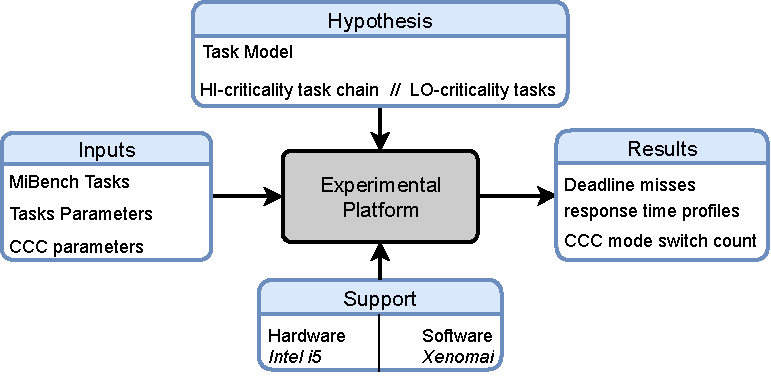
\includegraphics[width=0.9\linewidth]{ExperimentsArch}
		\caption{Structure générale de la plateforme expérimentale\label{fig:expeOverview}}
	\end{figure}

    	\subsubsection{Framework expérimental}
    
    La mise en place de cette plateforme expérimentale a débuté par la configuration, compilation puis installation d'un noyau Linux 4.15.8 patché avec un co-noyau Xenomai. Ensuite il a fallu mettre en place un framework générique de lancement de tests. Le framework en question répond aux objectifs suivants~:
    \begin{itemize}
    	\item récupérer une liste de tâches à exécuter avec leurs paramètres associés suivant un fichier de configuration,
    	\item lancer les tâches paramétrées, avec une encapsulation par le mécanisme de Surveillance,
    	\item lancer une tâche dédiée au mécanisme de Contrôle,
    	\item exécuter les tâches sur une durée déterminée puis sauvegarder toutes les traces d'exécutions dans un fichier de log.
    \end{itemize}

	Pour réaliser cela, on implémente un module \texttt{TaskLauncher} de configuration, qui prend en donnée d'entrée un fichier \texttt{conf.in} qui indique des groupes de tâches à lancer. 
	
	Ce groupement (plutôt que de lister directement toutes les tâches) permet de distinguer les tâches non critiques des tâches de la chaîne critique. Chaque ligne du fichier indique donc un groupe de tâches, avec un identifiant ID associé. ID = 0 pour des tâches non critiques, et ID $ \geq1 $ indique une chaîne critique et donc l'identifiant de la chaîne.
	En plus du niveau de criticité, il inclut la stratégie d'ordonnancement du groupe de tâches ainsi qu'un identifiant de groupe. S'il s'agit d'un groupe désignant une chaîne de tâches, l'échéance bout-en-bout est aussi indiquée. Un exemple de fichier de configuration est indiqué dans l'encadré de~\autoref{code:conf.in}.
	
\begin{lstlisting}[caption={Exemple type de fichier d'entrée conf.in}, label={code:conf.in}]
NAME         ID  PATH             DEADLINE (ms)  SCHED_POLICY
NonCritical   0  ./bestEffort.in     99999       BE
ComputeTraj   7  ./ComputeTraj.in      187       RM
	// ID = 0 : deadline value is unused.
\end{lstlisting}

	Aussi, chaque groupe dans ce fichier de configuration pointe vers des fichiers de configuration secondaires \texttt{tasks.in} qui donnent la liste de toutes les tâches de ce groupe à être exécutées avec les paramètres de chacune d'elles. Un exemple d'un tel fichier de configuration secondaire est donné en~\autoref{code:task.in}.
	%\pagebreak
	\begin{lstlisting}[caption={Fichier d'entrée pour une chaine de tâche}, label={code:task.in}]
ID name         rWCRT    T   P  A prec FUNC     ARGS
1  fft_S       129000   40  10  1   0  fft      8 2048 [...]
2  bitcount_S   93000   60  10  1   1  bitcnts  75000 [...]
3  basicmath_S  68000   40  10  1   2  bmath_S  > ./out/[...]
4  sha_S        49000   60  10  1   3  sha      < ./dat/[...]
5  fft_inv_S    25000   40  10  1   4  fft_i    8 4096 >[...]
6  gsmUToast_S  94000  100  10  1   5  utoast   -dfps -c [...]
7  fft_S        67500  100  10  1   6  fft      8 16384 >[...]
8  patricia_L       0  100  10  1   7  patricia < ./dat/[...]
// T=Period | P=Priority | A=Affinity | prec=Precedency
// rWCRT in us ; T in ms ; A in hexadecimal
\end{lstlisting} %//  prec = 0 : Tache entrante | rWCRT = 0 : Tache de sortie.
	
	Dans le détail, ces fichiers de paramètres des tâches comportent les éléments suivants, qui sont traités par le module \texttt{TaskManager}~: \qquad( [\textit{param.}] = \textit{optionnel} )
	\begin{description}
		\item \texttt{id} et \texttt{name} -- identifiant unique et nom de la tâche,
		\item \texttt{function} -- pointeur vers la fonction à réaliser (sous forme de librairie),
		\item \texttt{[arguments]} -- paramètres propres à la tâche et pointeur vers données d'entrée,
		\item \texttt{affinity} -- affinité, c.-à-d. les cœurs sur lesquels la tâche peut être exécutée,
		\item \texttt{periodicity} -- périodicité d'exécution des jobs (en millisecondes)
		\item \texttt{priority} -- niveau de priorité (si priorité fixe) (entre 0 et 100 sous Linux),
		\item \texttt{[precedency]} -- (si critique)~: tâche précédente dans la chaîne de tâches,
		\item \texttt{[rWCRT]} -- (si critique)~: paramètre de l'Agent de Contrôle $rWCRT(\tau_i)$ en {\textmu}s.
	\end{description}

    On peut remarquer 2 informations intéressantes dans le fichier de configuration d'une chaîne de tâche. D'abord à la ligne 2, la valeur de \texttt{prec = 0} pour désigner la tâche précédente. Cela indique de façon explicite qu'il s'agit de la tâche d'entrée de la chaîne. De la même façon, à la ligne 9, la valeur de pire temps de réponse restant \texttt{rWCRT = 0} indique qu'il s'agit de la tâche de sortie de la chaîne. 
    
     Les processus principaux de notre framework expérimental sont représentés avec leurs interactions en~\autoref{fig:implementationarchi}. Une fois les fichiers de configuration traités et interprétés par le \texttt{TaskManager}, ce dernier peut faire appel aux APIs Xenomai pour lancer toutes les tâches du système. Cela va donc inclure toutes les tâches décrites dans les fichiers de configuration, mais aussi une tâche dédiée à l'Agent de Surveillance et Contrôle. Une fois l'ensemble des tâches créées avec l'encapsulation des tâches et les canaux de communication dédiées au mécanisme de Surveillance, la totalité du système est lancé pour la durée fixée de l'expérimentation.
    
    \begin{figure}[ht]
    	\centering
    	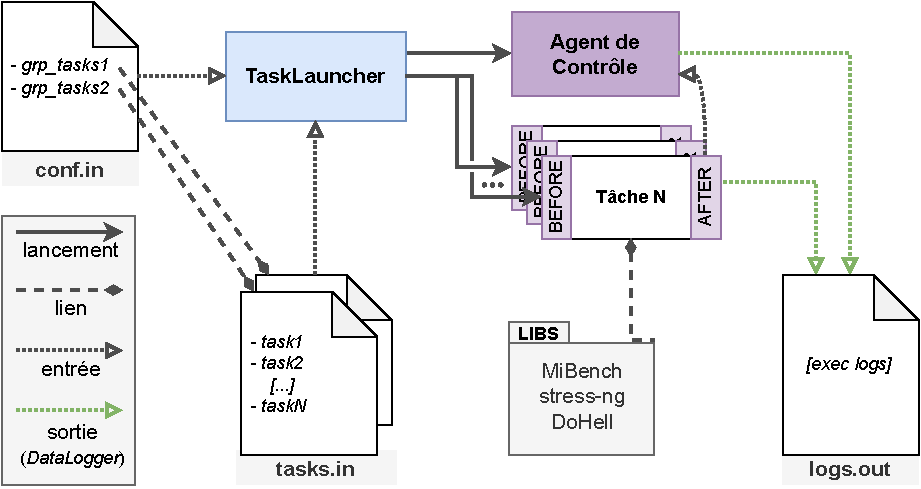
\includegraphics[width=\linewidth]{schemas/Implementation_Archi}
    	\caption{Fonctionnement du framework expérimental}
    	\label{fig:implementationarchi}
    \end{figure}

%\pagebreak 
    À la fin de l'expérimentation, le Mécanisme de Contrôle gèle l'exécution de l'ensemble de tâches et enregistre les profils d'exécution de la chaîne de tâche dans un fichier de sortie \texttt{logs.out}.  Enfin, grâce à un \texttt{DataLogger} ajouté dans l'encapsulation des tâches, chacune d'entre-t-elle enregistre aussi en sortie tous ses logs d'exécution. Ce module de log d'exécution, propre à notre plateforme expérimentale, est décorrélé du mécanisme de Surveillance et Contrôle. Il a été ajouté uniquement pour obtenir des mesures de début et fin d'exécution plus complètes (incluant les tâches non critiques), de façon à analyser plus en détail le comportement du système.
        
    	\subsubsection{Agent de Surveillance et Contrôle}

	L'agent de Surveillance et Contrôle que nous avons développé se décompose en 2 processus. 
	
	D'une part, le processus de \textbf{Surveillance} réceptionne les données de fin d'exécution des tâches critiques grâce à leur encapsulation et les stockent dans une mémoire tampon. Il s'exécute de façon évènementielle à chaque arrivée d'un nouveau timestamp. 
	
	D'autre part, un module de \textbf{Contrôle} consomme les données en mémoire tampon pour suivre exhaustivement l'état de la chaîne de tâches et permet le changement de mode. Ces deux processus correspondent ainsi aux deux blocs décrits dans le~\autoref{chap:3_PrincipeArchi} : Task Wrapper Component et Core Control Component.
	
	L’interaction entre les modules du Core Control Component et du Task Wrapper Component est illustré sur la~\autoref{fig:agentsurveillancecontrole}, avec la réception par évènement des timestamps de fin de tâches critiques et l'envoi de signal de passage en mode dégradé vers les tâches non critiques en cas d'anticipation.

	\begin{figure}[ht]
		\centering
		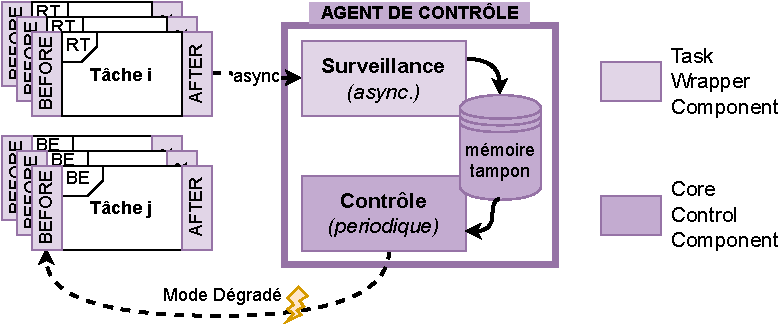
\includegraphics[width=0.8\linewidth]{schemas/AgentSurveillance_Controle}
		\caption{Interactions Agent de Surveillance-Contrôle avec les tâches}
		\label{fig:agentsurveillancecontrole}
	\end{figure}

	À la période $T_{CCC}$, le module de Contrôle traite les données en mémoire tampon. Pour se faire il conserve en mémoire les timestamps classées par tâches, de façon à pouvoir reconstruire l’État de la chaîne de tâches $S(t) = \left\langle t_0, \tau_p \right\rangle$ à partir de la date de début de la tâche entrante de la chaîne et par reconstruction de sa trace d'exécution jusqu'à l'instant t. Il peut alors calculer la condition \autoref{eq:safe_cond} - $ RT(t) + rWCRT(\tau_i) + W_{max} + t_{SW} \leq D_c $ pour anticiper une situation à risque qui demande un passage en mode dégradé. Le détail du fonctionnement interne du processus de Contrôle est représenté dans la \autoref{fig:algorithmecontrole}. On remarquera la nécessité des tables de stockage des timestamps des tâches $\tau_i$, de taille $L_i$, qui se remplissent à partir des éléments reçus par le TWC, et sont retirés à chaque complétion de la chaîne de tâche (tous les timestamps respectant les contraintes de précédence avec le timestamp de la tâche terminale sont délestés). 
	
	\begin{figure}[th]
		\centering
		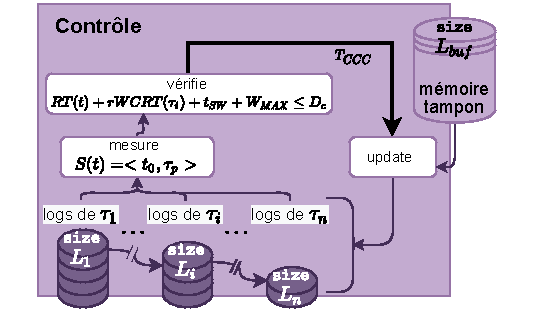
\includegraphics[width=0.7\linewidth]{schemas/Algorithme_Controle}
		\caption{Fonctionnement interne du Core Control Component}
		\label{fig:algorithmecontrole}
	\end{figure}
	
	Il est possible de définir les tailles minimales $L_i$ nécessaires des tables pour stocker les différents timestamps des tâches $\tau_i$ de la chaîne critique. Pour une tâche $\tau_i$, $i \in [\![1,n]\!]$ alors $L_i$ est fonction de la période d'activation et du nombre maximum possible d'instances actives de la chaîne de tâche à prendre en compte à un instant donné tel que défini au~\autoref{chap:3_PrincipeArchi} (Def.~\ref{def:EtatChaine}). Ainsi, avec $T_i$ et $C_i$ respectivement la période et le temps d'exécution pire cas de la tâche critique $\tau_i$, on a~: 
	\begin{equation}~\label{Cond:sizeBuffers}
		\forall~\tau_i, \  i \in [\![ 1, n ]\!],  \qquad L_i = \left\lceil \frac{\sum_{j=i}^{n}(C_j + T_j)-T_i}{T_i} \right\rceil
	\end{equation}

\pagebreak
	On notera que pour $i=n$, la tâche terminale, on trouve bien $L_n=1$ qui est logique cas dès qu'un job de la tâche terminale s'exécute, elle est directement délestée dans le mécanisme de Contrôle par la terminaison de l'exécution bout-en-bout correspondante. Il n'y aura donc jamais plus d'un timestamp de la tâche terminale de stockée, et il sera immédiatement retiré par définition des traces d'exécutions actives, qui sont les seuls conservées pour le suivi à un instant t.
	
%	\pagebreak
	
	Nous avons fait ce choix d'implémentation en deux composantes de façon à ce que la liaison entre l'Agent de Contrôle et les Wrappers se résume à un envoi de message, avec une tâche dédiée très simple qui a pour seul rôle de mettre ces messages en mémoire tampon pour être traités périodiquement par le CCC. Ainsi, une erreur dans l'envoi de ces messages ou dans leur réception n'empêche pas au module de Contrôle d'effectuer la vérification périodique. Cela évite aussi le partage de ressources entre les Wrappers et l'Agent de Contrôle. Et l'unique ressource partagée est interne à ce dernier, en la présence de la mémoire tampon. En conclusion, la modélisation de l'ensemble figure dans le diagramme de classe simplifié en~\autoref{fig:implementationdiagrammedeclasse}.
	
%	\pagebreak
	
	\begin{figure}[ht]
		\centering
		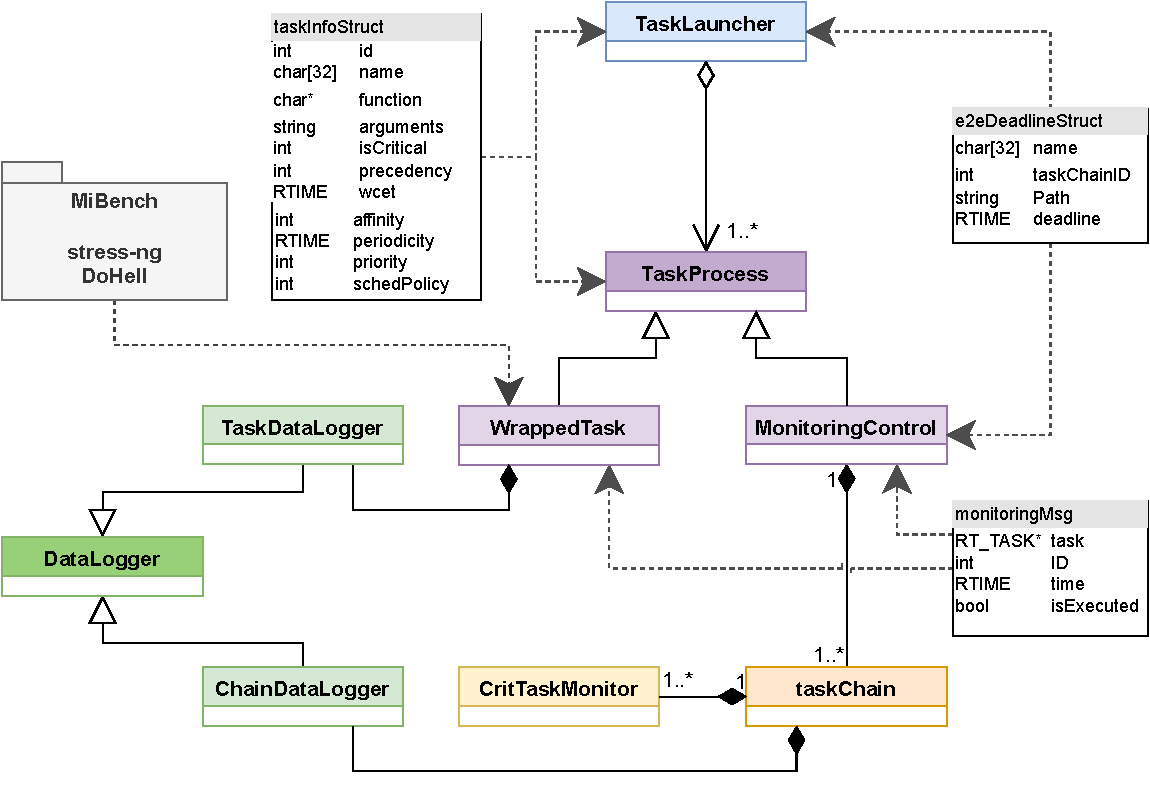
\includegraphics[width=\linewidth]{schemas/Implementation_DiagrammeDeClasse}
		\vspace{-25pt}
		\caption{Architecture Logicielle du Framework}
		\label{fig:implementationdiagrammedeclasse}
	\end{figure}
    
    Sur ce diagramme de classe simplifié figure en \textcolor{blue}{bleu} le module de mise en place et de lancement expérimental décrit précédemment, en \textcolor{violet}{violet} les classes qui permettent de lancer des tâches (que ce soit l'agent de contrôle ou les tâches à exécuter, critiques et non critiques), avec en \textcolor{orange}{orange} les structures mémoire de gestion de l'État de la chaîne de tâche et des tâches critiques, et pour finir en \textcolor{ForestGreen}{vert} les modules supplémentaires d'enregistrement des logs détaillés d'exécution pour être enregistrés, que ce soit pour la chaîne de tâche et pour les tâches individuelles. On retrouve aussi les structures de gestion des fichiers de configuration d'entrée, ainsi que la structure des messages asynchrones échangés entre les tâches critiques et l'Agent de Surveillance.
    
	Tous les éléments de la plateforme expérimentale ont ainsi été présentés, avec les choix que nous avons adoptés. Nous présentons dans la suite son exploitation par la mise en application du protocole expérimental global présenté au~\autoref{chap:4_ProtocolExpe}.
    	
\section{Application du Protocole Expérimental à MiBench}

	L'utilisation de MiBench de façon à être au plus proche d'un cas d'utilisation réel qui embarquerait des logiciels à criticité mixte présente à la fois des avantages et inconvénients. Il permet d'un côté d'exploiter directement un ensemble de tâches déjà reconnu et prêt à l'emploi, sur lequel les comportements ont été étudiés (utilisation de cache, charge CPU, entrées/sorties...). En revanche, il n'a pas été programmé initialement dans le but d'être exploité dans le cadre d'un système ne serait-ce que partiellement temps-réel. Par conséquent, la façon dont les tâches sont codées peut ne pas correspondre parfaitement à nos besoins, notamment via des incompatibilités entre les stratégies d'ordonnancement temps-réel et les appels de fonctions internes à ces programmes.
	Par conséquent, il est important d'appliquer le protocole d'implémentation de façon à caractériser correctement cet ensemble de tâches au sein de notre framework. Cela permet d'en exclure les éventuelles tâches qui ne sont pas adaptées. Comme nous l'avons mentionné au chapitre précédent, il y a particulièrement 3 raisons fondamentales qui vont justifier l'exclusion d'une tâche~: 
	\begin{itemize}
		\item de trop grands écarts en temps d'exécution comparé au reste des tâches \\
		(\textit{par exemple une tâche qui s'exécute pendant plusieurs centaines de millisecondes, contre la dizaine de millisecondes pour les autres}). De fait, il a été constaté dans le cadre des systèmes réels que dans une grande majorité des cas, les tâches temps-réel qui cohabitent sur un même processeurs ont des temps d'exécution qui sont du même ordre de grandeur. Cela vient du fait que si une tâche avait un temps d'exécution bien plus grand que les autres, elles semblerait presque paralyser l'exécution du reste des tâches le temps de sa terminaison. Il s'agit alors de tâches que l'on ne peut garder que pour des usages non-critiques à faible niveau de priorité.
		\item l'utilisation répétée de fonctions qui forcent des changements de domaine d'exécution entre Linux et Xenomai, cela provoque des délais supplémentaires variables et casse potentiellement l'ordonnancement,
		\item une trop forte irrégularité de comportement, \\
		(\textit{par exemple une tâche qui successivement dans les mêmes conditions apparentes peut avoir un temps d'exécution allant du simple au décuple}), 
	\end{itemize}
	De plus, même pour les tâches conservées ces données sont utiles, car elles donnent des pistes pour identifier si ces tâches ont plutôt un profil de tâche non-critique type "Best-Effort", ou bien de tâche critique temps-réel. 
	
\subsection{Phase de Conception}
Dans un premier temps, nous appliquons les étapes de caractérisation et conception présentées dans le protocole général illustré en~\autoref{tab:tableprotocoleComplet}. Elles correspondent à la caractérisation des tâches de façon individuelle, pour constituer le cas de test (chaîne de tâches critiques et tâches non critiques) et la caractérisation de la chaîne de tâches critiques.

\subsubsection{Profil des tâches individuelles (\ctxt{1} \& \ctxt{2})}
Tout d'abord pour la caractérisation des tâches MiBench listées en~\autoref{tab:MiBench_final}, elles sont exécutées individuellement (en isolation) pour une durée de test de 120 secondes, d'abord à une période de 100ms entre chaque job. Le test est effectué à nouveau mais accompagné de la charge de stress du calculateur tel que présenté précédemment. À l'issue de ces 2 mesures exécutées sur chacune des 23 tâches MiBench, chacune en version "Petite" et "Grande", cela donne $2*23*2 = 92$ expérimentations qui donnent les résultats détaillés de temps d'exécution ainsi que le nombre de changements de mode domaine et d'appels systèmes. Nous avons testé pour la charge de stress à la fois \texttt{stress-ng} et \texttt{doHell} et il s'avère que les résultats sont relativement similaires.
%de chacune des tâches en isolation et sous stress pour une durée de 120 secondes,

À l'issue de cela, on a pu classifier les tâches en 4 catégories, suivant leur sensibilité relative au stress (écart entre les temps d'exécution en isolation et sous stress), leur durée moyenne d'exécution, et le nombre de changements de modes~: 
\begin{itemize}
	\item CLEAN -- les tâches sont peu influencées par le stress, peu voire pas d'appels systèmes et changements de modes, temps d'exécution dans la moyenne.
	\item NOISE -- sensibilité au stress notable, temps d'exécution plutôt au-dessus de la moyenne avec du stress.
	\item OVERHEAD -- très forte sensibilité au stress, avec des appels systèmes en plus qui donnent des temps d'exécution très élevés en stress.
	\item REJECT -- Comportement erratique, avec de très fortes variations de temps d'exécution, ou bien temps d'exécution à un ordre de grandeur différent comparés à la moyenne.
\end{itemize}
Ce tri des tâches est résumé dans la~\autoref{tab:MiBench_classify}. Au vu des résultats, nous excluons les tâches REJECT qui ont un comportement trop éloigné de nos critères. Les tâches OVERHEAD pourraient servir de tâches non critiques, mais ce sera à employer avec précaution et de façon très limitée à cause des temps d'exécution élevés qui risquent de rendre le système non ordonnançable très facilement. Les tâches NOISE pourront servir de tâches non critiques et au sein de la chaîne de tâches critiques dans une certaine mesure pour y apporter la sensibilité au stress que l'on souhaite prévenir. Enfin, les tâches CLEAN semblent parfaitement correspondre en tant que tâches temps-réels qui représentent des blocs de code peu sensibles au stress. Cette classification peut tout autant servir pour mieux connaître et exploiter des tâches afin d'en constituer un cas de test "artificiel" comme nous le faisons ici, mais aussi dans un cas industriel pour définir les tâches les plus sensibles ou les plus provocatrices de stress par utilisation des ressources partagées. Cela pourrait permettre d'identifier les blocs logiciels problématiques sur lesquels il faudrait ajouter des mécanismes de controle supplémentaires, voire demander un nouveau développement pour atténuer voire corriger le problème.
 \smallbreak 
 
\begin{table}[ht]
	%\renewcommand{\arraystretch}{1.3} 	%% increase table row spacing, adjust to taste
	\caption{Tâches MiBench classifiées}
	\label{tab:MiBench_classify}
	\centering
	\begin{tabularx}{\textwidth}{lX} %%{@{}lX@{}}
		\toprule
		Domaine		& Tâches					\\
		\midrule
		CLEAN  		& fft-P, fft-G, fft-inv-P, basicmath-P, basicmath-G, bitcount-P						\\
		NOISE     	& jpeg-D-P, susan-corners-P, susan-smooth-P, susan-edges-P, sha-P, gsm-Toast-P, gsm-UToast-P, fft-inv-G, rijndael-E-P, adpcm-C-P, sha-G, susan-corners-G, susan-edges-G 		   					\\
		OVERHEAD    & stringsearch-G, jpeg-C-P, rijndael-D-P, jpeg-D-G, jpeg-C-G, adpcm-D-P, susan-smooth-G	   	\\
		REJECT      & rijndael-D-G, adpcm-D-G, gsm-Toast-G, adpcm-C-G, gsm-UToast-G, rijndael-E-G (\textit{trop longues}), \\
					& qsort-P, qsort-G, patricia-P, patricia-G, blowfish-E-P, blowfish-D-G, blowfish-D-P, blowfish-E-G (\textit{trop courtes})				\\
		\bottomrule
		\multicolumn{2}{c}{(\textit{-P/-G = version Petite/Grande ; -D/-E = Decode/enCode}) }
	\end{tabularx}
\end{table}

 Le détail des résultats de temps d’exécution obtenus lors de la caractérisation de chacune des tâches MiBench figure dans le~\autoref{tab:Phase1-2-results} en Annexe. Avec ces données, on a constaté que la majorité des temps d'exécution des tâches MiBench étaient de l'ordre de la dizaine de millisecondes, allant de 2-3ms pour les plus courtes à 30-40ms pour les plus longues. On a aussi pu constater un nombre de changements de domaine d'exécution "de base" de 58 changements, qui sont dûs à la phase de configuration de l'expérimentation et à la phase de terminaison avec l'écriture des logs. Ainsi, des tâches comme adpcm-C-G (version Grande, option enCodage) avec un temps d'exécution moyen de 432 ms sont rejetées. Notons qu'à l'inverse certaines tâches comme qsort ont été écartées parce qu'elles avaient un temps d'exécution bien trop court, de l'ordre de microsecondes. Cela n'étant pas normal, car ces tâches présentaient des temps d'exécution plus élevés quand utilisées en dehors de notre framework (version non modifiée). On suppose donc une incompatibilité avec notre framework de test qui n'a pas pu être levée.

\cmnt{
\begin{table}[ht!]
	\centering
	\caption{Tasks profiles in \textit{Xenomai} environment}
	\begin{tabular}{@{}lrrcrr@{}}
		\toprule
		Task & \multicolumn{2}{c}{execution times (ms)} & \phantom{} & \multicolumn{2}{c}{System Counters} \\ % pas sûr
		\cmidrule{2-3} \cmidrule{5-6}
		&   Median      &   Max    &&   Mode Switch & Sys. Call     \\
		\midrule
		Patricia    &   0.026       &   0.099       &&  10051        & 10338    \\
		FFT         &   7.36        &   7.39        &&  58           & 2343      \\
		rijndaelE   &   140,11      &   141.81      &&  158          & 446       \\
		\bottomrule
	\end{tabular}
	\label{tab:xenoIsol}
\end{table}
}

\cmnt{
	\begin{table}[ht]
	\centering
	\caption{Extrait profil des tâches}
	\label{tab:Stress}
	\begin{tabular}{@{}lrrcrr@{}}  %% r = right | l = left | c = center
		\toprule
		Tâche & \multicolumn{2}{c}{temps en isolation} & \phantom{}& \multicolumn{2}{c}{temps sous stress} \\
		\cmidrule{2-3} \cmidrule{5-6} 
					  &   Median (ms) &   Max (ms)  &&   Median (ms) &  Max (ms) \\
		\midrule
		djpeg-D-S     &   1.97		  &   2.28    	&&   19.91       &	211.53   \\
		rjindael-D-S  &   8.80    	  &   9.77   	&&   35.02       & 	526.33   \\
		FFT-S	      &   1.85    	  &   1.86    	&&    2.03       &	14.8     \\
		FFT$^{-1}$-S  &   3.56    	  &   3.57    	&&    4.05       &	19.74    \\
		bitcount-S    &   8.36    	  &   9.52    	&&    9.98       &	45.18    \\
		\bottomrule
	\end{tabular}
	\label{tab:xenoIsolMinMax}
\end{table}
}

\subsubsection{Profil de la Chaîne de tâches (\ctxt{3} \& \ctxt{4})}
À partir de la caractérisation des tâches, on spécifie la chaîne de tâches critiques, composée de 5 tâches~: \\
\centerline{ $ FFT \rightarrow Bitcount  \rightarrow Basicmath  \rightarrow FFT^{-1} \rightarrow sha $.}

Au regard des profils de temps d'exécution des tâches mesurés précédemment, le fichier d'entrée décrivant l'ensemble des paramètres de la chaîne est déclaré comme suit~: 
\begin{lstlisting}[caption={Chaine de tâche sélectionnée}, numbers=none, label={code:taskChain.in}]
ID pre name        FUNC     P   T rWCRT  A ARGS
 1   0 fft_S       fft     10  40    xx  2 8 2048 >[output]
 2   1 bitcount_S  bitcnts 10  60    xx  2 75000  >[output]
 4   2 bmath_S     math_s  10  40    xx  2 >[output]
 6   4 fft_inv_S   fft     10  40    xx  2 8 4096 -i >[output]
 7   6 sha_S       sha     10  60    xx  2 <[input]  >[output]
\end{lstlisting}

Bien entendu, avant la phase \ctxt{3} de caractérisation de la chaîne de tâches critiques en l'exécutant en isolation, la colonne des $rWCRT(\tau_i)$ est non renseignée.

La chaîne de tâches critiques est exécutée dans deux conditions différentes, en isolation à l'image du mode dégradé\footnote{\textbf{Mode Dégradé --} Pour rappel, le mode dégradé correspond, avec notre mécanisme, à l'arrêt temporaire des tâches non critiques pour exécuter les tâches critiques en isolation sur un cœur dédié.} (c.f. étape \ctxt{3}), et avec un stress imposé via stress-ng (c.f. étape \ctxt{4}). Cela permet d'une part de déterminer une échéance d'exécution bout-en-bout en adéquation avec le profil d'exécution de la chaîne, et de vérifier la pertinence de tester notre mécanisme en constatant une influence des interférences sur les temps de réponse bout-en-bout.
\smallbreak
\begin{table}[ht]
	\centering
	\caption{Profil de la chaîne de tâches critique - isolée et avec stress-ng}
	\label{tab:TaskChain_IsolStress}
	\begin{tabular}{@{}lrrrcrrr@{}}  %% r = right | l = left | c = center
		\toprule
		& \multicolumn{3}{c}{temps en isolation} &\phantom&\multicolumn{3}{c}{temps sous stress} \\
		\cmidrule{2-4} \cmidrule{6-8} 
		&   Min  & Moyen &  Max   &&  Min  & Moyen & Max 		\\
		\midrule
		temps de réponse (ms) &  90.11 & 125.85 & 130.06 && 90.18 & 164.00 & 306.87  	\\
		\bottomrule
	\end{tabular}
\end{table} 


Sur 120 secondes d'expérimentation, on obtient 1985 exécutions bout-en-bout de la chaîne de tâche en isolation, de même avec le stress imposé. On obtient alors un profil d'exécution, qui agrège tous les temps de réponses qui ont été mesurés. Le profil obtenu est représenté dans la~\autoref{graph:taskchainsansinterference}. Au regard de ces mesures, on identifie le temps d'exécution nominal de la chaîne de tâche qui est autour des 130\,ms et on peut alors définir une échéance de temps de réponse bout-en-bout arbitraire $D_C = 200\,ms$, près du double du temps de réponse bout-en-bout. Les détails des mesures de temps de réponse moyen et maximum en isolation et avec le stress forcé sont indiqués dans la~\autoref{tab:TaskChain_IsolStress}. On confirme la sensibilité de la chaîne à des interférences forcées, avec un pire cas à 300\,ms de temps de réponse bout-en-bout. De façon générale, on remarque un glissement du temps d'exécution moyen de 40\,ms supplémentaires, ce qui correspond à une période des tâches à la fréquence d’occurrence la plus forte.

\begin{figure}[ht]
	\centering
	\scalebox{0.9}{%% Creator: Matplotlib, PGF backend
%%
%% To include the figure in your LaTeX document, write
%%   \input{<filename>.pgf}
%%
%% Make sure the required packages are loaded in your preamble
%%   \usepackage{pgf}
%%
%% and, on pdftex
%%   \usepackage[utf8]{inputenc}\DeclareUnicodeCharacter{2212}{-}
%%
%% or, on luatex and xetex
%%   \usepackage{unicode-math}
%%
%% Figures using additional raster images can only be included by \input if
%% they are in the same directory as the main LaTeX file. For loading figures
%% from other directories you can use the `import` package
%%   \usepackage{import}
%%
%% and then include the figures with
%%   \import{<path to file>}{<filename>.pgf}
%%
%% Matplotlib used the following preamble
%%   \usepackage{fontspec}
%%   \setmainfont{DejaVuSerif.ttf}[Path=/usr/local/lib/python3.6/dist-packages/matplotlib/mpl-data/fonts/ttf/]
%%   \setsansfont{DejaVuSans.ttf}[Path=/usr/local/lib/python3.6/dist-packages/matplotlib/mpl-data/fonts/ttf/]
%%   \setmonofont{DejaVuSansMono.ttf}[Path=/usr/local/lib/python3.6/dist-packages/matplotlib/mpl-data/fonts/ttf/]
%%
\begingroup%
\makeatletter%
\begin{pgfpicture}%
\pgfpathrectangle{\pgfpointorigin}{\pgfqpoint{6.400000in}{4.800000in}}%
\pgfusepath{use as bounding box, clip}%
\begin{pgfscope}%
\pgfsetbuttcap%
\pgfsetmiterjoin%
\definecolor{currentfill}{rgb}{1.000000,1.000000,1.000000}%
\pgfsetfillcolor{currentfill}%
\pgfsetlinewidth{0.000000pt}%
\definecolor{currentstroke}{rgb}{1.000000,1.000000,1.000000}%
\pgfsetstrokecolor{currentstroke}%
\pgfsetdash{}{0pt}%
\pgfpathmoveto{\pgfqpoint{0.000000in}{0.000000in}}%
\pgfpathlineto{\pgfqpoint{6.400000in}{0.000000in}}%
\pgfpathlineto{\pgfqpoint{6.400000in}{4.800000in}}%
\pgfpathlineto{\pgfqpoint{0.000000in}{4.800000in}}%
\pgfpathclose%
\pgfusepath{fill}%
\end{pgfscope}%
\begin{pgfscope}%
\pgfsetbuttcap%
\pgfsetmiterjoin%
\definecolor{currentfill}{rgb}{1.000000,1.000000,1.000000}%
\pgfsetfillcolor{currentfill}%
\pgfsetlinewidth{0.000000pt}%
\definecolor{currentstroke}{rgb}{0.000000,0.000000,0.000000}%
\pgfsetstrokecolor{currentstroke}%
\pgfsetstrokeopacity{0.000000}%
\pgfsetdash{}{0pt}%
\pgfpathmoveto{\pgfqpoint{0.800000in}{0.528000in}}%
\pgfpathlineto{\pgfqpoint{5.760000in}{0.528000in}}%
\pgfpathlineto{\pgfqpoint{5.760000in}{4.224000in}}%
\pgfpathlineto{\pgfqpoint{0.800000in}{4.224000in}}%
\pgfpathclose%
\pgfusepath{fill}%
\end{pgfscope}%
\begin{pgfscope}%
\pgfpathrectangle{\pgfqpoint{0.800000in}{0.528000in}}{\pgfqpoint{4.960000in}{3.696000in}}%
\pgfusepath{clip}%
\pgfsetroundcap%
\pgfsetroundjoin%
\pgfsetlinewidth{1.003750pt}%
\definecolor{currentstroke}{rgb}{0.800000,0.800000,0.800000}%
\pgfsetstrokecolor{currentstroke}%
\pgfsetdash{}{0pt}%
\pgfpathmoveto{\pgfqpoint{0.982991in}{0.528000in}}%
\pgfpathlineto{\pgfqpoint{0.982991in}{4.224000in}}%
\pgfusepath{stroke}%
\end{pgfscope}%
\begin{pgfscope}%
\definecolor{textcolor}{rgb}{0.150000,0.150000,0.150000}%
\pgfsetstrokecolor{textcolor}%
\pgfsetfillcolor{textcolor}%
\pgftext[x=0.982991in,y=0.396056in,,top]{\color{textcolor}\sffamily\fontsize{11.000000}{13.200000}\selectfont 80}%
\end{pgfscope}%
\begin{pgfscope}%
\pgfpathrectangle{\pgfqpoint{0.800000in}{0.528000in}}{\pgfqpoint{4.960000in}{3.696000in}}%
\pgfusepath{clip}%
\pgfsetroundcap%
\pgfsetroundjoin%
\pgfsetlinewidth{1.003750pt}%
\definecolor{currentstroke}{rgb}{0.800000,0.800000,0.800000}%
\pgfsetstrokecolor{currentstroke}%
\pgfsetdash{}{0pt}%
\pgfpathmoveto{\pgfqpoint{1.564331in}{0.528000in}}%
\pgfpathlineto{\pgfqpoint{1.564331in}{4.224000in}}%
\pgfusepath{stroke}%
\end{pgfscope}%
\begin{pgfscope}%
\definecolor{textcolor}{rgb}{0.150000,0.150000,0.150000}%
\pgfsetstrokecolor{textcolor}%
\pgfsetfillcolor{textcolor}%
\pgftext[x=1.564331in,y=0.396056in,,top]{\color{textcolor}\sffamily\fontsize{11.000000}{13.200000}\selectfont 100}%
\end{pgfscope}%
\begin{pgfscope}%
\pgfpathrectangle{\pgfqpoint{0.800000in}{0.528000in}}{\pgfqpoint{4.960000in}{3.696000in}}%
\pgfusepath{clip}%
\pgfsetroundcap%
\pgfsetroundjoin%
\pgfsetlinewidth{1.003750pt}%
\definecolor{currentstroke}{rgb}{0.800000,0.800000,0.800000}%
\pgfsetstrokecolor{currentstroke}%
\pgfsetdash{}{0pt}%
\pgfpathmoveto{\pgfqpoint{2.145672in}{0.528000in}}%
\pgfpathlineto{\pgfqpoint{2.145672in}{4.224000in}}%
\pgfusepath{stroke}%
\end{pgfscope}%
\begin{pgfscope}%
\definecolor{textcolor}{rgb}{0.150000,0.150000,0.150000}%
\pgfsetstrokecolor{textcolor}%
\pgfsetfillcolor{textcolor}%
\pgftext[x=2.145672in,y=0.396056in,,top]{\color{textcolor}\sffamily\fontsize{11.000000}{13.200000}\selectfont 120}%
\end{pgfscope}%
\begin{pgfscope}%
\pgfpathrectangle{\pgfqpoint{0.800000in}{0.528000in}}{\pgfqpoint{4.960000in}{3.696000in}}%
\pgfusepath{clip}%
\pgfsetroundcap%
\pgfsetroundjoin%
\pgfsetlinewidth{1.003750pt}%
\definecolor{currentstroke}{rgb}{0.800000,0.800000,0.800000}%
\pgfsetstrokecolor{currentstroke}%
\pgfsetdash{}{0pt}%
\pgfpathmoveto{\pgfqpoint{2.727012in}{0.528000in}}%
\pgfpathlineto{\pgfqpoint{2.727012in}{4.224000in}}%
\pgfusepath{stroke}%
\end{pgfscope}%
\begin{pgfscope}%
\definecolor{textcolor}{rgb}{0.150000,0.150000,0.150000}%
\pgfsetstrokecolor{textcolor}%
\pgfsetfillcolor{textcolor}%
\pgftext[x=2.727012in,y=0.396056in,,top]{\color{textcolor}\sffamily\fontsize{11.000000}{13.200000}\selectfont 140}%
\end{pgfscope}%
\begin{pgfscope}%
\pgfpathrectangle{\pgfqpoint{0.800000in}{0.528000in}}{\pgfqpoint{4.960000in}{3.696000in}}%
\pgfusepath{clip}%
\pgfsetroundcap%
\pgfsetroundjoin%
\pgfsetlinewidth{1.003750pt}%
\definecolor{currentstroke}{rgb}{0.800000,0.800000,0.800000}%
\pgfsetstrokecolor{currentstroke}%
\pgfsetdash{}{0pt}%
\pgfpathmoveto{\pgfqpoint{3.308352in}{0.528000in}}%
\pgfpathlineto{\pgfqpoint{3.308352in}{4.224000in}}%
\pgfusepath{stroke}%
\end{pgfscope}%
\begin{pgfscope}%
\definecolor{textcolor}{rgb}{0.150000,0.150000,0.150000}%
\pgfsetstrokecolor{textcolor}%
\pgfsetfillcolor{textcolor}%
\pgftext[x=3.308352in,y=0.396056in,,top]{\color{textcolor}\sffamily\fontsize{11.000000}{13.200000}\selectfont 160}%
\end{pgfscope}%
\begin{pgfscope}%
\pgfpathrectangle{\pgfqpoint{0.800000in}{0.528000in}}{\pgfqpoint{4.960000in}{3.696000in}}%
\pgfusepath{clip}%
\pgfsetroundcap%
\pgfsetroundjoin%
\pgfsetlinewidth{1.003750pt}%
\definecolor{currentstroke}{rgb}{0.800000,0.800000,0.800000}%
\pgfsetstrokecolor{currentstroke}%
\pgfsetdash{}{0pt}%
\pgfpathmoveto{\pgfqpoint{3.889692in}{0.528000in}}%
\pgfpathlineto{\pgfqpoint{3.889692in}{4.224000in}}%
\pgfusepath{stroke}%
\end{pgfscope}%
\begin{pgfscope}%
\definecolor{textcolor}{rgb}{0.150000,0.150000,0.150000}%
\pgfsetstrokecolor{textcolor}%
\pgfsetfillcolor{textcolor}%
\pgftext[x=3.889692in,y=0.396056in,,top]{\color{textcolor}\sffamily\fontsize{11.000000}{13.200000}\selectfont 180}%
\end{pgfscope}%
\begin{pgfscope}%
\pgfpathrectangle{\pgfqpoint{0.800000in}{0.528000in}}{\pgfqpoint{4.960000in}{3.696000in}}%
\pgfusepath{clip}%
\pgfsetroundcap%
\pgfsetroundjoin%
\pgfsetlinewidth{1.003750pt}%
\definecolor{currentstroke}{rgb}{0.800000,0.800000,0.800000}%
\pgfsetstrokecolor{currentstroke}%
\pgfsetdash{}{0pt}%
\pgfpathmoveto{\pgfqpoint{4.471032in}{0.528000in}}%
\pgfpathlineto{\pgfqpoint{4.471032in}{4.224000in}}%
\pgfusepath{stroke}%
\end{pgfscope}%
\begin{pgfscope}%
\definecolor{textcolor}{rgb}{0.150000,0.150000,0.150000}%
\pgfsetstrokecolor{textcolor}%
\pgfsetfillcolor{textcolor}%
\pgftext[x=4.471032in,y=0.396056in,,top]{\color{textcolor}\sffamily\fontsize{11.000000}{13.200000}\selectfont 200}%
\end{pgfscope}%
\begin{pgfscope}%
\pgfpathrectangle{\pgfqpoint{0.800000in}{0.528000in}}{\pgfqpoint{4.960000in}{3.696000in}}%
\pgfusepath{clip}%
\pgfsetroundcap%
\pgfsetroundjoin%
\pgfsetlinewidth{1.003750pt}%
\definecolor{currentstroke}{rgb}{0.800000,0.800000,0.800000}%
\pgfsetstrokecolor{currentstroke}%
\pgfsetdash{}{0pt}%
\pgfpathmoveto{\pgfqpoint{5.052373in}{0.528000in}}%
\pgfpathlineto{\pgfqpoint{5.052373in}{4.224000in}}%
\pgfusepath{stroke}%
\end{pgfscope}%
\begin{pgfscope}%
\definecolor{textcolor}{rgb}{0.150000,0.150000,0.150000}%
\pgfsetstrokecolor{textcolor}%
\pgfsetfillcolor{textcolor}%
\pgftext[x=5.052373in,y=0.396056in,,top]{\color{textcolor}\sffamily\fontsize{11.000000}{13.200000}\selectfont 220}%
\end{pgfscope}%
\begin{pgfscope}%
\pgfpathrectangle{\pgfqpoint{0.800000in}{0.528000in}}{\pgfqpoint{4.960000in}{3.696000in}}%
\pgfusepath{clip}%
\pgfsetroundcap%
\pgfsetroundjoin%
\pgfsetlinewidth{1.003750pt}%
\definecolor{currentstroke}{rgb}{0.800000,0.800000,0.800000}%
\pgfsetstrokecolor{currentstroke}%
\pgfsetdash{}{0pt}%
\pgfpathmoveto{\pgfqpoint{5.633713in}{0.528000in}}%
\pgfpathlineto{\pgfqpoint{5.633713in}{4.224000in}}%
\pgfusepath{stroke}%
\end{pgfscope}%
\begin{pgfscope}%
\definecolor{textcolor}{rgb}{0.150000,0.150000,0.150000}%
\pgfsetstrokecolor{textcolor}%
\pgfsetfillcolor{textcolor}%
\pgftext[x=5.633713in,y=0.396056in,,top]{\color{textcolor}\sffamily\fontsize{11.000000}{13.200000}\selectfont 240}%
\end{pgfscope}%
\begin{pgfscope}%
\definecolor{textcolor}{rgb}{0.150000,0.150000,0.150000}%
\pgfsetstrokecolor{textcolor}%
\pgfsetfillcolor{textcolor}%
\pgftext[x=3.280000in,y=0.192646in,,top]{\color{textcolor}\sffamily\fontsize{12.000000}{14.400000}\selectfont Temps de réponse bout-en-bout (ms)}%
\end{pgfscope}%
\begin{pgfscope}%
\pgfpathrectangle{\pgfqpoint{0.800000in}{0.528000in}}{\pgfqpoint{4.960000in}{3.696000in}}%
\pgfusepath{clip}%
\pgfsetroundcap%
\pgfsetroundjoin%
\pgfsetlinewidth{1.003750pt}%
\definecolor{currentstroke}{rgb}{0.800000,0.800000,0.800000}%
\pgfsetstrokecolor{currentstroke}%
\pgfsetdash{}{0pt}%
\pgfpathmoveto{\pgfqpoint{0.800000in}{0.528000in}}%
\pgfpathlineto{\pgfqpoint{5.760000in}{0.528000in}}%
\pgfusepath{stroke}%
\end{pgfscope}%
\begin{pgfscope}%
\definecolor{textcolor}{rgb}{0.150000,0.150000,0.150000}%
\pgfsetstrokecolor{textcolor}%
\pgfsetfillcolor{textcolor}%
\pgftext[x=0.527886in, y=0.469962in, left, base]{\color{textcolor}\sffamily\fontsize{11.000000}{13.200000}\selectfont 0\%}%
\end{pgfscope}%
\begin{pgfscope}%
\pgfpathrectangle{\pgfqpoint{0.800000in}{0.528000in}}{\pgfqpoint{4.960000in}{3.696000in}}%
\pgfusepath{clip}%
\pgfsetroundcap%
\pgfsetroundjoin%
\pgfsetlinewidth{1.003750pt}%
\definecolor{currentstroke}{rgb}{0.800000,0.800000,0.800000}%
\pgfsetstrokecolor{currentstroke}%
\pgfsetdash{}{0pt}%
\pgfpathmoveto{\pgfqpoint{0.800000in}{1.274913in}}%
\pgfpathlineto{\pgfqpoint{5.760000in}{1.274913in}}%
\pgfusepath{stroke}%
\end{pgfscope}%
\begin{pgfscope}%
\definecolor{textcolor}{rgb}{0.150000,0.150000,0.150000}%
\pgfsetstrokecolor{textcolor}%
\pgfsetfillcolor{textcolor}%
\pgftext[x=0.527886in, y=1.216875in, left, base]{\color{textcolor}\sffamily\fontsize{11.000000}{13.200000}\selectfont 2\%}%
\end{pgfscope}%
\begin{pgfscope}%
\pgfpathrectangle{\pgfqpoint{0.800000in}{0.528000in}}{\pgfqpoint{4.960000in}{3.696000in}}%
\pgfusepath{clip}%
\pgfsetroundcap%
\pgfsetroundjoin%
\pgfsetlinewidth{1.003750pt}%
\definecolor{currentstroke}{rgb}{0.800000,0.800000,0.800000}%
\pgfsetstrokecolor{currentstroke}%
\pgfsetdash{}{0pt}%
\pgfpathmoveto{\pgfqpoint{0.800000in}{2.021825in}}%
\pgfpathlineto{\pgfqpoint{5.760000in}{2.021825in}}%
\pgfusepath{stroke}%
\end{pgfscope}%
\begin{pgfscope}%
\definecolor{textcolor}{rgb}{0.150000,0.150000,0.150000}%
\pgfsetstrokecolor{textcolor}%
\pgfsetfillcolor{textcolor}%
\pgftext[x=0.527886in, y=1.963788in, left, base]{\color{textcolor}\sffamily\fontsize{11.000000}{13.200000}\selectfont 4\%}%
\end{pgfscope}%
\begin{pgfscope}%
\pgfpathrectangle{\pgfqpoint{0.800000in}{0.528000in}}{\pgfqpoint{4.960000in}{3.696000in}}%
\pgfusepath{clip}%
\pgfsetroundcap%
\pgfsetroundjoin%
\pgfsetlinewidth{1.003750pt}%
\definecolor{currentstroke}{rgb}{0.800000,0.800000,0.800000}%
\pgfsetstrokecolor{currentstroke}%
\pgfsetdash{}{0pt}%
\pgfpathmoveto{\pgfqpoint{0.800000in}{2.768738in}}%
\pgfpathlineto{\pgfqpoint{5.760000in}{2.768738in}}%
\pgfusepath{stroke}%
\end{pgfscope}%
\begin{pgfscope}%
\definecolor{textcolor}{rgb}{0.150000,0.150000,0.150000}%
\pgfsetstrokecolor{textcolor}%
\pgfsetfillcolor{textcolor}%
\pgftext[x=0.527886in, y=2.710700in, left, base]{\color{textcolor}\sffamily\fontsize{11.000000}{13.200000}\selectfont 6\%}%
\end{pgfscope}%
\begin{pgfscope}%
\pgfpathrectangle{\pgfqpoint{0.800000in}{0.528000in}}{\pgfqpoint{4.960000in}{3.696000in}}%
\pgfusepath{clip}%
\pgfsetroundcap%
\pgfsetroundjoin%
\pgfsetlinewidth{1.003750pt}%
\definecolor{currentstroke}{rgb}{0.800000,0.800000,0.800000}%
\pgfsetstrokecolor{currentstroke}%
\pgfsetdash{}{0pt}%
\pgfpathmoveto{\pgfqpoint{0.800000in}{3.515650in}}%
\pgfpathlineto{\pgfqpoint{5.760000in}{3.515650in}}%
\pgfusepath{stroke}%
\end{pgfscope}%
\begin{pgfscope}%
\definecolor{textcolor}{rgb}{0.150000,0.150000,0.150000}%
\pgfsetstrokecolor{textcolor}%
\pgfsetfillcolor{textcolor}%
\pgftext[x=0.527886in, y=3.457613in, left, base]{\color{textcolor}\sffamily\fontsize{11.000000}{13.200000}\selectfont 8\%}%
\end{pgfscope}%
\begin{pgfscope}%
\definecolor{textcolor}{rgb}{0.150000,0.150000,0.150000}%
\pgfsetstrokecolor{textcolor}%
\pgfsetfillcolor{textcolor}%
\pgftext[x=0.272331in,y=2.376000in,,bottom,rotate=90.000000]{\color{textcolor}\sffamily\fontsize{12.000000}{14.400000}\selectfont Densité de distribution}%
\end{pgfscope}%
\begin{pgfscope}%
\pgfpathrectangle{\pgfqpoint{0.800000in}{0.528000in}}{\pgfqpoint{4.960000in}{3.696000in}}%
\pgfusepath{clip}%
\pgfsetbuttcap%
\pgfsetroundjoin%
\definecolor{currentfill}{rgb}{0.018039,0.067059,0.550196}%
\pgfsetfillcolor{currentfill}%
\pgfsetfillopacity{0.250000}%
\pgfsetlinewidth{1.003750pt}%
\definecolor{currentstroke}{rgb}{0.018039,0.067059,0.550196}%
\pgfsetstrokecolor{currentstroke}%
\pgfsetdash{}{0pt}%
\pgfsys@defobject{currentmarker}{\pgfqpoint{1.025455in}{0.528000in}}{\pgfqpoint{2.674537in}{2.186749in}}{%
\pgfpathmoveto{\pgfqpoint{1.025455in}{0.529344in}}%
\pgfpathlineto{\pgfqpoint{1.025455in}{0.528000in}}%
\pgfpathlineto{\pgfqpoint{1.033741in}{0.528000in}}%
\pgfpathlineto{\pgfqpoint{1.042028in}{0.528000in}}%
\pgfpathlineto{\pgfqpoint{1.050315in}{0.528000in}}%
\pgfpathlineto{\pgfqpoint{1.058602in}{0.528000in}}%
\pgfpathlineto{\pgfqpoint{1.066889in}{0.528000in}}%
\pgfpathlineto{\pgfqpoint{1.075176in}{0.528000in}}%
\pgfpathlineto{\pgfqpoint{1.083462in}{0.528000in}}%
\pgfpathlineto{\pgfqpoint{1.091749in}{0.528000in}}%
\pgfpathlineto{\pgfqpoint{1.100036in}{0.528000in}}%
\pgfpathlineto{\pgfqpoint{1.108323in}{0.528000in}}%
\pgfpathlineto{\pgfqpoint{1.116610in}{0.528000in}}%
\pgfpathlineto{\pgfqpoint{1.124897in}{0.528000in}}%
\pgfpathlineto{\pgfqpoint{1.133184in}{0.528000in}}%
\pgfpathlineto{\pgfqpoint{1.141470in}{0.528000in}}%
\pgfpathlineto{\pgfqpoint{1.149757in}{0.528000in}}%
\pgfpathlineto{\pgfqpoint{1.158044in}{0.528000in}}%
\pgfpathlineto{\pgfqpoint{1.166331in}{0.528000in}}%
\pgfpathlineto{\pgfqpoint{1.174618in}{0.528000in}}%
\pgfpathlineto{\pgfqpoint{1.182905in}{0.528000in}}%
\pgfpathlineto{\pgfqpoint{1.191191in}{0.528000in}}%
\pgfpathlineto{\pgfqpoint{1.199478in}{0.528000in}}%
\pgfpathlineto{\pgfqpoint{1.207765in}{0.528000in}}%
\pgfpathlineto{\pgfqpoint{1.216052in}{0.528000in}}%
\pgfpathlineto{\pgfqpoint{1.224339in}{0.528000in}}%
\pgfpathlineto{\pgfqpoint{1.232626in}{0.528000in}}%
\pgfpathlineto{\pgfqpoint{1.240913in}{0.528000in}}%
\pgfpathlineto{\pgfqpoint{1.249199in}{0.528000in}}%
\pgfpathlineto{\pgfqpoint{1.257486in}{0.528000in}}%
\pgfpathlineto{\pgfqpoint{1.265773in}{0.528000in}}%
\pgfpathlineto{\pgfqpoint{1.274060in}{0.528000in}}%
\pgfpathlineto{\pgfqpoint{1.282347in}{0.528000in}}%
\pgfpathlineto{\pgfqpoint{1.290634in}{0.528000in}}%
\pgfpathlineto{\pgfqpoint{1.298920in}{0.528000in}}%
\pgfpathlineto{\pgfqpoint{1.307207in}{0.528000in}}%
\pgfpathlineto{\pgfqpoint{1.315494in}{0.528000in}}%
\pgfpathlineto{\pgfqpoint{1.323781in}{0.528000in}}%
\pgfpathlineto{\pgfqpoint{1.332068in}{0.528000in}}%
\pgfpathlineto{\pgfqpoint{1.340355in}{0.528000in}}%
\pgfpathlineto{\pgfqpoint{1.348642in}{0.528000in}}%
\pgfpathlineto{\pgfqpoint{1.356928in}{0.528000in}}%
\pgfpathlineto{\pgfqpoint{1.365215in}{0.528000in}}%
\pgfpathlineto{\pgfqpoint{1.373502in}{0.528000in}}%
\pgfpathlineto{\pgfqpoint{1.381789in}{0.528000in}}%
\pgfpathlineto{\pgfqpoint{1.390076in}{0.528000in}}%
\pgfpathlineto{\pgfqpoint{1.398363in}{0.528000in}}%
\pgfpathlineto{\pgfqpoint{1.406650in}{0.528000in}}%
\pgfpathlineto{\pgfqpoint{1.414936in}{0.528000in}}%
\pgfpathlineto{\pgfqpoint{1.423223in}{0.528000in}}%
\pgfpathlineto{\pgfqpoint{1.431510in}{0.528000in}}%
\pgfpathlineto{\pgfqpoint{1.439797in}{0.528000in}}%
\pgfpathlineto{\pgfqpoint{1.448084in}{0.528000in}}%
\pgfpathlineto{\pgfqpoint{1.456371in}{0.528000in}}%
\pgfpathlineto{\pgfqpoint{1.464657in}{0.528000in}}%
\pgfpathlineto{\pgfqpoint{1.472944in}{0.528000in}}%
\pgfpathlineto{\pgfqpoint{1.481231in}{0.528000in}}%
\pgfpathlineto{\pgfqpoint{1.489518in}{0.528000in}}%
\pgfpathlineto{\pgfqpoint{1.497805in}{0.528000in}}%
\pgfpathlineto{\pgfqpoint{1.506092in}{0.528000in}}%
\pgfpathlineto{\pgfqpoint{1.514379in}{0.528000in}}%
\pgfpathlineto{\pgfqpoint{1.522665in}{0.528000in}}%
\pgfpathlineto{\pgfqpoint{1.530952in}{0.528000in}}%
\pgfpathlineto{\pgfqpoint{1.539239in}{0.528000in}}%
\pgfpathlineto{\pgfqpoint{1.547526in}{0.528000in}}%
\pgfpathlineto{\pgfqpoint{1.555813in}{0.528000in}}%
\pgfpathlineto{\pgfqpoint{1.564100in}{0.528000in}}%
\pgfpathlineto{\pgfqpoint{1.572386in}{0.528000in}}%
\pgfpathlineto{\pgfqpoint{1.580673in}{0.528000in}}%
\pgfpathlineto{\pgfqpoint{1.588960in}{0.528000in}}%
\pgfpathlineto{\pgfqpoint{1.597247in}{0.528000in}}%
\pgfpathlineto{\pgfqpoint{1.605534in}{0.528000in}}%
\pgfpathlineto{\pgfqpoint{1.613821in}{0.528000in}}%
\pgfpathlineto{\pgfqpoint{1.622108in}{0.528000in}}%
\pgfpathlineto{\pgfqpoint{1.630394in}{0.528000in}}%
\pgfpathlineto{\pgfqpoint{1.638681in}{0.528000in}}%
\pgfpathlineto{\pgfqpoint{1.646968in}{0.528000in}}%
\pgfpathlineto{\pgfqpoint{1.655255in}{0.528000in}}%
\pgfpathlineto{\pgfqpoint{1.663542in}{0.528000in}}%
\pgfpathlineto{\pgfqpoint{1.671829in}{0.528000in}}%
\pgfpathlineto{\pgfqpoint{1.680115in}{0.528000in}}%
\pgfpathlineto{\pgfqpoint{1.688402in}{0.528000in}}%
\pgfpathlineto{\pgfqpoint{1.696689in}{0.528000in}}%
\pgfpathlineto{\pgfqpoint{1.704976in}{0.528000in}}%
\pgfpathlineto{\pgfqpoint{1.713263in}{0.528000in}}%
\pgfpathlineto{\pgfqpoint{1.721550in}{0.528000in}}%
\pgfpathlineto{\pgfqpoint{1.729837in}{0.528000in}}%
\pgfpathlineto{\pgfqpoint{1.738123in}{0.528000in}}%
\pgfpathlineto{\pgfqpoint{1.746410in}{0.528000in}}%
\pgfpathlineto{\pgfqpoint{1.754697in}{0.528000in}}%
\pgfpathlineto{\pgfqpoint{1.762984in}{0.528000in}}%
\pgfpathlineto{\pgfqpoint{1.771271in}{0.528000in}}%
\pgfpathlineto{\pgfqpoint{1.779558in}{0.528000in}}%
\pgfpathlineto{\pgfqpoint{1.787844in}{0.528000in}}%
\pgfpathlineto{\pgfqpoint{1.796131in}{0.528000in}}%
\pgfpathlineto{\pgfqpoint{1.804418in}{0.528000in}}%
\pgfpathlineto{\pgfqpoint{1.812705in}{0.528000in}}%
\pgfpathlineto{\pgfqpoint{1.820992in}{0.528000in}}%
\pgfpathlineto{\pgfqpoint{1.829279in}{0.528000in}}%
\pgfpathlineto{\pgfqpoint{1.837566in}{0.528000in}}%
\pgfpathlineto{\pgfqpoint{1.845852in}{0.528000in}}%
\pgfpathlineto{\pgfqpoint{1.854139in}{0.528000in}}%
\pgfpathlineto{\pgfqpoint{1.862426in}{0.528000in}}%
\pgfpathlineto{\pgfqpoint{1.870713in}{0.528000in}}%
\pgfpathlineto{\pgfqpoint{1.879000in}{0.528000in}}%
\pgfpathlineto{\pgfqpoint{1.887287in}{0.528000in}}%
\pgfpathlineto{\pgfqpoint{1.895573in}{0.528000in}}%
\pgfpathlineto{\pgfqpoint{1.903860in}{0.528000in}}%
\pgfpathlineto{\pgfqpoint{1.912147in}{0.528000in}}%
\pgfpathlineto{\pgfqpoint{1.920434in}{0.528000in}}%
\pgfpathlineto{\pgfqpoint{1.928721in}{0.528000in}}%
\pgfpathlineto{\pgfqpoint{1.937008in}{0.528000in}}%
\pgfpathlineto{\pgfqpoint{1.945295in}{0.528000in}}%
\pgfpathlineto{\pgfqpoint{1.953581in}{0.528000in}}%
\pgfpathlineto{\pgfqpoint{1.961868in}{0.528000in}}%
\pgfpathlineto{\pgfqpoint{1.970155in}{0.528000in}}%
\pgfpathlineto{\pgfqpoint{1.978442in}{0.528000in}}%
\pgfpathlineto{\pgfqpoint{1.986729in}{0.528000in}}%
\pgfpathlineto{\pgfqpoint{1.995016in}{0.528000in}}%
\pgfpathlineto{\pgfqpoint{2.003302in}{0.528000in}}%
\pgfpathlineto{\pgfqpoint{2.011589in}{0.528000in}}%
\pgfpathlineto{\pgfqpoint{2.019876in}{0.528000in}}%
\pgfpathlineto{\pgfqpoint{2.028163in}{0.528000in}}%
\pgfpathlineto{\pgfqpoint{2.036450in}{0.528000in}}%
\pgfpathlineto{\pgfqpoint{2.044737in}{0.528000in}}%
\pgfpathlineto{\pgfqpoint{2.053024in}{0.528000in}}%
\pgfpathlineto{\pgfqpoint{2.061310in}{0.528000in}}%
\pgfpathlineto{\pgfqpoint{2.069597in}{0.528000in}}%
\pgfpathlineto{\pgfqpoint{2.077884in}{0.528000in}}%
\pgfpathlineto{\pgfqpoint{2.086171in}{0.528000in}}%
\pgfpathlineto{\pgfqpoint{2.094458in}{0.528000in}}%
\pgfpathlineto{\pgfqpoint{2.102745in}{0.528000in}}%
\pgfpathlineto{\pgfqpoint{2.111032in}{0.528000in}}%
\pgfpathlineto{\pgfqpoint{2.119318in}{0.528000in}}%
\pgfpathlineto{\pgfqpoint{2.127605in}{0.528000in}}%
\pgfpathlineto{\pgfqpoint{2.135892in}{0.528000in}}%
\pgfpathlineto{\pgfqpoint{2.144179in}{0.528000in}}%
\pgfpathlineto{\pgfqpoint{2.152466in}{0.528000in}}%
\pgfpathlineto{\pgfqpoint{2.160753in}{0.528000in}}%
\pgfpathlineto{\pgfqpoint{2.169039in}{0.528000in}}%
\pgfpathlineto{\pgfqpoint{2.177326in}{0.528000in}}%
\pgfpathlineto{\pgfqpoint{2.185613in}{0.528000in}}%
\pgfpathlineto{\pgfqpoint{2.193900in}{0.528000in}}%
\pgfpathlineto{\pgfqpoint{2.202187in}{0.528000in}}%
\pgfpathlineto{\pgfqpoint{2.210474in}{0.528000in}}%
\pgfpathlineto{\pgfqpoint{2.218761in}{0.528000in}}%
\pgfpathlineto{\pgfqpoint{2.227047in}{0.528000in}}%
\pgfpathlineto{\pgfqpoint{2.235334in}{0.528000in}}%
\pgfpathlineto{\pgfqpoint{2.243621in}{0.528000in}}%
\pgfpathlineto{\pgfqpoint{2.251908in}{0.528000in}}%
\pgfpathlineto{\pgfqpoint{2.260195in}{0.528000in}}%
\pgfpathlineto{\pgfqpoint{2.268482in}{0.528000in}}%
\pgfpathlineto{\pgfqpoint{2.276768in}{0.528000in}}%
\pgfpathlineto{\pgfqpoint{2.285055in}{0.528000in}}%
\pgfpathlineto{\pgfqpoint{2.293342in}{0.528000in}}%
\pgfpathlineto{\pgfqpoint{2.301629in}{0.528000in}}%
\pgfpathlineto{\pgfqpoint{2.309916in}{0.528000in}}%
\pgfpathlineto{\pgfqpoint{2.318203in}{0.528000in}}%
\pgfpathlineto{\pgfqpoint{2.326490in}{0.528000in}}%
\pgfpathlineto{\pgfqpoint{2.334776in}{0.528000in}}%
\pgfpathlineto{\pgfqpoint{2.343063in}{0.528000in}}%
\pgfpathlineto{\pgfqpoint{2.351350in}{0.528000in}}%
\pgfpathlineto{\pgfqpoint{2.359637in}{0.528000in}}%
\pgfpathlineto{\pgfqpoint{2.367924in}{0.528000in}}%
\pgfpathlineto{\pgfqpoint{2.376211in}{0.528000in}}%
\pgfpathlineto{\pgfqpoint{2.384497in}{0.528000in}}%
\pgfpathlineto{\pgfqpoint{2.392784in}{0.528000in}}%
\pgfpathlineto{\pgfqpoint{2.401071in}{0.528000in}}%
\pgfpathlineto{\pgfqpoint{2.409358in}{0.528000in}}%
\pgfpathlineto{\pgfqpoint{2.417645in}{0.528000in}}%
\pgfpathlineto{\pgfqpoint{2.425932in}{0.528000in}}%
\pgfpathlineto{\pgfqpoint{2.434219in}{0.528000in}}%
\pgfpathlineto{\pgfqpoint{2.442505in}{0.528000in}}%
\pgfpathlineto{\pgfqpoint{2.450792in}{0.528000in}}%
\pgfpathlineto{\pgfqpoint{2.459079in}{0.528000in}}%
\pgfpathlineto{\pgfqpoint{2.467366in}{0.528000in}}%
\pgfpathlineto{\pgfqpoint{2.475653in}{0.528000in}}%
\pgfpathlineto{\pgfqpoint{2.483940in}{0.528000in}}%
\pgfpathlineto{\pgfqpoint{2.492226in}{0.528000in}}%
\pgfpathlineto{\pgfqpoint{2.500513in}{0.528000in}}%
\pgfpathlineto{\pgfqpoint{2.508800in}{0.528000in}}%
\pgfpathlineto{\pgfqpoint{2.517087in}{0.528000in}}%
\pgfpathlineto{\pgfqpoint{2.525374in}{0.528000in}}%
\pgfpathlineto{\pgfqpoint{2.533661in}{0.528000in}}%
\pgfpathlineto{\pgfqpoint{2.541948in}{0.528000in}}%
\pgfpathlineto{\pgfqpoint{2.550234in}{0.528000in}}%
\pgfpathlineto{\pgfqpoint{2.558521in}{0.528000in}}%
\pgfpathlineto{\pgfqpoint{2.566808in}{0.528000in}}%
\pgfpathlineto{\pgfqpoint{2.575095in}{0.528000in}}%
\pgfpathlineto{\pgfqpoint{2.583382in}{0.528000in}}%
\pgfpathlineto{\pgfqpoint{2.591669in}{0.528000in}}%
\pgfpathlineto{\pgfqpoint{2.599955in}{0.528000in}}%
\pgfpathlineto{\pgfqpoint{2.608242in}{0.528000in}}%
\pgfpathlineto{\pgfqpoint{2.616529in}{0.528000in}}%
\pgfpathlineto{\pgfqpoint{2.624816in}{0.528000in}}%
\pgfpathlineto{\pgfqpoint{2.633103in}{0.528000in}}%
\pgfpathlineto{\pgfqpoint{2.641390in}{0.528000in}}%
\pgfpathlineto{\pgfqpoint{2.649677in}{0.528000in}}%
\pgfpathlineto{\pgfqpoint{2.657963in}{0.528000in}}%
\pgfpathlineto{\pgfqpoint{2.666250in}{0.528000in}}%
\pgfpathlineto{\pgfqpoint{2.674537in}{0.528000in}}%
\pgfpathlineto{\pgfqpoint{2.674537in}{0.542142in}}%
\pgfpathlineto{\pgfqpoint{2.674537in}{0.542142in}}%
\pgfpathlineto{\pgfqpoint{2.666250in}{0.546986in}}%
\pgfpathlineto{\pgfqpoint{2.657963in}{0.553248in}}%
\pgfpathlineto{\pgfqpoint{2.649677in}{0.561258in}}%
\pgfpathlineto{\pgfqpoint{2.641390in}{0.571396in}}%
\pgfpathlineto{\pgfqpoint{2.633103in}{0.584088in}}%
\pgfpathlineto{\pgfqpoint{2.624816in}{0.599809in}}%
\pgfpathlineto{\pgfqpoint{2.616529in}{0.619069in}}%
\pgfpathlineto{\pgfqpoint{2.608242in}{0.642407in}}%
\pgfpathlineto{\pgfqpoint{2.599955in}{0.670372in}}%
\pgfpathlineto{\pgfqpoint{2.591669in}{0.703507in}}%
\pgfpathlineto{\pgfqpoint{2.583382in}{0.742320in}}%
\pgfpathlineto{\pgfqpoint{2.575095in}{0.787261in}}%
\pgfpathlineto{\pgfqpoint{2.566808in}{0.838687in}}%
\pgfpathlineto{\pgfqpoint{2.558521in}{0.896830in}}%
\pgfpathlineto{\pgfqpoint{2.550234in}{0.961761in}}%
\pgfpathlineto{\pgfqpoint{2.541948in}{1.033365in}}%
\pgfpathlineto{\pgfqpoint{2.533661in}{1.111306in}}%
\pgfpathlineto{\pgfqpoint{2.525374in}{1.195010in}}%
\pgfpathlineto{\pgfqpoint{2.517087in}{1.283650in}}%
\pgfpathlineto{\pgfqpoint{2.508800in}{1.376149in}}%
\pgfpathlineto{\pgfqpoint{2.500513in}{1.471181in}}%
\pgfpathlineto{\pgfqpoint{2.492226in}{1.567204in}}%
\pgfpathlineto{\pgfqpoint{2.483940in}{1.662490in}}%
\pgfpathlineto{\pgfqpoint{2.475653in}{1.755177in}}%
\pgfpathlineto{\pgfqpoint{2.467366in}{1.843325in}}%
\pgfpathlineto{\pgfqpoint{2.459079in}{1.924989in}}%
\pgfpathlineto{\pgfqpoint{2.450792in}{1.998285in}}%
\pgfpathlineto{\pgfqpoint{2.442505in}{2.061470in}}%
\pgfpathlineto{\pgfqpoint{2.434219in}{2.113007in}}%
\pgfpathlineto{\pgfqpoint{2.425932in}{2.151632in}}%
\pgfpathlineto{\pgfqpoint{2.417645in}{2.176405in}}%
\pgfpathlineto{\pgfqpoint{2.409358in}{2.186749in}}%
\pgfpathlineto{\pgfqpoint{2.401071in}{2.182472in}}%
\pgfpathlineto{\pgfqpoint{2.392784in}{2.163773in}}%
\pgfpathlineto{\pgfqpoint{2.384497in}{2.131229in}}%
\pgfpathlineto{\pgfqpoint{2.376211in}{2.085764in}}%
\pgfpathlineto{\pgfqpoint{2.367924in}{2.028608in}}%
\pgfpathlineto{\pgfqpoint{2.359637in}{1.961242in}}%
\pgfpathlineto{\pgfqpoint{2.351350in}{1.885331in}}%
\pgfpathlineto{\pgfqpoint{2.343063in}{1.802662in}}%
\pgfpathlineto{\pgfqpoint{2.334776in}{1.715068in}}%
\pgfpathlineto{\pgfqpoint{2.326490in}{1.624371in}}%
\pgfpathlineto{\pgfqpoint{2.318203in}{1.532315in}}%
\pgfpathlineto{\pgfqpoint{2.309916in}{1.440520in}}%
\pgfpathlineto{\pgfqpoint{2.301629in}{1.350441in}}%
\pgfpathlineto{\pgfqpoint{2.293342in}{1.263335in}}%
\pgfpathlineto{\pgfqpoint{2.285055in}{1.180247in}}%
\pgfpathlineto{\pgfqpoint{2.276768in}{1.102000in}}%
\pgfpathlineto{\pgfqpoint{2.268482in}{1.029199in}}%
\pgfpathlineto{\pgfqpoint{2.260195in}{0.962241in}}%
\pgfpathlineto{\pgfqpoint{2.251908in}{0.901332in}}%
\pgfpathlineto{\pgfqpoint{2.243621in}{0.846511in}}%
\pgfpathlineto{\pgfqpoint{2.235334in}{0.797670in}}%
\pgfpathlineto{\pgfqpoint{2.227047in}{0.754587in}}%
\pgfpathlineto{\pgfqpoint{2.218761in}{0.716948in}}%
\pgfpathlineto{\pgfqpoint{2.210474in}{0.684373in}}%
\pgfpathlineto{\pgfqpoint{2.202187in}{0.656440in}}%
\pgfpathlineto{\pgfqpoint{2.193900in}{0.632703in}}%
\pgfpathlineto{\pgfqpoint{2.185613in}{0.612709in}}%
\pgfpathlineto{\pgfqpoint{2.177326in}{0.596017in}}%
\pgfpathlineto{\pgfqpoint{2.169039in}{0.582201in}}%
\pgfpathlineto{\pgfqpoint{2.160753in}{0.570863in}}%
\pgfpathlineto{\pgfqpoint{2.152466in}{0.561638in}}%
\pgfpathlineto{\pgfqpoint{2.144179in}{0.554197in}}%
\pgfpathlineto{\pgfqpoint{2.135892in}{0.548244in}}%
\pgfpathlineto{\pgfqpoint{2.127605in}{0.543522in}}%
\pgfpathlineto{\pgfqpoint{2.119318in}{0.539809in}}%
\pgfpathlineto{\pgfqpoint{2.111032in}{0.536913in}}%
\pgfpathlineto{\pgfqpoint{2.102745in}{0.534674in}}%
\pgfpathlineto{\pgfqpoint{2.094458in}{0.532958in}}%
\pgfpathlineto{\pgfqpoint{2.086171in}{0.531653in}}%
\pgfpathlineto{\pgfqpoint{2.077884in}{0.530670in}}%
\pgfpathlineto{\pgfqpoint{2.069597in}{0.529935in}}%
\pgfpathlineto{\pgfqpoint{2.061310in}{0.529391in}}%
\pgfpathlineto{\pgfqpoint{2.053024in}{0.528992in}}%
\pgfpathlineto{\pgfqpoint{2.044737in}{0.528701in}}%
\pgfpathlineto{\pgfqpoint{2.036450in}{0.528491in}}%
\pgfpathlineto{\pgfqpoint{2.028163in}{0.528341in}}%
\pgfpathlineto{\pgfqpoint{2.019876in}{0.528235in}}%
\pgfpathlineto{\pgfqpoint{2.011589in}{0.528161in}}%
\pgfpathlineto{\pgfqpoint{2.003302in}{0.528109in}}%
\pgfpathlineto{\pgfqpoint{1.995016in}{0.528073in}}%
\pgfpathlineto{\pgfqpoint{1.986729in}{0.528049in}}%
\pgfpathlineto{\pgfqpoint{1.978442in}{0.528032in}}%
\pgfpathlineto{\pgfqpoint{1.970155in}{0.528021in}}%
\pgfpathlineto{\pgfqpoint{1.961868in}{0.528014in}}%
\pgfpathlineto{\pgfqpoint{1.953581in}{0.528009in}}%
\pgfpathlineto{\pgfqpoint{1.945295in}{0.528006in}}%
\pgfpathlineto{\pgfqpoint{1.937008in}{0.528004in}}%
\pgfpathlineto{\pgfqpoint{1.928721in}{0.528002in}}%
\pgfpathlineto{\pgfqpoint{1.920434in}{0.528001in}}%
\pgfpathlineto{\pgfqpoint{1.912147in}{0.528001in}}%
\pgfpathlineto{\pgfqpoint{1.903860in}{0.528001in}}%
\pgfpathlineto{\pgfqpoint{1.895573in}{0.528001in}}%
\pgfpathlineto{\pgfqpoint{1.887287in}{0.528001in}}%
\pgfpathlineto{\pgfqpoint{1.879000in}{0.528001in}}%
\pgfpathlineto{\pgfqpoint{1.870713in}{0.528001in}}%
\pgfpathlineto{\pgfqpoint{1.862426in}{0.528001in}}%
\pgfpathlineto{\pgfqpoint{1.854139in}{0.528002in}}%
\pgfpathlineto{\pgfqpoint{1.845852in}{0.528002in}}%
\pgfpathlineto{\pgfqpoint{1.837566in}{0.528003in}}%
\pgfpathlineto{\pgfqpoint{1.829279in}{0.528005in}}%
\pgfpathlineto{\pgfqpoint{1.820992in}{0.528007in}}%
\pgfpathlineto{\pgfqpoint{1.812705in}{0.528010in}}%
\pgfpathlineto{\pgfqpoint{1.804418in}{0.528014in}}%
\pgfpathlineto{\pgfqpoint{1.796131in}{0.528019in}}%
\pgfpathlineto{\pgfqpoint{1.787844in}{0.528026in}}%
\pgfpathlineto{\pgfqpoint{1.779558in}{0.528035in}}%
\pgfpathlineto{\pgfqpoint{1.771271in}{0.528048in}}%
\pgfpathlineto{\pgfqpoint{1.762984in}{0.528063in}}%
\pgfpathlineto{\pgfqpoint{1.754697in}{0.528084in}}%
\pgfpathlineto{\pgfqpoint{1.746410in}{0.528110in}}%
\pgfpathlineto{\pgfqpoint{1.738123in}{0.528142in}}%
\pgfpathlineto{\pgfqpoint{1.729837in}{0.528182in}}%
\pgfpathlineto{\pgfqpoint{1.721550in}{0.528232in}}%
\pgfpathlineto{\pgfqpoint{1.713263in}{0.528293in}}%
\pgfpathlineto{\pgfqpoint{1.704976in}{0.528366in}}%
\pgfpathlineto{\pgfqpoint{1.696689in}{0.528453in}}%
\pgfpathlineto{\pgfqpoint{1.688402in}{0.528557in}}%
\pgfpathlineto{\pgfqpoint{1.680115in}{0.528678in}}%
\pgfpathlineto{\pgfqpoint{1.671829in}{0.528820in}}%
\pgfpathlineto{\pgfqpoint{1.663542in}{0.528982in}}%
\pgfpathlineto{\pgfqpoint{1.655255in}{0.529168in}}%
\pgfpathlineto{\pgfqpoint{1.646968in}{0.529379in}}%
\pgfpathlineto{\pgfqpoint{1.638681in}{0.529616in}}%
\pgfpathlineto{\pgfqpoint{1.630394in}{0.529880in}}%
\pgfpathlineto{\pgfqpoint{1.622108in}{0.530175in}}%
\pgfpathlineto{\pgfqpoint{1.613821in}{0.530500in}}%
\pgfpathlineto{\pgfqpoint{1.605534in}{0.530858in}}%
\pgfpathlineto{\pgfqpoint{1.597247in}{0.531252in}}%
\pgfpathlineto{\pgfqpoint{1.588960in}{0.531685in}}%
\pgfpathlineto{\pgfqpoint{1.580673in}{0.532162in}}%
\pgfpathlineto{\pgfqpoint{1.572386in}{0.532687in}}%
\pgfpathlineto{\pgfqpoint{1.564100in}{0.533269in}}%
\pgfpathlineto{\pgfqpoint{1.555813in}{0.533916in}}%
\pgfpathlineto{\pgfqpoint{1.547526in}{0.534641in}}%
\pgfpathlineto{\pgfqpoint{1.539239in}{0.535458in}}%
\pgfpathlineto{\pgfqpoint{1.530952in}{0.536384in}}%
\pgfpathlineto{\pgfqpoint{1.522665in}{0.537440in}}%
\pgfpathlineto{\pgfqpoint{1.514379in}{0.538648in}}%
\pgfpathlineto{\pgfqpoint{1.506092in}{0.540037in}}%
\pgfpathlineto{\pgfqpoint{1.497805in}{0.541636in}}%
\pgfpathlineto{\pgfqpoint{1.489518in}{0.543477in}}%
\pgfpathlineto{\pgfqpoint{1.481231in}{0.545594in}}%
\pgfpathlineto{\pgfqpoint{1.472944in}{0.548023in}}%
\pgfpathlineto{\pgfqpoint{1.464657in}{0.550798in}}%
\pgfpathlineto{\pgfqpoint{1.456371in}{0.553952in}}%
\pgfpathlineto{\pgfqpoint{1.448084in}{0.557515in}}%
\pgfpathlineto{\pgfqpoint{1.439797in}{0.561508in}}%
\pgfpathlineto{\pgfqpoint{1.431510in}{0.565949in}}%
\pgfpathlineto{\pgfqpoint{1.423223in}{0.570843in}}%
\pgfpathlineto{\pgfqpoint{1.414936in}{0.576180in}}%
\pgfpathlineto{\pgfqpoint{1.406650in}{0.581940in}}%
\pgfpathlineto{\pgfqpoint{1.398363in}{0.588084in}}%
\pgfpathlineto{\pgfqpoint{1.390076in}{0.594555in}}%
\pgfpathlineto{\pgfqpoint{1.381789in}{0.601277in}}%
\pgfpathlineto{\pgfqpoint{1.373502in}{0.608157in}}%
\pgfpathlineto{\pgfqpoint{1.365215in}{0.615086in}}%
\pgfpathlineto{\pgfqpoint{1.356928in}{0.621937in}}%
\pgfpathlineto{\pgfqpoint{1.348642in}{0.628573in}}%
\pgfpathlineto{\pgfqpoint{1.340355in}{0.634850in}}%
\pgfpathlineto{\pgfqpoint{1.332068in}{0.640621in}}%
\pgfpathlineto{\pgfqpoint{1.323781in}{0.645741in}}%
\pgfpathlineto{\pgfqpoint{1.315494in}{0.650075in}}%
\pgfpathlineto{\pgfqpoint{1.307207in}{0.653501in}}%
\pgfpathlineto{\pgfqpoint{1.298920in}{0.655918in}}%
\pgfpathlineto{\pgfqpoint{1.290634in}{0.657251in}}%
\pgfpathlineto{\pgfqpoint{1.282347in}{0.657450in}}%
\pgfpathlineto{\pgfqpoint{1.274060in}{0.656500in}}%
\pgfpathlineto{\pgfqpoint{1.265773in}{0.654414in}}%
\pgfpathlineto{\pgfqpoint{1.257486in}{0.651242in}}%
\pgfpathlineto{\pgfqpoint{1.249199in}{0.647057in}}%
\pgfpathlineto{\pgfqpoint{1.240913in}{0.641965in}}%
\pgfpathlineto{\pgfqpoint{1.232626in}{0.636089in}}%
\pgfpathlineto{\pgfqpoint{1.224339in}{0.629570in}}%
\pgfpathlineto{\pgfqpoint{1.216052in}{0.622561in}}%
\pgfpathlineto{\pgfqpoint{1.207765in}{0.615218in}}%
\pgfpathlineto{\pgfqpoint{1.199478in}{0.607696in}}%
\pgfpathlineto{\pgfqpoint{1.191191in}{0.600142in}}%
\pgfpathlineto{\pgfqpoint{1.182905in}{0.592692in}}%
\pgfpathlineto{\pgfqpoint{1.174618in}{0.585468in}}%
\pgfpathlineto{\pgfqpoint{1.166331in}{0.578571in}}%
\pgfpathlineto{\pgfqpoint{1.158044in}{0.572082in}}%
\pgfpathlineto{\pgfqpoint{1.149757in}{0.566064in}}%
\pgfpathlineto{\pgfqpoint{1.141470in}{0.560557in}}%
\pgfpathlineto{\pgfqpoint{1.133184in}{0.555584in}}%
\pgfpathlineto{\pgfqpoint{1.124897in}{0.551149in}}%
\pgfpathlineto{\pgfqpoint{1.116610in}{0.547244in}}%
\pgfpathlineto{\pgfqpoint{1.108323in}{0.543846in}}%
\pgfpathlineto{\pgfqpoint{1.100036in}{0.540924in}}%
\pgfpathlineto{\pgfqpoint{1.091749in}{0.538441in}}%
\pgfpathlineto{\pgfqpoint{1.083462in}{0.536355in}}%
\pgfpathlineto{\pgfqpoint{1.075176in}{0.534622in}}%
\pgfpathlineto{\pgfqpoint{1.066889in}{0.533199in}}%
\pgfpathlineto{\pgfqpoint{1.058602in}{0.532043in}}%
\pgfpathlineto{\pgfqpoint{1.050315in}{0.531114in}}%
\pgfpathlineto{\pgfqpoint{1.042028in}{0.530376in}}%
\pgfpathlineto{\pgfqpoint{1.033741in}{0.529795in}}%
\pgfpathlineto{\pgfqpoint{1.025455in}{0.529344in}}%
\pgfpathclose%
\pgfusepath{stroke,fill}%
}%
\begin{pgfscope}%
\pgfsys@transformshift{0.000000in}{0.000000in}%
\pgfsys@useobject{currentmarker}{}%
\end{pgfscope}%
\end{pgfscope}%
\begin{pgfscope}%
\pgfsetrectcap%
\pgfsetmiterjoin%
\pgfsetlinewidth{1.254687pt}%
\definecolor{currentstroke}{rgb}{0.800000,0.800000,0.800000}%
\pgfsetstrokecolor{currentstroke}%
\pgfsetdash{}{0pt}%
\pgfpathmoveto{\pgfqpoint{0.800000in}{0.528000in}}%
\pgfpathlineto{\pgfqpoint{0.800000in}{4.224000in}}%
\pgfusepath{stroke}%
\end{pgfscope}%
\begin{pgfscope}%
\pgfsetrectcap%
\pgfsetmiterjoin%
\pgfsetlinewidth{1.254687pt}%
\definecolor{currentstroke}{rgb}{0.800000,0.800000,0.800000}%
\pgfsetstrokecolor{currentstroke}%
\pgfsetdash{}{0pt}%
\pgfpathmoveto{\pgfqpoint{5.760000in}{0.528000in}}%
\pgfpathlineto{\pgfqpoint{5.760000in}{4.224000in}}%
\pgfusepath{stroke}%
\end{pgfscope}%
\begin{pgfscope}%
\pgfsetrectcap%
\pgfsetmiterjoin%
\pgfsetlinewidth{1.254687pt}%
\definecolor{currentstroke}{rgb}{0.800000,0.800000,0.800000}%
\pgfsetstrokecolor{currentstroke}%
\pgfsetdash{}{0pt}%
\pgfpathmoveto{\pgfqpoint{0.800000in}{0.528000in}}%
\pgfpathlineto{\pgfqpoint{5.760000in}{0.528000in}}%
\pgfusepath{stroke}%
\end{pgfscope}%
\begin{pgfscope}%
\pgfsetrectcap%
\pgfsetmiterjoin%
\pgfsetlinewidth{1.254687pt}%
\definecolor{currentstroke}{rgb}{0.800000,0.800000,0.800000}%
\pgfsetstrokecolor{currentstroke}%
\pgfsetdash{}{0pt}%
\pgfpathmoveto{\pgfqpoint{0.800000in}{4.224000in}}%
\pgfpathlineto{\pgfqpoint{5.760000in}{4.224000in}}%
\pgfusepath{stroke}%
\end{pgfscope}%
\begin{pgfscope}%
\pgfsetbuttcap%
\pgfsetmiterjoin%
\definecolor{currentfill}{rgb}{1.000000,1.000000,1.000000}%
\pgfsetfillcolor{currentfill}%
\pgfsetfillopacity{0.800000}%
\pgfsetlinewidth{1.003750pt}%
\definecolor{currentstroke}{rgb}{0.800000,0.800000,0.800000}%
\pgfsetstrokecolor{currentstroke}%
\pgfsetstrokeopacity{0.800000}%
\pgfsetdash{}{0pt}%
\pgfpathmoveto{\pgfqpoint{3.380740in}{3.879049in}}%
\pgfpathlineto{\pgfqpoint{5.673056in}{3.879049in}}%
\pgfpathquadraticcurveto{\pgfqpoint{5.703611in}{3.879049in}}{\pgfqpoint{5.703611in}{3.959605in}}%
\pgfpathlineto{\pgfqpoint{5.703611in}{4.117056in}}%
\pgfpathquadraticcurveto{\pgfqpoint{5.703611in}{4.147611in}}{\pgfqpoint{5.653056in}{4.147611in}}%
\pgfpathlineto{\pgfqpoint{3.380740in}{4.147611in}}%
\pgfpathquadraticcurveto{\pgfqpoint{3.350184in}{4.147611in}}{\pgfqpoint{3.350184in}{4.117056in}}%
\pgfpathlineto{\pgfqpoint{3.350184in}{3.919605in}}%
\pgfpathquadraticcurveto{\pgfqpoint{3.350184in}{3.919605in}}{\pgfqpoint{3.380740in}{3.879049in}}%
\pgfpathclose%
\pgfusepath{stroke,fill}%
\end{pgfscope}%
\begin{pgfscope}%
\pgfsetbuttcap%
\pgfsetmiterjoin%
\definecolor{currentfill}{rgb}{0.018039,0.067059,0.550196}%
\pgfsetfillcolor{currentfill}%
\pgfsetfillopacity{0.250000}%
\pgfsetlinewidth{1.003750pt}%
\definecolor{currentstroke}{rgb}{0.018039,0.067059,0.550196}%
\pgfsetstrokecolor{currentstroke}%
\pgfsetdash{}{0pt}%
\pgfpathmoveto{\pgfqpoint{3.411295in}{3.970425in}}%
\pgfpathlineto{\pgfqpoint{3.716851in}{3.970425in}}%
\pgfpathlineto{\pgfqpoint{3.716851in}{4.077369in}}%
\pgfpathlineto{\pgfqpoint{3.411295in}{4.077369in}}%
\pgfpathclose%
\pgfusepath{stroke,fill}%
\end{pgfscope}%
\begin{pgfscope}%
\definecolor{textcolor}{rgb}{0.150000,0.150000,0.150000}%
\pgfsetstrokecolor{textcolor}%
\pgfsetfillcolor{textcolor}%
\pgftext[x=3.839073in,y=3.970425in,left,base]{\color{textcolor}\sffamily\fontsize{11.000000}{13.200000}\selectfont Cas sans interférences}%
\end{pgfscope}%
\end{pgfpicture}%
\makeatother%
\endgroup%
}
	\captionsetup{justification=centering}
	\caption[Profil de la chaîne de tâche en isolation sans contrôle]{Profil de la chaîne de tâche en isolation sans mécanisme de contrôle}
	\label{graph:taskchainsansinterference}
\end{figure}

\subsection{Phase de Configuration du mécanisme}

Cette phase est dédiée à la configuration des paramètres du Core Control Component, c'est-à-dire les valeurs de $t_{sw}$ le temps de passage en mode dégradé et $W_{max}$ la durée maximale entre 2 points de contrôle, mais aussi les $rWCRT(\tau_i)$ qui sont les pires temps d'exécution restants garantis en mode dégradé, selon les tâches de la chaîne qu'il reste à exécuter.

\subsubsection{Paramétrage de l'agent de contrôle (\ctxt{3} et \ctxt{4})}

\paragraph{Constantes d'exécution du CCC --}
En ce qui concerne les constantes de fonctionnement du Core Control Component, qui sont pour rappel $t_{SW}$ et $W_{max}$, les choses sont relativement simples. Tout d'abord, pour la période de fonctionnement de l'Agent de Contrôle, au regard de la chaîne de tâches choisie la période maximale qu'il serait possible d'employer serait toutes les 40~ms, avec une mémoire tampon de 5 timestamps. Il s'agit respectivement de la période la plus courte des tâches de la chaîne et du nombre de tâches dans la chaîne, pour garantir qu'aucun timestamp d'exécution des tâches critiques ne soient perdus.

Cependant, de façon à mesurer l'impact de l'exécution du CCC sur l'utilisation des ressources de façon plus conséquente, et pour avoir des points de contrôle plus proches les uns des autres (et donc une meilleure réactivité du mécanisme), nous fixons $W_{max} = 2$\,ms. Autrement dit toutes les 2\,ms, le module de contrôle mettra à jour l'État courant de la chaîne de tâches critiques et recalculera l'inégalité d'anticipation du risque de dépassement d'échéance. Avec les tests en situation nominale du jeu de tâches complet, on pourra mesurer le temps d'exécution total du CCC et donc son empreinte sur le système, qui devra être la plus limitée possible

Pour finir, il reste à déterminer le temps de passage en mode dégradé $t_{SW}$. Pour cela, on va mesurer le temps qu'il faut entre l'instant où le CCC prend la décision de passer en mode dégradé et le moment où toutes les tâches non-critiques ont reçu le signal de stop. De même que pour la mesure de l'empreinte du mécanisme, cela se fera dans l'étape \ctxt{5} où le système est lancé avec la totalité des tâches (critiques et non critiques) sélectionnées, avec la surveillance (réception des timestamps) mais sans le Contrôle. 

\paragraph{Pire Temps d'Exécution restants en mode dégradé --} En complément du test précédent effectué sur la chaîne de tâches critiques en isolation, les paramètres de l'Agent de Surveillance et Contrôle peuvent être définis. En effet, lors de la phase \ctxt{3} en isolation, on enregistre de façon détaillée les dates de début et fin des tâches critiques. Cela sert au mécanisme de reconstituer les exécutions de chaînes avec la contrainte de précédence. Cette trace nous est aussi utile pour estimer les valeurs de $rWCRT(\tau_i)$ nécessaires au fonctionnement du mécanisme. 
En effet, avec cette trace d'exécution, on peut recalculer les durées d'exécution restantes à partir des dates de terminaison de chacune des tâches jusqu'à la fin de la chaîne, tel qu'illustré dans le schéma \ref{fig:chronogrammes-rwcrt-example}.

\begin{figure}[ht]
	\centering
	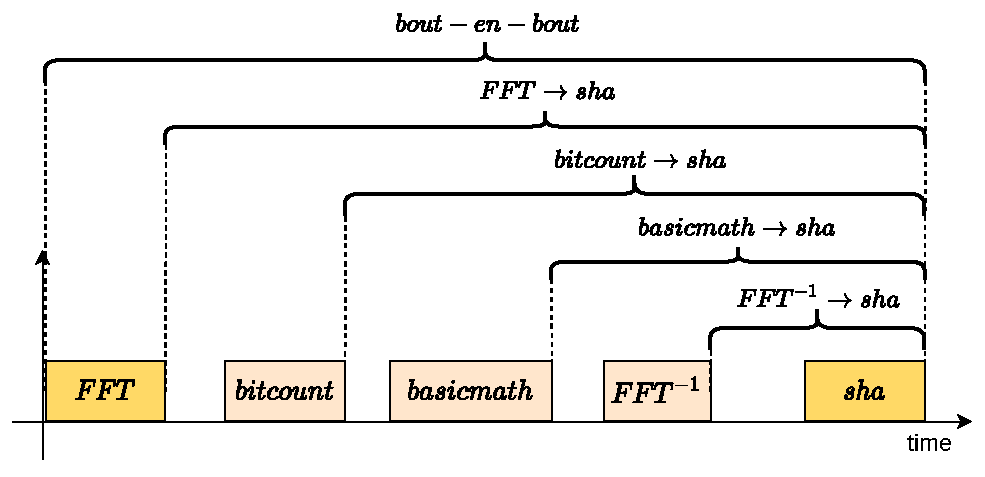
\includegraphics[width=0.8\linewidth]{schemas/mesures-rWCRT}
	\caption{Mesures des temps d'exécution restant sur une Trace d'exécution}
	\label{fig:chronogrammes-rwcrt-example}
\end{figure}

On obtient ainsi 5 mesures de temps d'exécution restant constaté pour chaque instance $p$ de la chaîne qui s'est exécuté tout du long de l'expérimentation. L'agrégation de ces données est résumée dans le~\autoref{tab:rWCRTi}. Il est alors possible de déterminer les valeurs de $rWCRT(\tau_i)$, comme étant une borne maximum du temps d'exécution des tâches restantes de la chaîne de tâche, tel qu'enregistrée par le module de surveillance.  Ainsi, les valeurs des paramètres d'anticipation $rWCRT()$ choisis sont indiqués dans la dernière colonne du~\autoref{tab:rWCRTi}.

\cmnt{
		\begin{table}[ht]
	\renewcommand{\arraystretch}{1}
	\centering
	\caption{Valeurs de $rWCRT(\tau_i)$ de la chaîne de tâches critiques en mode dégradé} \label{tab:rWCRTi}
	\begin{tabular}{@{}lrrrrr@{}}
		\toprule
		$ rWCRT$ 	& FFT 	& Bitcount & BasicMath & FFT\up{-1}		\\
		\midrule
		Temps (ms)  &  93   &    68    &   49.5    &   25 			\\
		\bottomrule
	\end{tabular}
\end{table}

\begin{align*}
	rWCRT(\texttt{FFT}) = 190~ms		\\
	rWCRT(\texttt{Bitcount}) = 122~ms		\\
	rWCRT(\texttt{BasicMath}) = 106~ms		\\
	rWCRT(\texttt{FFT\up{-1}}) = 64~ms
\end{align*}
%% Chain loops | Anticipated Misses | Missed
%%        1985 |                 27 |      2
}

\begin{table}[ht]
  	\centering
	\caption{Profil d'exécution de la chaîne de tâches critiques en mode dégradé} \label{tab:rWCRTi}
	\begin{tabular}{@{}lrrr@{}}
		\toprule
		Exécution restante  			& Temps moyen 	& Temps max	&	rWCRT()	\\ 
		\midrule
		bout-en-bout 					& 125.86~ms     & 138.26~ms	&	/		\\ 
		FFT $\rightarrow$ sha			& 103.79~ms     & 128.25~ms	&	129~ms	\\
		bitcount $\rightarrow$ sha      & 77.58~ms      &  96.61~ms	&	97~ms	\\
		basicmath $\rightarrow$ sha     & 59.82~ms      &  85.24~ms	&	86~ms	\\
		FFT\up{-1} $ \rightarrow$ sha   & 27.06~ms      &  42.91~ms	&	43~ms	\\
		\bottomrule
	\end{tabular}
\end{table}

\pagebreak
\subsubsection{Vérification du jeu de tâches complet (\ctxt{5})}

En complément de la chaîne de tâches critiques il a bien sûr fallu faire une sélection de tâches pour représenter la partie non critique du système et en fixer l'allocation sur les cœurs, les périodes d'exécution, etc.
Le choix s'est naturellement porté sur des tâches classifiées NOISE, mais aussi quelques-unes classées CLEAN tel qu'on peut le voir sur le fichier de configuration~\ref{code:tasksBE.in}~: 

\begin{lstlisting}[basicstyle=\footnotesize\ttfamily, caption={Tâches non critiques sélectionnées}, numbers=none, label={code:tasksBE.in}]
ID name            FUNC    P  T   A  ARGS
11 BE_sha_S        sha     0  80  2  < [input] > [output].txt
12 BE_susan-S_corn susan   0  80  2  -c > [input].pgm < [output].pgm
13 BE_susan-S_smoo susan   0  80  2  -s > [input].pgm < [output].pgm
14 BE_susan-S_edg  susan   0  80  2  -e > [input].pgm < [output].pgm
15 BE_cjpeg-S      cjpeg   0  30  F  -dct int -progressive -opt [...]
16 BE_gsmToast_S   toast   0  60  4  -fps -c [input].au > [output]
17 BE_gsmUToast_S  toast   0  60  4  -dfps -c [input].gsm > [output]
18 BE_bitcount_S   bitcnts 0  60  4  75000 > [output]
21 BE_sha2_S       sha     0  80  4  < [input].asc > [output].txt
22 BE_susan_S_co.  susan   0  80  1  -c [input].pgm [output].pgm
23 BE_susan_S_sm.  susan   0  80  8  -s [input].pgm [output].pgm
24 BE_susan_S_ed.  susan   0  80  8  -e [input].pgm [output].pgm
25 BE_cjpeg2_S     cjpeg   0  30  F  -dct int -progressive -opt [...]
26 BE_gsmToast2_S  toast   0  60  8  -fps -c [input].au > [output]
27 BE_gsmUToast2_S toast   0  60  8  -dfps -c [input].gsm > [output]
28 BE_bitcount2_S  bitcnts 0  60  F  75000 > [output].txt
\end{lstlisting}

En plus des informations déjà présentées précédemment sur le format d'un tel fichier de configuration, on remarquera ici la colonne de l'affinité des tâches, qui est exprimé en hexadécimal pour couvrir toutes les configurations possibles sur un processeur à 4 cœurs. Ainsi, par exemple F(hex) = 1111(binaire) donne l'affinité par défaut à l'ensemble des cœurs, tandis que 1 (=0001), 2 (=0010), 4 (=0100) et 8 (=1000) permettent un partitionnement des tâches à un cœur unique. Dans la configuration ci-présentée on a un système semi-partitionné, où la plupart des tâches sont assignées à un cœur unique tandis qu'une minorité sont libres de migrer entre tous les cœurs.

Cela nous permet de mettre en place l'étape \ctxt{5} du protocole général, où l'on exécute à la fois la chaîne de tâches critiques et les tâches non critiques, accompagnées du mécanisme de surveillance sans la partie Contrôle. On désactive pour cela l'envoi du signal de changement de mode, mais tout le reste de l'algorithme du contrôle reste actif.

Cela nous permet d'une part de mesurer l'ordonnançabilité du système ainsi déployé. On peut aussi mesurer l'empreinte du Core Control Component en termes de temps d'exécution sur le CPU. Et enfin, en provoquant des déclenchements du mode dégradé de façon forcée (option directement en dur dans le code du Core Control Component) on peut mesurer le temps de changement de mode $t_{SW}$.

Le résultat que l'on obtient sur le profil d'exécution de la chaîne de tâche est compilé dans la~\autoref{graph:taskchainavecinterference} avec la courbe \textcolor{red}{rouge}, superposée à la courbe \textcolor{blue}{bleue} précédemment obtenue. On distingue clairement la conséquence d'une quasi surcharge du système avec l'ajout des tâches non critiques, qui provoquent des interférences réelles (en opposition avec les interférences forcées artificiellement via stress-ng) sur l'exécution des tâches critiques. %partir de l'expérimentation précédente sur la chaîne de tâche, il est aussi possible d'extraire , regarding previous results from step~\ctxt{3}, we set $W_{max} = 1$ms, and $t_{sw} = 500\mu$s for our platform.

\begin{figure}[ht]
	\centering
	\scalebox{0.9}{%% Creator: Matplotlib, PGF backend
%%
%% To include the figure in your LaTeX document, write
%%   \input{<filename>.pgf}
%%
%% Make sure the required packages are loaded in your preamble
%%   \usepackage{pgf}
%%
%% and, on pdftex
%%   \usepackage[utf8]{inputenc}\DeclareUnicodeCharacter{2212}{-}
%%
%% or, on luatex and xetex
%%   \usepackage{unicode-math}
%%
%% Figures using additional raster images can only be included by \input if
%% they are in the same directory as the main LaTeX file. For loading figures
%% from other directories you can use the `import` package
%%   \usepackage{import}
%%
%% and then include the figures with
%%   \import{<path to file>}{<filename>.pgf}
%%
%% Matplotlib used the following preamble
%%   \usepackage{fontspec}
%%   \setmainfont{DejaVuSerif.ttf}[Path=/usr/local/lib/python3.6/dist-packages/matplotlib/mpl-data/fonts/ttf/]
%%   \setsansfont{DejaVuSans.ttf}[Path=/usr/local/lib/python3.6/dist-packages/matplotlib/mpl-data/fonts/ttf/]
%%   \setmonofont{DejaVuSansMono.ttf}[Path=/usr/local/lib/python3.6/dist-packages/matplotlib/mpl-data/fonts/ttf/]
%%
\begingroup%
\makeatletter%
\begin{pgfpicture}%
\pgfpathrectangle{\pgfpointorigin}{\pgfqpoint{6.400000in}{4.800000in}}%
\pgfusepath{use as bounding box, clip}%
\begin{pgfscope}%
\pgfsetbuttcap%
\pgfsetmiterjoin%
\definecolor{currentfill}{rgb}{1.000000,1.000000,1.000000}%
\pgfsetfillcolor{currentfill}%
\pgfsetlinewidth{0.000000pt}%
\definecolor{currentstroke}{rgb}{1.000000,1.000000,1.000000}%
\pgfsetstrokecolor{currentstroke}%
\pgfsetdash{}{0pt}%
\pgfpathmoveto{\pgfqpoint{0.000000in}{0.000000in}}%
\pgfpathlineto{\pgfqpoint{6.400000in}{0.000000in}}%
\pgfpathlineto{\pgfqpoint{6.400000in}{4.800000in}}%
\pgfpathlineto{\pgfqpoint{0.000000in}{4.800000in}}%
\pgfpathclose%
\pgfusepath{fill}%
\end{pgfscope}%
\begin{pgfscope}%
\pgfsetbuttcap%
\pgfsetmiterjoin%
\definecolor{currentfill}{rgb}{1.000000,1.000000,1.000000}%
\pgfsetfillcolor{currentfill}%
\pgfsetlinewidth{0.000000pt}%
\definecolor{currentstroke}{rgb}{0.000000,0.000000,0.000000}%
\pgfsetstrokecolor{currentstroke}%
\pgfsetstrokeopacity{0.000000}%
\pgfsetdash{}{0pt}%
\pgfpathmoveto{\pgfqpoint{0.800000in}{0.528000in}}%
\pgfpathlineto{\pgfqpoint{5.760000in}{0.528000in}}%
\pgfpathlineto{\pgfqpoint{5.760000in}{4.224000in}}%
\pgfpathlineto{\pgfqpoint{0.800000in}{4.224000in}}%
\pgfpathclose%
\pgfusepath{fill}%
\end{pgfscope}%
\begin{pgfscope}%
\pgfpathrectangle{\pgfqpoint{0.800000in}{0.528000in}}{\pgfqpoint{4.960000in}{3.696000in}}%
\pgfusepath{clip}%
\pgfsetroundcap%
\pgfsetroundjoin%
\pgfsetlinewidth{1.003750pt}%
\definecolor{currentstroke}{rgb}{0.800000,0.800000,0.800000}%
\pgfsetstrokecolor{currentstroke}%
\pgfsetdash{}{0pt}%
\pgfpathmoveto{\pgfqpoint{0.982991in}{0.528000in}}%
\pgfpathlineto{\pgfqpoint{0.982991in}{4.224000in}}%
\pgfusepath{stroke}%
\end{pgfscope}%
\begin{pgfscope}%
\definecolor{textcolor}{rgb}{0.150000,0.150000,0.150000}%
\pgfsetstrokecolor{textcolor}%
\pgfsetfillcolor{textcolor}%
\pgftext[x=0.982991in,y=0.396056in,,top]{\color{textcolor}\sffamily\fontsize{11.000000}{13.200000}\selectfont 80}%
\end{pgfscope}%
\begin{pgfscope}%
\pgfpathrectangle{\pgfqpoint{0.800000in}{0.528000in}}{\pgfqpoint{4.960000in}{3.696000in}}%
\pgfusepath{clip}%
\pgfsetroundcap%
\pgfsetroundjoin%
\pgfsetlinewidth{1.003750pt}%
\definecolor{currentstroke}{rgb}{0.800000,0.800000,0.800000}%
\pgfsetstrokecolor{currentstroke}%
\pgfsetdash{}{0pt}%
\pgfpathmoveto{\pgfqpoint{1.564331in}{0.528000in}}%
\pgfpathlineto{\pgfqpoint{1.564331in}{4.224000in}}%
\pgfusepath{stroke}%
\end{pgfscope}%
\begin{pgfscope}%
\definecolor{textcolor}{rgb}{0.150000,0.150000,0.150000}%
\pgfsetstrokecolor{textcolor}%
\pgfsetfillcolor{textcolor}%
\pgftext[x=1.564331in,y=0.396056in,,top]{\color{textcolor}\sffamily\fontsize{11.000000}{13.200000}\selectfont 100}%
\end{pgfscope}%
\begin{pgfscope}%
\pgfpathrectangle{\pgfqpoint{0.800000in}{0.528000in}}{\pgfqpoint{4.960000in}{3.696000in}}%
\pgfusepath{clip}%
\pgfsetroundcap%
\pgfsetroundjoin%
\pgfsetlinewidth{1.003750pt}%
\definecolor{currentstroke}{rgb}{0.800000,0.800000,0.800000}%
\pgfsetstrokecolor{currentstroke}%
\pgfsetdash{}{0pt}%
\pgfpathmoveto{\pgfqpoint{2.145672in}{0.528000in}}%
\pgfpathlineto{\pgfqpoint{2.145672in}{4.224000in}}%
\pgfusepath{stroke}%
\end{pgfscope}%
\begin{pgfscope}%
\definecolor{textcolor}{rgb}{0.150000,0.150000,0.150000}%
\pgfsetstrokecolor{textcolor}%
\pgfsetfillcolor{textcolor}%
\pgftext[x=2.145672in,y=0.396056in,,top]{\color{textcolor}\sffamily\fontsize{11.000000}{13.200000}\selectfont 120}%
\end{pgfscope}%
\begin{pgfscope}%
\pgfpathrectangle{\pgfqpoint{0.800000in}{0.528000in}}{\pgfqpoint{4.960000in}{3.696000in}}%
\pgfusepath{clip}%
\pgfsetroundcap%
\pgfsetroundjoin%
\pgfsetlinewidth{1.003750pt}%
\definecolor{currentstroke}{rgb}{0.800000,0.800000,0.800000}%
\pgfsetstrokecolor{currentstroke}%
\pgfsetdash{}{0pt}%
\pgfpathmoveto{\pgfqpoint{2.727012in}{0.528000in}}%
\pgfpathlineto{\pgfqpoint{2.727012in}{4.224000in}}%
\pgfusepath{stroke}%
\end{pgfscope}%
\begin{pgfscope}%
\definecolor{textcolor}{rgb}{0.150000,0.150000,0.150000}%
\pgfsetstrokecolor{textcolor}%
\pgfsetfillcolor{textcolor}%
\pgftext[x=2.727012in,y=0.396056in,,top]{\color{textcolor}\sffamily\fontsize{11.000000}{13.200000}\selectfont 140}%
\end{pgfscope}%
\begin{pgfscope}%
\pgfpathrectangle{\pgfqpoint{0.800000in}{0.528000in}}{\pgfqpoint{4.960000in}{3.696000in}}%
\pgfusepath{clip}%
\pgfsetroundcap%
\pgfsetroundjoin%
\pgfsetlinewidth{1.003750pt}%
\definecolor{currentstroke}{rgb}{0.800000,0.800000,0.800000}%
\pgfsetstrokecolor{currentstroke}%
\pgfsetdash{}{0pt}%
\pgfpathmoveto{\pgfqpoint{3.308352in}{0.528000in}}%
\pgfpathlineto{\pgfqpoint{3.308352in}{4.224000in}}%
\pgfusepath{stroke}%
\end{pgfscope}%
\begin{pgfscope}%
\definecolor{textcolor}{rgb}{0.150000,0.150000,0.150000}%
\pgfsetstrokecolor{textcolor}%
\pgfsetfillcolor{textcolor}%
\pgftext[x=3.308352in,y=0.396056in,,top]{\color{textcolor}\sffamily\fontsize{11.000000}{13.200000}\selectfont 160}%
\end{pgfscope}%
\begin{pgfscope}%
\pgfpathrectangle{\pgfqpoint{0.800000in}{0.528000in}}{\pgfqpoint{4.960000in}{3.696000in}}%
\pgfusepath{clip}%
\pgfsetroundcap%
\pgfsetroundjoin%
\pgfsetlinewidth{1.003750pt}%
\definecolor{currentstroke}{rgb}{0.800000,0.800000,0.800000}%
\pgfsetstrokecolor{currentstroke}%
\pgfsetdash{}{0pt}%
\pgfpathmoveto{\pgfqpoint{3.889692in}{0.528000in}}%
\pgfpathlineto{\pgfqpoint{3.889692in}{4.224000in}}%
\pgfusepath{stroke}%
\end{pgfscope}%
\begin{pgfscope}%
\definecolor{textcolor}{rgb}{0.150000,0.150000,0.150000}%
\pgfsetstrokecolor{textcolor}%
\pgfsetfillcolor{textcolor}%
\pgftext[x=3.889692in,y=0.396056in,,top]{\color{textcolor}\sffamily\fontsize{11.000000}{13.200000}\selectfont 180}%
\end{pgfscope}%
\begin{pgfscope}%
\pgfpathrectangle{\pgfqpoint{0.800000in}{0.528000in}}{\pgfqpoint{4.960000in}{3.696000in}}%
\pgfusepath{clip}%
\pgfsetroundcap%
\pgfsetroundjoin%
\pgfsetlinewidth{1.003750pt}%
\definecolor{currentstroke}{rgb}{0.800000,0.800000,0.800000}%
\pgfsetstrokecolor{currentstroke}%
\pgfsetdash{}{0pt}%
\pgfpathmoveto{\pgfqpoint{4.471032in}{0.528000in}}%
\pgfpathlineto{\pgfqpoint{4.471032in}{4.224000in}}%
\pgfusepath{stroke}%
\end{pgfscope}%
\begin{pgfscope}%
\definecolor{textcolor}{rgb}{0.150000,0.150000,0.150000}%
\pgfsetstrokecolor{textcolor}%
\pgfsetfillcolor{textcolor}%
\pgftext[x=4.471032in,y=0.396056in,,top]{\color{textcolor}\sffamily\fontsize{11.000000}{13.200000}\selectfont 200}%
\end{pgfscope}%
\begin{pgfscope}%
\pgfpathrectangle{\pgfqpoint{0.800000in}{0.528000in}}{\pgfqpoint{4.960000in}{3.696000in}}%
\pgfusepath{clip}%
\pgfsetroundcap%
\pgfsetroundjoin%
\pgfsetlinewidth{1.003750pt}%
\definecolor{currentstroke}{rgb}{0.800000,0.800000,0.800000}%
\pgfsetstrokecolor{currentstroke}%
\pgfsetdash{}{0pt}%
\pgfpathmoveto{\pgfqpoint{5.052373in}{0.528000in}}%
\pgfpathlineto{\pgfqpoint{5.052373in}{4.224000in}}%
\pgfusepath{stroke}%
\end{pgfscope}%
\begin{pgfscope}%
\definecolor{textcolor}{rgb}{0.150000,0.150000,0.150000}%
\pgfsetstrokecolor{textcolor}%
\pgfsetfillcolor{textcolor}%
\pgftext[x=5.052373in,y=0.396056in,,top]{\color{textcolor}\sffamily\fontsize{11.000000}{13.200000}\selectfont 220}%
\end{pgfscope}%
\begin{pgfscope}%
\pgfpathrectangle{\pgfqpoint{0.800000in}{0.528000in}}{\pgfqpoint{4.960000in}{3.696000in}}%
\pgfusepath{clip}%
\pgfsetroundcap%
\pgfsetroundjoin%
\pgfsetlinewidth{1.003750pt}%
\definecolor{currentstroke}{rgb}{0.800000,0.800000,0.800000}%
\pgfsetstrokecolor{currentstroke}%
\pgfsetdash{}{0pt}%
\pgfpathmoveto{\pgfqpoint{5.633713in}{0.528000in}}%
\pgfpathlineto{\pgfqpoint{5.633713in}{4.224000in}}%
\pgfusepath{stroke}%
\end{pgfscope}%
\begin{pgfscope}%
\definecolor{textcolor}{rgb}{0.150000,0.150000,0.150000}%
\pgfsetstrokecolor{textcolor}%
\pgfsetfillcolor{textcolor}%
\pgftext[x=5.633713in,y=0.396056in,,top]{\color{textcolor}\sffamily\fontsize{11.000000}{13.200000}\selectfont 240}%
\end{pgfscope}%
\begin{pgfscope}%
\definecolor{textcolor}{rgb}{0.150000,0.150000,0.150000}%
\pgfsetstrokecolor{textcolor}%
\pgfsetfillcolor{textcolor}%
\pgftext[x=3.280000in,y=0.192646in,,top]{\color{textcolor}\sffamily\fontsize{12.000000}{14.400000}\selectfont Temps de réponse bout-en-bout (ms)}%
\end{pgfscope}%
\begin{pgfscope}%
\pgfpathrectangle{\pgfqpoint{0.800000in}{0.528000in}}{\pgfqpoint{4.960000in}{3.696000in}}%
\pgfusepath{clip}%
\pgfsetroundcap%
\pgfsetroundjoin%
\pgfsetlinewidth{1.003750pt}%
\definecolor{currentstroke}{rgb}{0.800000,0.800000,0.800000}%
\pgfsetstrokecolor{currentstroke}%
\pgfsetdash{}{0pt}%
\pgfpathmoveto{\pgfqpoint{0.800000in}{0.528000in}}%
\pgfpathlineto{\pgfqpoint{5.760000in}{0.528000in}}%
\pgfusepath{stroke}%
\end{pgfscope}%
\begin{pgfscope}%
\definecolor{textcolor}{rgb}{0.150000,0.150000,0.150000}%
\pgfsetstrokecolor{textcolor}%
\pgfsetfillcolor{textcolor}%
\pgftext[x=0.527886in, y=0.469962in, left, base]{\color{textcolor}\sffamily\fontsize{11.000000}{13.200000}\selectfont 0}%
\end{pgfscope}%
\begin{pgfscope}%
\pgfpathrectangle{\pgfqpoint{0.800000in}{0.528000in}}{\pgfqpoint{4.960000in}{3.696000in}}%
\pgfusepath{clip}%
\pgfsetroundcap%
\pgfsetroundjoin%
\pgfsetlinewidth{1.003750pt}%
\definecolor{currentstroke}{rgb}{0.800000,0.800000,0.800000}%
\pgfsetstrokecolor{currentstroke}%
\pgfsetdash{}{0pt}%
\pgfpathmoveto{\pgfqpoint{0.800000in}{1.274913in}}%
\pgfpathlineto{\pgfqpoint{5.760000in}{1.274913in}}%
\pgfusepath{stroke}%
\end{pgfscope}%
\begin{pgfscope}%
\definecolor{textcolor}{rgb}{0.150000,0.150000,0.150000}%
\pgfsetstrokecolor{textcolor}%
\pgfsetfillcolor{textcolor}%
\pgftext[x=0.527886in, y=1.216875in, left, base]{\color{textcolor}\sffamily\fontsize{11.000000}{13.200000}\selectfont 2\%}%
\end{pgfscope}%
\begin{pgfscope}%
\pgfpathrectangle{\pgfqpoint{0.800000in}{0.528000in}}{\pgfqpoint{4.960000in}{3.696000in}}%
\pgfusepath{clip}%
\pgfsetroundcap%
\pgfsetroundjoin%
\pgfsetlinewidth{1.003750pt}%
\definecolor{currentstroke}{rgb}{0.800000,0.800000,0.800000}%
\pgfsetstrokecolor{currentstroke}%
\pgfsetdash{}{0pt}%
\pgfpathmoveto{\pgfqpoint{0.800000in}{2.021825in}}%
\pgfpathlineto{\pgfqpoint{5.760000in}{2.021825in}}%
\pgfusepath{stroke}%
\end{pgfscope}%
\begin{pgfscope}%
\definecolor{textcolor}{rgb}{0.150000,0.150000,0.150000}%
\pgfsetstrokecolor{textcolor}%
\pgfsetfillcolor{textcolor}%
\pgftext[x=0.527886in, y=1.963788in, left, base]{\color{textcolor}\sffamily\fontsize{11.000000}{13.200000}\selectfont 4\%}%
\end{pgfscope}%
\begin{pgfscope}%
\pgfpathrectangle{\pgfqpoint{0.800000in}{0.528000in}}{\pgfqpoint{4.960000in}{3.696000in}}%
\pgfusepath{clip}%
\pgfsetroundcap%
\pgfsetroundjoin%
\pgfsetlinewidth{1.003750pt}%
\definecolor{currentstroke}{rgb}{0.800000,0.800000,0.800000}%
\pgfsetstrokecolor{currentstroke}%
\pgfsetdash{}{0pt}%
\pgfpathmoveto{\pgfqpoint{0.800000in}{2.768738in}}%
\pgfpathlineto{\pgfqpoint{5.760000in}{2.768738in}}%
\pgfusepath{stroke}%
\end{pgfscope}%
\begin{pgfscope}%
\definecolor{textcolor}{rgb}{0.150000,0.150000,0.150000}%
\pgfsetstrokecolor{textcolor}%
\pgfsetfillcolor{textcolor}%
\pgftext[x=0.527886in, y=2.710700in, left, base]{\color{textcolor}\sffamily\fontsize{11.000000}{13.200000}\selectfont 6\%}%
\end{pgfscope}%
\begin{pgfscope}%
\pgfpathrectangle{\pgfqpoint{0.800000in}{0.528000in}}{\pgfqpoint{4.960000in}{3.696000in}}%
\pgfusepath{clip}%
\pgfsetroundcap%
\pgfsetroundjoin%
\pgfsetlinewidth{1.003750pt}%
\definecolor{currentstroke}{rgb}{0.800000,0.800000,0.800000}%
\pgfsetstrokecolor{currentstroke}%
\pgfsetdash{}{0pt}%
\pgfpathmoveto{\pgfqpoint{0.800000in}{3.515650in}}%
\pgfpathlineto{\pgfqpoint{5.760000in}{3.515650in}}%
\pgfusepath{stroke}%
\end{pgfscope}%
\begin{pgfscope}%
\definecolor{textcolor}{rgb}{0.150000,0.150000,0.150000}%
\pgfsetstrokecolor{textcolor}%
\pgfsetfillcolor{textcolor}%
\pgftext[x=0.527886in, y=3.457613in, left, base]{\color{textcolor}\sffamily\fontsize{11.000000}{13.200000}\selectfont 8\%}%
\end{pgfscope}%
\begin{pgfscope}%
\definecolor{textcolor}{rgb}{0.150000,0.150000,0.150000}%
\pgfsetstrokecolor{textcolor}%
\pgfsetfillcolor{textcolor}%
\pgftext[x=0.272331in,y=2.376000in,,bottom,rotate=90.000000]{\color{textcolor}\sffamily\fontsize{12.000000}{14.400000}\selectfont Densité de distribution}%
\end{pgfscope}%

\begin{pgfscope}%
\pgfpathrectangle{\pgfqpoint{0.800000in}{0.528000in}}{\pgfqpoint{4.960000in}{3.696000in}}%
\pgfusepath{clip}%
\pgfsetbuttcap%
\pgfsetroundjoin%
\definecolor{currentfill}{rgb}{0.018039,0.067059,0.550196}%
\pgfsetfillcolor{currentfill}%
\pgfsetfillopacity{0.250000}%
\pgfsetlinewidth{1.003750pt}%
\definecolor{currentstroke}{rgb}{0.018039,0.067059,0.550196}%
\pgfsetstrokecolor{currentstroke}%
\pgfsetdash{}{0pt}%
\pgfsys@defobject{currentmarker}{\pgfqpoint{1.025455in}{0.528000in}}{\pgfqpoint{2.674537in}{2.186749in}}{%
\pgfpathmoveto{\pgfqpoint{1.025455in}{0.529344in}}%
\pgfpathlineto{\pgfqpoint{1.025455in}{0.528000in}}%
\pgfpathlineto{\pgfqpoint{1.033741in}{0.528000in}}%
\pgfpathlineto{\pgfqpoint{1.042028in}{0.528000in}}%
\pgfpathlineto{\pgfqpoint{1.050315in}{0.528000in}}%
\pgfpathlineto{\pgfqpoint{1.058602in}{0.528000in}}%
\pgfpathlineto{\pgfqpoint{1.066889in}{0.528000in}}%
\pgfpathlineto{\pgfqpoint{1.075176in}{0.528000in}}%
\pgfpathlineto{\pgfqpoint{1.083462in}{0.528000in}}%
\pgfpathlineto{\pgfqpoint{1.091749in}{0.528000in}}%
\pgfpathlineto{\pgfqpoint{1.100036in}{0.528000in}}%
\pgfpathlineto{\pgfqpoint{1.108323in}{0.528000in}}%
\pgfpathlineto{\pgfqpoint{1.116610in}{0.528000in}}%
\pgfpathlineto{\pgfqpoint{1.124897in}{0.528000in}}%
\pgfpathlineto{\pgfqpoint{1.133184in}{0.528000in}}%
\pgfpathlineto{\pgfqpoint{1.141470in}{0.528000in}}%
\pgfpathlineto{\pgfqpoint{1.149757in}{0.528000in}}%
\pgfpathlineto{\pgfqpoint{1.158044in}{0.528000in}}%
\pgfpathlineto{\pgfqpoint{1.166331in}{0.528000in}}%
\pgfpathlineto{\pgfqpoint{1.174618in}{0.528000in}}%
\pgfpathlineto{\pgfqpoint{1.182905in}{0.528000in}}%
\pgfpathlineto{\pgfqpoint{1.191191in}{0.528000in}}%
\pgfpathlineto{\pgfqpoint{1.199478in}{0.528000in}}%
\pgfpathlineto{\pgfqpoint{1.207765in}{0.528000in}}%
\pgfpathlineto{\pgfqpoint{1.216052in}{0.528000in}}%
\pgfpathlineto{\pgfqpoint{1.224339in}{0.528000in}}%
\pgfpathlineto{\pgfqpoint{1.232626in}{0.528000in}}%
\pgfpathlineto{\pgfqpoint{1.240913in}{0.528000in}}%
\pgfpathlineto{\pgfqpoint{1.249199in}{0.528000in}}%
\pgfpathlineto{\pgfqpoint{1.257486in}{0.528000in}}%
\pgfpathlineto{\pgfqpoint{1.265773in}{0.528000in}}%
\pgfpathlineto{\pgfqpoint{1.274060in}{0.528000in}}%
\pgfpathlineto{\pgfqpoint{1.282347in}{0.528000in}}%
\pgfpathlineto{\pgfqpoint{1.290634in}{0.528000in}}%
\pgfpathlineto{\pgfqpoint{1.298920in}{0.528000in}}%
\pgfpathlineto{\pgfqpoint{1.307207in}{0.528000in}}%
\pgfpathlineto{\pgfqpoint{1.315494in}{0.528000in}}%
\pgfpathlineto{\pgfqpoint{1.323781in}{0.528000in}}%
\pgfpathlineto{\pgfqpoint{1.332068in}{0.528000in}}%
\pgfpathlineto{\pgfqpoint{1.340355in}{0.528000in}}%
\pgfpathlineto{\pgfqpoint{1.348642in}{0.528000in}}%
\pgfpathlineto{\pgfqpoint{1.356928in}{0.528000in}}%
\pgfpathlineto{\pgfqpoint{1.365215in}{0.528000in}}%
\pgfpathlineto{\pgfqpoint{1.373502in}{0.528000in}}%
\pgfpathlineto{\pgfqpoint{1.381789in}{0.528000in}}%
\pgfpathlineto{\pgfqpoint{1.390076in}{0.528000in}}%
\pgfpathlineto{\pgfqpoint{1.398363in}{0.528000in}}%
\pgfpathlineto{\pgfqpoint{1.406650in}{0.528000in}}%
\pgfpathlineto{\pgfqpoint{1.414936in}{0.528000in}}%
\pgfpathlineto{\pgfqpoint{1.423223in}{0.528000in}}%
\pgfpathlineto{\pgfqpoint{1.431510in}{0.528000in}}%
\pgfpathlineto{\pgfqpoint{1.439797in}{0.528000in}}%
\pgfpathlineto{\pgfqpoint{1.448084in}{0.528000in}}%
\pgfpathlineto{\pgfqpoint{1.456371in}{0.528000in}}%
\pgfpathlineto{\pgfqpoint{1.464657in}{0.528000in}}%
\pgfpathlineto{\pgfqpoint{1.472944in}{0.528000in}}%
\pgfpathlineto{\pgfqpoint{1.481231in}{0.528000in}}%
\pgfpathlineto{\pgfqpoint{1.489518in}{0.528000in}}%
\pgfpathlineto{\pgfqpoint{1.497805in}{0.528000in}}%
\pgfpathlineto{\pgfqpoint{1.506092in}{0.528000in}}%
\pgfpathlineto{\pgfqpoint{1.514379in}{0.528000in}}%
\pgfpathlineto{\pgfqpoint{1.522665in}{0.528000in}}%
\pgfpathlineto{\pgfqpoint{1.530952in}{0.528000in}}%
\pgfpathlineto{\pgfqpoint{1.539239in}{0.528000in}}%
\pgfpathlineto{\pgfqpoint{1.547526in}{0.528000in}}%
\pgfpathlineto{\pgfqpoint{1.555813in}{0.528000in}}%
\pgfpathlineto{\pgfqpoint{1.564100in}{0.528000in}}%
\pgfpathlineto{\pgfqpoint{1.572386in}{0.528000in}}%
\pgfpathlineto{\pgfqpoint{1.580673in}{0.528000in}}%
\pgfpathlineto{\pgfqpoint{1.588960in}{0.528000in}}%
\pgfpathlineto{\pgfqpoint{1.597247in}{0.528000in}}%
\pgfpathlineto{\pgfqpoint{1.605534in}{0.528000in}}%
\pgfpathlineto{\pgfqpoint{1.613821in}{0.528000in}}%
\pgfpathlineto{\pgfqpoint{1.622108in}{0.528000in}}%
\pgfpathlineto{\pgfqpoint{1.630394in}{0.528000in}}%
\pgfpathlineto{\pgfqpoint{1.638681in}{0.528000in}}%
\pgfpathlineto{\pgfqpoint{1.646968in}{0.528000in}}%
\pgfpathlineto{\pgfqpoint{1.655255in}{0.528000in}}%
\pgfpathlineto{\pgfqpoint{1.663542in}{0.528000in}}%
\pgfpathlineto{\pgfqpoint{1.671829in}{0.528000in}}%
\pgfpathlineto{\pgfqpoint{1.680115in}{0.528000in}}%
\pgfpathlineto{\pgfqpoint{1.688402in}{0.528000in}}%
\pgfpathlineto{\pgfqpoint{1.696689in}{0.528000in}}%
\pgfpathlineto{\pgfqpoint{1.704976in}{0.528000in}}%
\pgfpathlineto{\pgfqpoint{1.713263in}{0.528000in}}%
\pgfpathlineto{\pgfqpoint{1.721550in}{0.528000in}}%
\pgfpathlineto{\pgfqpoint{1.729837in}{0.528000in}}%
\pgfpathlineto{\pgfqpoint{1.738123in}{0.528000in}}%
\pgfpathlineto{\pgfqpoint{1.746410in}{0.528000in}}%
\pgfpathlineto{\pgfqpoint{1.754697in}{0.528000in}}%
\pgfpathlineto{\pgfqpoint{1.762984in}{0.528000in}}%
\pgfpathlineto{\pgfqpoint{1.771271in}{0.528000in}}%
\pgfpathlineto{\pgfqpoint{1.779558in}{0.528000in}}%
\pgfpathlineto{\pgfqpoint{1.787844in}{0.528000in}}%
\pgfpathlineto{\pgfqpoint{1.796131in}{0.528000in}}%
\pgfpathlineto{\pgfqpoint{1.804418in}{0.528000in}}%
\pgfpathlineto{\pgfqpoint{1.812705in}{0.528000in}}%
\pgfpathlineto{\pgfqpoint{1.820992in}{0.528000in}}%
\pgfpathlineto{\pgfqpoint{1.829279in}{0.528000in}}%
\pgfpathlineto{\pgfqpoint{1.837566in}{0.528000in}}%
\pgfpathlineto{\pgfqpoint{1.845852in}{0.528000in}}%
\pgfpathlineto{\pgfqpoint{1.854139in}{0.528000in}}%
\pgfpathlineto{\pgfqpoint{1.862426in}{0.528000in}}%
\pgfpathlineto{\pgfqpoint{1.870713in}{0.528000in}}%
\pgfpathlineto{\pgfqpoint{1.879000in}{0.528000in}}%
\pgfpathlineto{\pgfqpoint{1.887287in}{0.528000in}}%
\pgfpathlineto{\pgfqpoint{1.895573in}{0.528000in}}%
\pgfpathlineto{\pgfqpoint{1.903860in}{0.528000in}}%
\pgfpathlineto{\pgfqpoint{1.912147in}{0.528000in}}%
\pgfpathlineto{\pgfqpoint{1.920434in}{0.528000in}}%
\pgfpathlineto{\pgfqpoint{1.928721in}{0.528000in}}%
\pgfpathlineto{\pgfqpoint{1.937008in}{0.528000in}}%
\pgfpathlineto{\pgfqpoint{1.945295in}{0.528000in}}%
\pgfpathlineto{\pgfqpoint{1.953581in}{0.528000in}}%
\pgfpathlineto{\pgfqpoint{1.961868in}{0.528000in}}%
\pgfpathlineto{\pgfqpoint{1.970155in}{0.528000in}}%
\pgfpathlineto{\pgfqpoint{1.978442in}{0.528000in}}%
\pgfpathlineto{\pgfqpoint{1.986729in}{0.528000in}}%
\pgfpathlineto{\pgfqpoint{1.995016in}{0.528000in}}%
\pgfpathlineto{\pgfqpoint{2.003302in}{0.528000in}}%
\pgfpathlineto{\pgfqpoint{2.011589in}{0.528000in}}%
\pgfpathlineto{\pgfqpoint{2.019876in}{0.528000in}}%
\pgfpathlineto{\pgfqpoint{2.028163in}{0.528000in}}%
\pgfpathlineto{\pgfqpoint{2.036450in}{0.528000in}}%
\pgfpathlineto{\pgfqpoint{2.044737in}{0.528000in}}%
\pgfpathlineto{\pgfqpoint{2.053024in}{0.528000in}}%
\pgfpathlineto{\pgfqpoint{2.061310in}{0.528000in}}%
\pgfpathlineto{\pgfqpoint{2.069597in}{0.528000in}}%
\pgfpathlineto{\pgfqpoint{2.077884in}{0.528000in}}%
\pgfpathlineto{\pgfqpoint{2.086171in}{0.528000in}}%
\pgfpathlineto{\pgfqpoint{2.094458in}{0.528000in}}%
\pgfpathlineto{\pgfqpoint{2.102745in}{0.528000in}}%
\pgfpathlineto{\pgfqpoint{2.111032in}{0.528000in}}%
\pgfpathlineto{\pgfqpoint{2.119318in}{0.528000in}}%
\pgfpathlineto{\pgfqpoint{2.127605in}{0.528000in}}%
\pgfpathlineto{\pgfqpoint{2.135892in}{0.528000in}}%
\pgfpathlineto{\pgfqpoint{2.144179in}{0.528000in}}%
\pgfpathlineto{\pgfqpoint{2.152466in}{0.528000in}}%
\pgfpathlineto{\pgfqpoint{2.160753in}{0.528000in}}%
\pgfpathlineto{\pgfqpoint{2.169039in}{0.528000in}}%
\pgfpathlineto{\pgfqpoint{2.177326in}{0.528000in}}%
\pgfpathlineto{\pgfqpoint{2.185613in}{0.528000in}}%
\pgfpathlineto{\pgfqpoint{2.193900in}{0.528000in}}%
\pgfpathlineto{\pgfqpoint{2.202187in}{0.528000in}}%
\pgfpathlineto{\pgfqpoint{2.210474in}{0.528000in}}%
\pgfpathlineto{\pgfqpoint{2.218761in}{0.528000in}}%
\pgfpathlineto{\pgfqpoint{2.227047in}{0.528000in}}%
\pgfpathlineto{\pgfqpoint{2.235334in}{0.528000in}}%
\pgfpathlineto{\pgfqpoint{2.243621in}{0.528000in}}%
\pgfpathlineto{\pgfqpoint{2.251908in}{0.528000in}}%
\pgfpathlineto{\pgfqpoint{2.260195in}{0.528000in}}%
\pgfpathlineto{\pgfqpoint{2.268482in}{0.528000in}}%
\pgfpathlineto{\pgfqpoint{2.276768in}{0.528000in}}%
\pgfpathlineto{\pgfqpoint{2.285055in}{0.528000in}}%
\pgfpathlineto{\pgfqpoint{2.293342in}{0.528000in}}%
\pgfpathlineto{\pgfqpoint{2.301629in}{0.528000in}}%
\pgfpathlineto{\pgfqpoint{2.309916in}{0.528000in}}%
\pgfpathlineto{\pgfqpoint{2.318203in}{0.528000in}}%
\pgfpathlineto{\pgfqpoint{2.326490in}{0.528000in}}%
\pgfpathlineto{\pgfqpoint{2.334776in}{0.528000in}}%
\pgfpathlineto{\pgfqpoint{2.343063in}{0.528000in}}%
\pgfpathlineto{\pgfqpoint{2.351350in}{0.528000in}}%
\pgfpathlineto{\pgfqpoint{2.359637in}{0.528000in}}%
\pgfpathlineto{\pgfqpoint{2.367924in}{0.528000in}}%
\pgfpathlineto{\pgfqpoint{2.376211in}{0.528000in}}%
\pgfpathlineto{\pgfqpoint{2.384497in}{0.528000in}}%
\pgfpathlineto{\pgfqpoint{2.392784in}{0.528000in}}%
\pgfpathlineto{\pgfqpoint{2.401071in}{0.528000in}}%
\pgfpathlineto{\pgfqpoint{2.409358in}{0.528000in}}%
\pgfpathlineto{\pgfqpoint{2.417645in}{0.528000in}}%
\pgfpathlineto{\pgfqpoint{2.425932in}{0.528000in}}%
\pgfpathlineto{\pgfqpoint{2.434219in}{0.528000in}}%
\pgfpathlineto{\pgfqpoint{2.442505in}{0.528000in}}%
\pgfpathlineto{\pgfqpoint{2.450792in}{0.528000in}}%
\pgfpathlineto{\pgfqpoint{2.459079in}{0.528000in}}%
\pgfpathlineto{\pgfqpoint{2.467366in}{0.528000in}}%
\pgfpathlineto{\pgfqpoint{2.475653in}{0.528000in}}%
\pgfpathlineto{\pgfqpoint{2.483940in}{0.528000in}}%
\pgfpathlineto{\pgfqpoint{2.492226in}{0.528000in}}%
\pgfpathlineto{\pgfqpoint{2.500513in}{0.528000in}}%
\pgfpathlineto{\pgfqpoint{2.508800in}{0.528000in}}%
\pgfpathlineto{\pgfqpoint{2.517087in}{0.528000in}}%
\pgfpathlineto{\pgfqpoint{2.525374in}{0.528000in}}%
\pgfpathlineto{\pgfqpoint{2.533661in}{0.528000in}}%
\pgfpathlineto{\pgfqpoint{2.541948in}{0.528000in}}%
\pgfpathlineto{\pgfqpoint{2.550234in}{0.528000in}}%
\pgfpathlineto{\pgfqpoint{2.558521in}{0.528000in}}%
\pgfpathlineto{\pgfqpoint{2.566808in}{0.528000in}}%
\pgfpathlineto{\pgfqpoint{2.575095in}{0.528000in}}%
\pgfpathlineto{\pgfqpoint{2.583382in}{0.528000in}}%
\pgfpathlineto{\pgfqpoint{2.591669in}{0.528000in}}%
\pgfpathlineto{\pgfqpoint{2.599955in}{0.528000in}}%
\pgfpathlineto{\pgfqpoint{2.608242in}{0.528000in}}%
\pgfpathlineto{\pgfqpoint{2.616529in}{0.528000in}}%
\pgfpathlineto{\pgfqpoint{2.624816in}{0.528000in}}%
\pgfpathlineto{\pgfqpoint{2.633103in}{0.528000in}}%
\pgfpathlineto{\pgfqpoint{2.641390in}{0.528000in}}%
\pgfpathlineto{\pgfqpoint{2.649677in}{0.528000in}}%
\pgfpathlineto{\pgfqpoint{2.657963in}{0.528000in}}%
\pgfpathlineto{\pgfqpoint{2.666250in}{0.528000in}}%
\pgfpathlineto{\pgfqpoint{2.674537in}{0.528000in}}%
\pgfpathlineto{\pgfqpoint{2.674537in}{0.542142in}}%
\pgfpathlineto{\pgfqpoint{2.674537in}{0.542142in}}%
\pgfpathlineto{\pgfqpoint{2.666250in}{0.546986in}}%
\pgfpathlineto{\pgfqpoint{2.657963in}{0.553248in}}%
\pgfpathlineto{\pgfqpoint{2.649677in}{0.561258in}}%
\pgfpathlineto{\pgfqpoint{2.641390in}{0.571396in}}%
\pgfpathlineto{\pgfqpoint{2.633103in}{0.584088in}}%
\pgfpathlineto{\pgfqpoint{2.624816in}{0.599809in}}%
\pgfpathlineto{\pgfqpoint{2.616529in}{0.619069in}}%
\pgfpathlineto{\pgfqpoint{2.608242in}{0.642407in}}%
\pgfpathlineto{\pgfqpoint{2.599955in}{0.670372in}}%
\pgfpathlineto{\pgfqpoint{2.591669in}{0.703507in}}%
\pgfpathlineto{\pgfqpoint{2.583382in}{0.742320in}}%
\pgfpathlineto{\pgfqpoint{2.575095in}{0.787261in}}%
\pgfpathlineto{\pgfqpoint{2.566808in}{0.838687in}}%
\pgfpathlineto{\pgfqpoint{2.558521in}{0.896830in}}%
\pgfpathlineto{\pgfqpoint{2.550234in}{0.961761in}}%
\pgfpathlineto{\pgfqpoint{2.541948in}{1.033365in}}%
\pgfpathlineto{\pgfqpoint{2.533661in}{1.111306in}}%
\pgfpathlineto{\pgfqpoint{2.525374in}{1.195010in}}%
\pgfpathlineto{\pgfqpoint{2.517087in}{1.283650in}}%
\pgfpathlineto{\pgfqpoint{2.508800in}{1.376149in}}%
\pgfpathlineto{\pgfqpoint{2.500513in}{1.471181in}}%
\pgfpathlineto{\pgfqpoint{2.492226in}{1.567204in}}%
\pgfpathlineto{\pgfqpoint{2.483940in}{1.662490in}}%
\pgfpathlineto{\pgfqpoint{2.475653in}{1.755177in}}%
\pgfpathlineto{\pgfqpoint{2.467366in}{1.843325in}}%
\pgfpathlineto{\pgfqpoint{2.459079in}{1.924989in}}%
\pgfpathlineto{\pgfqpoint{2.450792in}{1.998285in}}%
\pgfpathlineto{\pgfqpoint{2.442505in}{2.061470in}}%
\pgfpathlineto{\pgfqpoint{2.434219in}{2.113007in}}%
\pgfpathlineto{\pgfqpoint{2.425932in}{2.151632in}}%
\pgfpathlineto{\pgfqpoint{2.417645in}{2.176405in}}%
\pgfpathlineto{\pgfqpoint{2.409358in}{2.186749in}}%
\pgfpathlineto{\pgfqpoint{2.401071in}{2.182472in}}%
\pgfpathlineto{\pgfqpoint{2.392784in}{2.163773in}}%
\pgfpathlineto{\pgfqpoint{2.384497in}{2.131229in}}%
\pgfpathlineto{\pgfqpoint{2.376211in}{2.085764in}}%
\pgfpathlineto{\pgfqpoint{2.367924in}{2.028608in}}%
\pgfpathlineto{\pgfqpoint{2.359637in}{1.961242in}}%
\pgfpathlineto{\pgfqpoint{2.351350in}{1.885331in}}%
\pgfpathlineto{\pgfqpoint{2.343063in}{1.802662in}}%
\pgfpathlineto{\pgfqpoint{2.334776in}{1.715068in}}%
\pgfpathlineto{\pgfqpoint{2.326490in}{1.624371in}}%
\pgfpathlineto{\pgfqpoint{2.318203in}{1.532315in}}%
\pgfpathlineto{\pgfqpoint{2.309916in}{1.440520in}}%
\pgfpathlineto{\pgfqpoint{2.301629in}{1.350441in}}%
\pgfpathlineto{\pgfqpoint{2.293342in}{1.263335in}}%
\pgfpathlineto{\pgfqpoint{2.285055in}{1.180247in}}%
\pgfpathlineto{\pgfqpoint{2.276768in}{1.102000in}}%
\pgfpathlineto{\pgfqpoint{2.268482in}{1.029199in}}%
\pgfpathlineto{\pgfqpoint{2.260195in}{0.962241in}}%
\pgfpathlineto{\pgfqpoint{2.251908in}{0.901332in}}%
\pgfpathlineto{\pgfqpoint{2.243621in}{0.846511in}}%
\pgfpathlineto{\pgfqpoint{2.235334in}{0.797670in}}%
\pgfpathlineto{\pgfqpoint{2.227047in}{0.754587in}}%
\pgfpathlineto{\pgfqpoint{2.218761in}{0.716948in}}%
\pgfpathlineto{\pgfqpoint{2.210474in}{0.684373in}}%
\pgfpathlineto{\pgfqpoint{2.202187in}{0.656440in}}%
\pgfpathlineto{\pgfqpoint{2.193900in}{0.632703in}}%
\pgfpathlineto{\pgfqpoint{2.185613in}{0.612709in}}%
\pgfpathlineto{\pgfqpoint{2.177326in}{0.596017in}}%
\pgfpathlineto{\pgfqpoint{2.169039in}{0.582201in}}%
\pgfpathlineto{\pgfqpoint{2.160753in}{0.570863in}}%
\pgfpathlineto{\pgfqpoint{2.152466in}{0.561638in}}%
\pgfpathlineto{\pgfqpoint{2.144179in}{0.554197in}}%
\pgfpathlineto{\pgfqpoint{2.135892in}{0.548244in}}%
\pgfpathlineto{\pgfqpoint{2.127605in}{0.543522in}}%
\pgfpathlineto{\pgfqpoint{2.119318in}{0.539809in}}%
\pgfpathlineto{\pgfqpoint{2.111032in}{0.536913in}}%
\pgfpathlineto{\pgfqpoint{2.102745in}{0.534674in}}%
\pgfpathlineto{\pgfqpoint{2.094458in}{0.532958in}}%
\pgfpathlineto{\pgfqpoint{2.086171in}{0.531653in}}%
\pgfpathlineto{\pgfqpoint{2.077884in}{0.530670in}}%
\pgfpathlineto{\pgfqpoint{2.069597in}{0.529935in}}%
\pgfpathlineto{\pgfqpoint{2.061310in}{0.529391in}}%
\pgfpathlineto{\pgfqpoint{2.053024in}{0.528992in}}%
\pgfpathlineto{\pgfqpoint{2.044737in}{0.528701in}}%
\pgfpathlineto{\pgfqpoint{2.036450in}{0.528491in}}%
\pgfpathlineto{\pgfqpoint{2.028163in}{0.528341in}}%
\pgfpathlineto{\pgfqpoint{2.019876in}{0.528235in}}%
\pgfpathlineto{\pgfqpoint{2.011589in}{0.528161in}}%
\pgfpathlineto{\pgfqpoint{2.003302in}{0.528109in}}%
\pgfpathlineto{\pgfqpoint{1.995016in}{0.528073in}}%
\pgfpathlineto{\pgfqpoint{1.986729in}{0.528049in}}%
\pgfpathlineto{\pgfqpoint{1.978442in}{0.528032in}}%
\pgfpathlineto{\pgfqpoint{1.970155in}{0.528021in}}%
\pgfpathlineto{\pgfqpoint{1.961868in}{0.528014in}}%
\pgfpathlineto{\pgfqpoint{1.953581in}{0.528009in}}%
\pgfpathlineto{\pgfqpoint{1.945295in}{0.528006in}}%
\pgfpathlineto{\pgfqpoint{1.937008in}{0.528004in}}%
\pgfpathlineto{\pgfqpoint{1.928721in}{0.528002in}}%
\pgfpathlineto{\pgfqpoint{1.920434in}{0.528001in}}%
\pgfpathlineto{\pgfqpoint{1.912147in}{0.528001in}}%
\pgfpathlineto{\pgfqpoint{1.903860in}{0.528001in}}%
\pgfpathlineto{\pgfqpoint{1.895573in}{0.528001in}}%
\pgfpathlineto{\pgfqpoint{1.887287in}{0.528001in}}%
\pgfpathlineto{\pgfqpoint{1.879000in}{0.528001in}}%
\pgfpathlineto{\pgfqpoint{1.870713in}{0.528001in}}%
\pgfpathlineto{\pgfqpoint{1.862426in}{0.528001in}}%
\pgfpathlineto{\pgfqpoint{1.854139in}{0.528002in}}%
\pgfpathlineto{\pgfqpoint{1.845852in}{0.528002in}}%
\pgfpathlineto{\pgfqpoint{1.837566in}{0.528003in}}%
\pgfpathlineto{\pgfqpoint{1.829279in}{0.528005in}}%
\pgfpathlineto{\pgfqpoint{1.820992in}{0.528007in}}%
\pgfpathlineto{\pgfqpoint{1.812705in}{0.528010in}}%
\pgfpathlineto{\pgfqpoint{1.804418in}{0.528014in}}%
\pgfpathlineto{\pgfqpoint{1.796131in}{0.528019in}}%
\pgfpathlineto{\pgfqpoint{1.787844in}{0.528026in}}%
\pgfpathlineto{\pgfqpoint{1.779558in}{0.528035in}}%
\pgfpathlineto{\pgfqpoint{1.771271in}{0.528048in}}%
\pgfpathlineto{\pgfqpoint{1.762984in}{0.528063in}}%
\pgfpathlineto{\pgfqpoint{1.754697in}{0.528084in}}%
\pgfpathlineto{\pgfqpoint{1.746410in}{0.528110in}}%
\pgfpathlineto{\pgfqpoint{1.738123in}{0.528142in}}%
\pgfpathlineto{\pgfqpoint{1.729837in}{0.528182in}}%
\pgfpathlineto{\pgfqpoint{1.721550in}{0.528232in}}%
\pgfpathlineto{\pgfqpoint{1.713263in}{0.528293in}}%
\pgfpathlineto{\pgfqpoint{1.704976in}{0.528366in}}%
\pgfpathlineto{\pgfqpoint{1.696689in}{0.528453in}}%
\pgfpathlineto{\pgfqpoint{1.688402in}{0.528557in}}%
\pgfpathlineto{\pgfqpoint{1.680115in}{0.528678in}}%
\pgfpathlineto{\pgfqpoint{1.671829in}{0.528820in}}%
\pgfpathlineto{\pgfqpoint{1.663542in}{0.528982in}}%
\pgfpathlineto{\pgfqpoint{1.655255in}{0.529168in}}%
\pgfpathlineto{\pgfqpoint{1.646968in}{0.529379in}}%
\pgfpathlineto{\pgfqpoint{1.638681in}{0.529616in}}%
\pgfpathlineto{\pgfqpoint{1.630394in}{0.529880in}}%
\pgfpathlineto{\pgfqpoint{1.622108in}{0.530175in}}%
\pgfpathlineto{\pgfqpoint{1.613821in}{0.530500in}}%
\pgfpathlineto{\pgfqpoint{1.605534in}{0.530858in}}%
\pgfpathlineto{\pgfqpoint{1.597247in}{0.531252in}}%
\pgfpathlineto{\pgfqpoint{1.588960in}{0.531685in}}%
\pgfpathlineto{\pgfqpoint{1.580673in}{0.532162in}}%
\pgfpathlineto{\pgfqpoint{1.572386in}{0.532687in}}%
\pgfpathlineto{\pgfqpoint{1.564100in}{0.533269in}}%
\pgfpathlineto{\pgfqpoint{1.555813in}{0.533916in}}%
\pgfpathlineto{\pgfqpoint{1.547526in}{0.534641in}}%
\pgfpathlineto{\pgfqpoint{1.539239in}{0.535458in}}%
\pgfpathlineto{\pgfqpoint{1.530952in}{0.536384in}}%
\pgfpathlineto{\pgfqpoint{1.522665in}{0.537440in}}%
\pgfpathlineto{\pgfqpoint{1.514379in}{0.538648in}}%
\pgfpathlineto{\pgfqpoint{1.506092in}{0.540037in}}%
\pgfpathlineto{\pgfqpoint{1.497805in}{0.541636in}}%
\pgfpathlineto{\pgfqpoint{1.489518in}{0.543477in}}%
\pgfpathlineto{\pgfqpoint{1.481231in}{0.545594in}}%
\pgfpathlineto{\pgfqpoint{1.472944in}{0.548023in}}%
\pgfpathlineto{\pgfqpoint{1.464657in}{0.550798in}}%
\pgfpathlineto{\pgfqpoint{1.456371in}{0.553952in}}%
\pgfpathlineto{\pgfqpoint{1.448084in}{0.557515in}}%
\pgfpathlineto{\pgfqpoint{1.439797in}{0.561508in}}%
\pgfpathlineto{\pgfqpoint{1.431510in}{0.565949in}}%
\pgfpathlineto{\pgfqpoint{1.423223in}{0.570843in}}%
\pgfpathlineto{\pgfqpoint{1.414936in}{0.576180in}}%
\pgfpathlineto{\pgfqpoint{1.406650in}{0.581940in}}%
\pgfpathlineto{\pgfqpoint{1.398363in}{0.588084in}}%
\pgfpathlineto{\pgfqpoint{1.390076in}{0.594555in}}%
\pgfpathlineto{\pgfqpoint{1.381789in}{0.601277in}}%
\pgfpathlineto{\pgfqpoint{1.373502in}{0.608157in}}%
\pgfpathlineto{\pgfqpoint{1.365215in}{0.615086in}}%
\pgfpathlineto{\pgfqpoint{1.356928in}{0.621937in}}%
\pgfpathlineto{\pgfqpoint{1.348642in}{0.628573in}}%
\pgfpathlineto{\pgfqpoint{1.340355in}{0.634850in}}%
\pgfpathlineto{\pgfqpoint{1.332068in}{0.640621in}}%
\pgfpathlineto{\pgfqpoint{1.323781in}{0.645741in}}%
\pgfpathlineto{\pgfqpoint{1.315494in}{0.650075in}}%
\pgfpathlineto{\pgfqpoint{1.307207in}{0.653501in}}%
\pgfpathlineto{\pgfqpoint{1.298920in}{0.655918in}}%
\pgfpathlineto{\pgfqpoint{1.290634in}{0.657251in}}%
\pgfpathlineto{\pgfqpoint{1.282347in}{0.657450in}}%
\pgfpathlineto{\pgfqpoint{1.274060in}{0.656500in}}%
\pgfpathlineto{\pgfqpoint{1.265773in}{0.654414in}}%
\pgfpathlineto{\pgfqpoint{1.257486in}{0.651242in}}%
\pgfpathlineto{\pgfqpoint{1.249199in}{0.647057in}}%
\pgfpathlineto{\pgfqpoint{1.240913in}{0.641965in}}%
\pgfpathlineto{\pgfqpoint{1.232626in}{0.636089in}}%
\pgfpathlineto{\pgfqpoint{1.224339in}{0.629570in}}%
\pgfpathlineto{\pgfqpoint{1.216052in}{0.622561in}}%
\pgfpathlineto{\pgfqpoint{1.207765in}{0.615218in}}%
\pgfpathlineto{\pgfqpoint{1.199478in}{0.607696in}}%
\pgfpathlineto{\pgfqpoint{1.191191in}{0.600142in}}%
\pgfpathlineto{\pgfqpoint{1.182905in}{0.592692in}}%
\pgfpathlineto{\pgfqpoint{1.174618in}{0.585468in}}%
\pgfpathlineto{\pgfqpoint{1.166331in}{0.578571in}}%
\pgfpathlineto{\pgfqpoint{1.158044in}{0.572082in}}%
\pgfpathlineto{\pgfqpoint{1.149757in}{0.566064in}}%
\pgfpathlineto{\pgfqpoint{1.141470in}{0.560557in}}%
\pgfpathlineto{\pgfqpoint{1.133184in}{0.555584in}}%
\pgfpathlineto{\pgfqpoint{1.124897in}{0.551149in}}%
\pgfpathlineto{\pgfqpoint{1.116610in}{0.547244in}}%
\pgfpathlineto{\pgfqpoint{1.108323in}{0.543846in}}%
\pgfpathlineto{\pgfqpoint{1.100036in}{0.540924in}}%
\pgfpathlineto{\pgfqpoint{1.091749in}{0.538441in}}%
\pgfpathlineto{\pgfqpoint{1.083462in}{0.536355in}}%
\pgfpathlineto{\pgfqpoint{1.075176in}{0.534622in}}%
\pgfpathlineto{\pgfqpoint{1.066889in}{0.533199in}}%
\pgfpathlineto{\pgfqpoint{1.058602in}{0.532043in}}%
\pgfpathlineto{\pgfqpoint{1.050315in}{0.531114in}}%
\pgfpathlineto{\pgfqpoint{1.042028in}{0.530376in}}%
\pgfpathlineto{\pgfqpoint{1.033741in}{0.529795in}}%
\pgfpathlineto{\pgfqpoint{1.025455in}{0.529344in}}%
\pgfpathclose%
\pgfusepath{stroke,fill}%
}%
\begin{pgfscope}%
\pgfsys@transformshift{0.000000in}{0.000000in}%
\pgfsys@useobject{currentmarker}{}%
\end{pgfscope}%
\end{pgfscope}%
\begin{pgfscope}%
\pgfpathrectangle{\pgfqpoint{0.800000in}{0.528000in}}{\pgfqpoint{4.960000in}{3.696000in}}%
\pgfusepath{clip}%
\pgfsetbuttcap%
\pgfsetroundjoin%
\definecolor{currentfill}{rgb}{0.866667,0.217647,0.151569}%
\pgfsetfillcolor{currentfill}%
\pgfsetfillopacity{0.250000}%
\pgfsetlinewidth{1.003750pt}%
\definecolor{currentstroke}{rgb}{0.866667,0.217647,0.151569}%
\pgfsetstrokecolor{currentstroke}%
\pgfsetdash{}{0pt}%
\pgfsys@defobject{currentmarker}{\pgfqpoint{1.678117in}{0.528000in}}{\pgfqpoint{5.534545in}{0.864067in}}{%
\pgfpathmoveto{\pgfqpoint{1.678117in}{0.528788in}}%
\pgfpathlineto{\pgfqpoint{1.678117in}{0.528000in}}%
\pgfpathlineto{\pgfqpoint{1.697496in}{0.528000in}}%
\pgfpathlineto{\pgfqpoint{1.716875in}{0.528000in}}%
\pgfpathlineto{\pgfqpoint{1.736254in}{0.528000in}}%
\pgfpathlineto{\pgfqpoint{1.755633in}{0.528000in}}%
\pgfpathlineto{\pgfqpoint{1.775012in}{0.528000in}}%
\pgfpathlineto{\pgfqpoint{1.794391in}{0.528000in}}%
\pgfpathlineto{\pgfqpoint{1.813770in}{0.528000in}}%
\pgfpathlineto{\pgfqpoint{1.833149in}{0.528000in}}%
\pgfpathlineto{\pgfqpoint{1.852528in}{0.528000in}}%
\pgfpathlineto{\pgfqpoint{1.871907in}{0.528000in}}%
\pgfpathlineto{\pgfqpoint{1.891286in}{0.528000in}}%
\pgfpathlineto{\pgfqpoint{1.910665in}{0.528000in}}%
\pgfpathlineto{\pgfqpoint{1.930044in}{0.528000in}}%
\pgfpathlineto{\pgfqpoint{1.949423in}{0.528000in}}%
\pgfpathlineto{\pgfqpoint{1.968802in}{0.528000in}}%
\pgfpathlineto{\pgfqpoint{1.988181in}{0.528000in}}%
\pgfpathlineto{\pgfqpoint{2.007560in}{0.528000in}}%
\pgfpathlineto{\pgfqpoint{2.026939in}{0.528000in}}%
\pgfpathlineto{\pgfqpoint{2.046318in}{0.528000in}}%
\pgfpathlineto{\pgfqpoint{2.065697in}{0.528000in}}%
\pgfpathlineto{\pgfqpoint{2.085077in}{0.528000in}}%
\pgfpathlineto{\pgfqpoint{2.104456in}{0.528000in}}%
\pgfpathlineto{\pgfqpoint{2.123835in}{0.528000in}}%
\pgfpathlineto{\pgfqpoint{2.143214in}{0.528000in}}%
\pgfpathlineto{\pgfqpoint{2.162593in}{0.528000in}}%
\pgfpathlineto{\pgfqpoint{2.181972in}{0.528000in}}%
\pgfpathlineto{\pgfqpoint{2.201351in}{0.528000in}}%
\pgfpathlineto{\pgfqpoint{2.220730in}{0.528000in}}%
\pgfpathlineto{\pgfqpoint{2.240109in}{0.528000in}}%
\pgfpathlineto{\pgfqpoint{2.259488in}{0.528000in}}%
\pgfpathlineto{\pgfqpoint{2.278867in}{0.528000in}}%
\pgfpathlineto{\pgfqpoint{2.298246in}{0.528000in}}%
\pgfpathlineto{\pgfqpoint{2.317625in}{0.528000in}}%
\pgfpathlineto{\pgfqpoint{2.337004in}{0.528000in}}%
\pgfpathlineto{\pgfqpoint{2.356383in}{0.528000in}}%
\pgfpathlineto{\pgfqpoint{2.375762in}{0.528000in}}%
\pgfpathlineto{\pgfqpoint{2.395141in}{0.528000in}}%
\pgfpathlineto{\pgfqpoint{2.414520in}{0.528000in}}%
\pgfpathlineto{\pgfqpoint{2.433899in}{0.528000in}}%
\pgfpathlineto{\pgfqpoint{2.453278in}{0.528000in}}%
\pgfpathlineto{\pgfqpoint{2.472657in}{0.528000in}}%
\pgfpathlineto{\pgfqpoint{2.492036in}{0.528000in}}%
\pgfpathlineto{\pgfqpoint{2.511415in}{0.528000in}}%
\pgfpathlineto{\pgfqpoint{2.530794in}{0.528000in}}%
\pgfpathlineto{\pgfqpoint{2.550173in}{0.528000in}}%
\pgfpathlineto{\pgfqpoint{2.569552in}{0.528000in}}%
\pgfpathlineto{\pgfqpoint{2.588932in}{0.528000in}}%
\pgfpathlineto{\pgfqpoint{2.608311in}{0.528000in}}%
\pgfpathlineto{\pgfqpoint{2.627690in}{0.528000in}}%
\pgfpathlineto{\pgfqpoint{2.647069in}{0.528000in}}%
\pgfpathlineto{\pgfqpoint{2.666448in}{0.528000in}}%
\pgfpathlineto{\pgfqpoint{2.685827in}{0.528000in}}%
\pgfpathlineto{\pgfqpoint{2.705206in}{0.528000in}}%
\pgfpathlineto{\pgfqpoint{2.724585in}{0.528000in}}%
\pgfpathlineto{\pgfqpoint{2.743964in}{0.528000in}}%
\pgfpathlineto{\pgfqpoint{2.763343in}{0.528000in}}%
\pgfpathlineto{\pgfqpoint{2.782722in}{0.528000in}}%
\pgfpathlineto{\pgfqpoint{2.802101in}{0.528000in}}%
\pgfpathlineto{\pgfqpoint{2.821480in}{0.528000in}}%
\pgfpathlineto{\pgfqpoint{2.840859in}{0.528000in}}%
\pgfpathlineto{\pgfqpoint{2.860238in}{0.528000in}}%
\pgfpathlineto{\pgfqpoint{2.879617in}{0.528000in}}%
\pgfpathlineto{\pgfqpoint{2.898996in}{0.528000in}}%
\pgfpathlineto{\pgfqpoint{2.918375in}{0.528000in}}%
\pgfpathlineto{\pgfqpoint{2.937754in}{0.528000in}}%
\pgfpathlineto{\pgfqpoint{2.957133in}{0.528000in}}%
\pgfpathlineto{\pgfqpoint{2.976512in}{0.528000in}}%
\pgfpathlineto{\pgfqpoint{2.995891in}{0.528000in}}%
\pgfpathlineto{\pgfqpoint{3.015270in}{0.528000in}}%
\pgfpathlineto{\pgfqpoint{3.034649in}{0.528000in}}%
\pgfpathlineto{\pgfqpoint{3.054028in}{0.528000in}}%
\pgfpathlineto{\pgfqpoint{3.073408in}{0.528000in}}%
\pgfpathlineto{\pgfqpoint{3.092787in}{0.528000in}}%
\pgfpathlineto{\pgfqpoint{3.112166in}{0.528000in}}%
\pgfpathlineto{\pgfqpoint{3.131545in}{0.528000in}}%
\pgfpathlineto{\pgfqpoint{3.150924in}{0.528000in}}%
\pgfpathlineto{\pgfqpoint{3.170303in}{0.528000in}}%
\pgfpathlineto{\pgfqpoint{3.189682in}{0.528000in}}%
\pgfpathlineto{\pgfqpoint{3.209061in}{0.528000in}}%
\pgfpathlineto{\pgfqpoint{3.228440in}{0.528000in}}%
\pgfpathlineto{\pgfqpoint{3.247819in}{0.528000in}}%
\pgfpathlineto{\pgfqpoint{3.267198in}{0.528000in}}%
\pgfpathlineto{\pgfqpoint{3.286577in}{0.528000in}}%
\pgfpathlineto{\pgfqpoint{3.305956in}{0.528000in}}%
\pgfpathlineto{\pgfqpoint{3.325335in}{0.528000in}}%
\pgfpathlineto{\pgfqpoint{3.344714in}{0.528000in}}%
\pgfpathlineto{\pgfqpoint{3.364093in}{0.528000in}}%
\pgfpathlineto{\pgfqpoint{3.383472in}{0.528000in}}%
\pgfpathlineto{\pgfqpoint{3.402851in}{0.528000in}}%
\pgfpathlineto{\pgfqpoint{3.422230in}{0.528000in}}%
\pgfpathlineto{\pgfqpoint{3.441609in}{0.528000in}}%
\pgfpathlineto{\pgfqpoint{3.460988in}{0.528000in}}%
\pgfpathlineto{\pgfqpoint{3.480367in}{0.528000in}}%
\pgfpathlineto{\pgfqpoint{3.499746in}{0.528000in}}%
\pgfpathlineto{\pgfqpoint{3.519125in}{0.528000in}}%
\pgfpathlineto{\pgfqpoint{3.538504in}{0.528000in}}%
\pgfpathlineto{\pgfqpoint{3.557883in}{0.528000in}}%
\pgfpathlineto{\pgfqpoint{3.577263in}{0.528000in}}%
\pgfpathlineto{\pgfqpoint{3.596642in}{0.528000in}}%
\pgfpathlineto{\pgfqpoint{3.616021in}{0.528000in}}%
\pgfpathlineto{\pgfqpoint{3.635400in}{0.528000in}}%
\pgfpathlineto{\pgfqpoint{3.654779in}{0.528000in}}%
\pgfpathlineto{\pgfqpoint{3.674158in}{0.528000in}}%
\pgfpathlineto{\pgfqpoint{3.693537in}{0.528000in}}%
\pgfpathlineto{\pgfqpoint{3.712916in}{0.528000in}}%
\pgfpathlineto{\pgfqpoint{3.732295in}{0.528000in}}%
\pgfpathlineto{\pgfqpoint{3.751674in}{0.528000in}}%
\pgfpathlineto{\pgfqpoint{3.771053in}{0.528000in}}%
\pgfpathlineto{\pgfqpoint{3.790432in}{0.528000in}}%
\pgfpathlineto{\pgfqpoint{3.809811in}{0.528000in}}%
\pgfpathlineto{\pgfqpoint{3.829190in}{0.528000in}}%
\pgfpathlineto{\pgfqpoint{3.848569in}{0.528000in}}%
\pgfpathlineto{\pgfqpoint{3.867948in}{0.528000in}}%
\pgfpathlineto{\pgfqpoint{3.887327in}{0.528000in}}%
\pgfpathlineto{\pgfqpoint{3.906706in}{0.528000in}}%
\pgfpathlineto{\pgfqpoint{3.926085in}{0.528000in}}%
\pgfpathlineto{\pgfqpoint{3.945464in}{0.528000in}}%
\pgfpathlineto{\pgfqpoint{3.964843in}{0.528000in}}%
\pgfpathlineto{\pgfqpoint{3.984222in}{0.528000in}}%
\pgfpathlineto{\pgfqpoint{4.003601in}{0.528000in}}%
\pgfpathlineto{\pgfqpoint{4.022980in}{0.528000in}}%
\pgfpathlineto{\pgfqpoint{4.042359in}{0.528000in}}%
\pgfpathlineto{\pgfqpoint{4.061738in}{0.528000in}}%
\pgfpathlineto{\pgfqpoint{4.081118in}{0.528000in}}%
\pgfpathlineto{\pgfqpoint{4.100497in}{0.528000in}}%
\pgfpathlineto{\pgfqpoint{4.119876in}{0.528000in}}%
\pgfpathlineto{\pgfqpoint{4.139255in}{0.528000in}}%
\pgfpathlineto{\pgfqpoint{4.158634in}{0.528000in}}%
\pgfpathlineto{\pgfqpoint{4.178013in}{0.528000in}}%
\pgfpathlineto{\pgfqpoint{4.197392in}{0.528000in}}%
\pgfpathlineto{\pgfqpoint{4.216771in}{0.528000in}}%
\pgfpathlineto{\pgfqpoint{4.236150in}{0.528000in}}%
\pgfpathlineto{\pgfqpoint{4.255529in}{0.528000in}}%
\pgfpathlineto{\pgfqpoint{4.274908in}{0.528000in}}%
\pgfpathlineto{\pgfqpoint{4.294287in}{0.528000in}}%
\pgfpathlineto{\pgfqpoint{4.313666in}{0.528000in}}%
\pgfpathlineto{\pgfqpoint{4.333045in}{0.528000in}}%
\pgfpathlineto{\pgfqpoint{4.352424in}{0.528000in}}%
\pgfpathlineto{\pgfqpoint{4.371803in}{0.528000in}}%
\pgfpathlineto{\pgfqpoint{4.391182in}{0.528000in}}%
\pgfpathlineto{\pgfqpoint{4.410561in}{0.528000in}}%
\pgfpathlineto{\pgfqpoint{4.429940in}{0.528000in}}%
\pgfpathlineto{\pgfqpoint{4.449319in}{0.528000in}}%
\pgfpathlineto{\pgfqpoint{4.468698in}{0.528000in}}%
\pgfpathlineto{\pgfqpoint{4.488077in}{0.528000in}}%
\pgfpathlineto{\pgfqpoint{4.507456in}{0.528000in}}%
\pgfpathlineto{\pgfqpoint{4.526835in}{0.528000in}}%
\pgfpathlineto{\pgfqpoint{4.546214in}{0.528000in}}%
\pgfpathlineto{\pgfqpoint{4.565594in}{0.528000in}}%
\pgfpathlineto{\pgfqpoint{4.584973in}{0.528000in}}%
\pgfpathlineto{\pgfqpoint{4.604352in}{0.528000in}}%
\pgfpathlineto{\pgfqpoint{4.623731in}{0.528000in}}%
\pgfpathlineto{\pgfqpoint{4.643110in}{0.528000in}}%
\pgfpathlineto{\pgfqpoint{4.662489in}{0.528000in}}%
\pgfpathlineto{\pgfqpoint{4.681868in}{0.528000in}}%
\pgfpathlineto{\pgfqpoint{4.701247in}{0.528000in}}%
\pgfpathlineto{\pgfqpoint{4.720626in}{0.528000in}}%
\pgfpathlineto{\pgfqpoint{4.740005in}{0.528000in}}%
\pgfpathlineto{\pgfqpoint{4.759384in}{0.528000in}}%
\pgfpathlineto{\pgfqpoint{4.778763in}{0.528000in}}%
\pgfpathlineto{\pgfqpoint{4.798142in}{0.528000in}}%
\pgfpathlineto{\pgfqpoint{4.817521in}{0.528000in}}%
\pgfpathlineto{\pgfqpoint{4.836900in}{0.528000in}}%
\pgfpathlineto{\pgfqpoint{4.856279in}{0.528000in}}%
\pgfpathlineto{\pgfqpoint{4.875658in}{0.528000in}}%
\pgfpathlineto{\pgfqpoint{4.895037in}{0.528000in}}%
\pgfpathlineto{\pgfqpoint{4.914416in}{0.528000in}}%
\pgfpathlineto{\pgfqpoint{4.933795in}{0.528000in}}%
\pgfpathlineto{\pgfqpoint{4.953174in}{0.528000in}}%
\pgfpathlineto{\pgfqpoint{4.972553in}{0.528000in}}%
\pgfpathlineto{\pgfqpoint{4.991932in}{0.528000in}}%
\pgfpathlineto{\pgfqpoint{5.011311in}{0.528000in}}%
\pgfpathlineto{\pgfqpoint{5.030690in}{0.528000in}}%
\pgfpathlineto{\pgfqpoint{5.050069in}{0.528000in}}%
\pgfpathlineto{\pgfqpoint{5.069449in}{0.528000in}}%
\pgfpathlineto{\pgfqpoint{5.088828in}{0.528000in}}%
\pgfpathlineto{\pgfqpoint{5.108207in}{0.528000in}}%
\pgfpathlineto{\pgfqpoint{5.127586in}{0.528000in}}%
\pgfpathlineto{\pgfqpoint{5.146965in}{0.528000in}}%
\pgfpathlineto{\pgfqpoint{5.166344in}{0.528000in}}%
\pgfpathlineto{\pgfqpoint{5.185723in}{0.528000in}}%
\pgfpathlineto{\pgfqpoint{5.205102in}{0.528000in}}%
\pgfpathlineto{\pgfqpoint{5.224481in}{0.528000in}}%
\pgfpathlineto{\pgfqpoint{5.243860in}{0.528000in}}%
\pgfpathlineto{\pgfqpoint{5.263239in}{0.528000in}}%
\pgfpathlineto{\pgfqpoint{5.282618in}{0.528000in}}%
\pgfpathlineto{\pgfqpoint{5.301997in}{0.528000in}}%
\pgfpathlineto{\pgfqpoint{5.321376in}{0.528000in}}%
\pgfpathlineto{\pgfqpoint{5.340755in}{0.528000in}}%
\pgfpathlineto{\pgfqpoint{5.360134in}{0.528000in}}%
\pgfpathlineto{\pgfqpoint{5.379513in}{0.528000in}}%
\pgfpathlineto{\pgfqpoint{5.398892in}{0.528000in}}%
\pgfpathlineto{\pgfqpoint{5.418271in}{0.528000in}}%
\pgfpathlineto{\pgfqpoint{5.437650in}{0.528000in}}%
\pgfpathlineto{\pgfqpoint{5.457029in}{0.528000in}}%
\pgfpathlineto{\pgfqpoint{5.476408in}{0.528000in}}%
\pgfpathlineto{\pgfqpoint{5.495787in}{0.528000in}}%
\pgfpathlineto{\pgfqpoint{5.515166in}{0.528000in}}%
\pgfpathlineto{\pgfqpoint{5.534545in}{0.528000in}}%
\pgfpathlineto{\pgfqpoint{5.534545in}{0.528115in}}%
\pgfpathlineto{\pgfqpoint{5.534545in}{0.528115in}}%
\pgfpathlineto{\pgfqpoint{5.515166in}{0.528154in}}%
\pgfpathlineto{\pgfqpoint{5.495787in}{0.528204in}}%
\pgfpathlineto{\pgfqpoint{5.476408in}{0.528268in}}%
\pgfpathlineto{\pgfqpoint{5.457029in}{0.528350in}}%
\pgfpathlineto{\pgfqpoint{5.437650in}{0.528454in}}%
\pgfpathlineto{\pgfqpoint{5.418271in}{0.528584in}}%
\pgfpathlineto{\pgfqpoint{5.398892in}{0.528748in}}%
\pgfpathlineto{\pgfqpoint{5.379513in}{0.528950in}}%
\pgfpathlineto{\pgfqpoint{5.360134in}{0.529200in}}%
\pgfpathlineto{\pgfqpoint{5.340755in}{0.529506in}}%
\pgfpathlineto{\pgfqpoint{5.321376in}{0.529879in}}%
\pgfpathlineto{\pgfqpoint{5.301997in}{0.530330in}}%
\pgfpathlineto{\pgfqpoint{5.282618in}{0.530871in}}%
\pgfpathlineto{\pgfqpoint{5.263239in}{0.531518in}}%
\pgfpathlineto{\pgfqpoint{5.243860in}{0.532286in}}%
\pgfpathlineto{\pgfqpoint{5.224481in}{0.533191in}}%
\pgfpathlineto{\pgfqpoint{5.205102in}{0.534252in}}%
\pgfpathlineto{\pgfqpoint{5.185723in}{0.535487in}}%
\pgfpathlineto{\pgfqpoint{5.166344in}{0.536916in}}%
\pgfpathlineto{\pgfqpoint{5.146965in}{0.538558in}}%
\pgfpathlineto{\pgfqpoint{5.127586in}{0.540433in}}%
\pgfpathlineto{\pgfqpoint{5.108207in}{0.542558in}}%
\pgfpathlineto{\pgfqpoint{5.088828in}{0.544948in}}%
\pgfpathlineto{\pgfqpoint{5.069449in}{0.547618in}}%
\pgfpathlineto{\pgfqpoint{5.050069in}{0.550576in}}%
\pgfpathlineto{\pgfqpoint{5.030690in}{0.553826in}}%
\pgfpathlineto{\pgfqpoint{5.011311in}{0.557367in}}%
\pgfpathlineto{\pgfqpoint{4.991932in}{0.561188in}}%
\pgfpathlineto{\pgfqpoint{4.972553in}{0.565273in}}%
\pgfpathlineto{\pgfqpoint{4.953174in}{0.569595in}}%
\pgfpathlineto{\pgfqpoint{4.933795in}{0.574119in}}%
\pgfpathlineto{\pgfqpoint{4.914416in}{0.578798in}}%
\pgfpathlineto{\pgfqpoint{4.895037in}{0.583576in}}%
\pgfpathlineto{\pgfqpoint{4.875658in}{0.588389in}}%
\pgfpathlineto{\pgfqpoint{4.856279in}{0.593163in}}%
\pgfpathlineto{\pgfqpoint{4.836900in}{0.597819in}}%
\pgfpathlineto{\pgfqpoint{4.817521in}{0.602272in}}%
\pgfpathlineto{\pgfqpoint{4.798142in}{0.606435in}}%
\pgfpathlineto{\pgfqpoint{4.778763in}{0.610222in}}%
\pgfpathlineto{\pgfqpoint{4.759384in}{0.613550in}}%
\pgfpathlineto{\pgfqpoint{4.740005in}{0.616340in}}%
\pgfpathlineto{\pgfqpoint{4.720626in}{0.618527in}}%
\pgfpathlineto{\pgfqpoint{4.701247in}{0.620053in}}%
\pgfpathlineto{\pgfqpoint{4.681868in}{0.620878in}}%
\pgfpathlineto{\pgfqpoint{4.662489in}{0.620977in}}%
\pgfpathlineto{\pgfqpoint{4.643110in}{0.620341in}}%
\pgfpathlineto{\pgfqpoint{4.623731in}{0.618981in}}%
\pgfpathlineto{\pgfqpoint{4.604352in}{0.616925in}}%
\pgfpathlineto{\pgfqpoint{4.584973in}{0.614218in}}%
\pgfpathlineto{\pgfqpoint{4.565594in}{0.610920in}}%
\pgfpathlineto{\pgfqpoint{4.546214in}{0.607103in}}%
\pgfpathlineto{\pgfqpoint{4.526835in}{0.602852in}}%
\pgfpathlineto{\pgfqpoint{4.507456in}{0.598257in}}%
\pgfpathlineto{\pgfqpoint{4.488077in}{0.593414in}}%
\pgfpathlineto{\pgfqpoint{4.468698in}{0.588420in}}%
\pgfpathlineto{\pgfqpoint{4.449319in}{0.583369in}}%
\pgfpathlineto{\pgfqpoint{4.429940in}{0.578353in}}%
\pgfpathlineto{\pgfqpoint{4.410561in}{0.573456in}}%
\pgfpathlineto{\pgfqpoint{4.391182in}{0.568757in}}%
\pgfpathlineto{\pgfqpoint{4.371803in}{0.564322in}}%
\pgfpathlineto{\pgfqpoint{4.352424in}{0.560213in}}%
\pgfpathlineto{\pgfqpoint{4.333045in}{0.556479in}}%
\pgfpathlineto{\pgfqpoint{4.313666in}{0.553162in}}%
\pgfpathlineto{\pgfqpoint{4.294287in}{0.550297in}}%
\pgfpathlineto{\pgfqpoint{4.274908in}{0.547912in}}%
\pgfpathlineto{\pgfqpoint{4.255529in}{0.546033in}}%
\pgfpathlineto{\pgfqpoint{4.236150in}{0.544679in}}%
\pgfpathlineto{\pgfqpoint{4.216771in}{0.543872in}}%
\pgfpathlineto{\pgfqpoint{4.197392in}{0.543632in}}%
\pgfpathlineto{\pgfqpoint{4.178013in}{0.543980in}}%
\pgfpathlineto{\pgfqpoint{4.158634in}{0.544942in}}%
\pgfpathlineto{\pgfqpoint{4.139255in}{0.546543in}}%
\pgfpathlineto{\pgfqpoint{4.119876in}{0.548815in}}%
\pgfpathlineto{\pgfqpoint{4.100497in}{0.551790in}}%
\pgfpathlineto{\pgfqpoint{4.081118in}{0.555505in}}%
\pgfpathlineto{\pgfqpoint{4.061738in}{0.559997in}}%
\pgfpathlineto{\pgfqpoint{4.042359in}{0.565304in}}%
\pgfpathlineto{\pgfqpoint{4.022980in}{0.571460in}}%
\pgfpathlineto{\pgfqpoint{4.003601in}{0.578499in}}%
\pgfpathlineto{\pgfqpoint{3.984222in}{0.586447in}}%
\pgfpathlineto{\pgfqpoint{3.964843in}{0.595325in}}%
\pgfpathlineto{\pgfqpoint{3.945464in}{0.605142in}}%
\pgfpathlineto{\pgfqpoint{3.926085in}{0.615895in}}%
\pgfpathlineto{\pgfqpoint{3.906706in}{0.627568in}}%
\pgfpathlineto{\pgfqpoint{3.887327in}{0.640126in}}%
\pgfpathlineto{\pgfqpoint{3.867948in}{0.653519in}}%
\pgfpathlineto{\pgfqpoint{3.848569in}{0.667673in}}%
\pgfpathlineto{\pgfqpoint{3.829190in}{0.682496in}}%
\pgfpathlineto{\pgfqpoint{3.809811in}{0.697871in}}%
\pgfpathlineto{\pgfqpoint{3.790432in}{0.713659in}}%
\pgfpathlineto{\pgfqpoint{3.771053in}{0.729701in}}%
\pgfpathlineto{\pgfqpoint{3.751674in}{0.745813in}}%
\pgfpathlineto{\pgfqpoint{3.732295in}{0.761794in}}%
\pgfpathlineto{\pgfqpoint{3.712916in}{0.777425in}}%
\pgfpathlineto{\pgfqpoint{3.693537in}{0.792473in}}%
\pgfpathlineto{\pgfqpoint{3.674158in}{0.806700in}}%
\pgfpathlineto{\pgfqpoint{3.654779in}{0.819860in}}%
\pgfpathlineto{\pgfqpoint{3.635400in}{0.831715in}}%
\pgfpathlineto{\pgfqpoint{3.616021in}{0.842032in}}%
\pgfpathlineto{\pgfqpoint{3.596642in}{0.850599in}}%
\pgfpathlineto{\pgfqpoint{3.577263in}{0.857225in}}%
\pgfpathlineto{\pgfqpoint{3.557883in}{0.861753in}}%
\pgfpathlineto{\pgfqpoint{3.538504in}{0.864059in}}%
\pgfpathlineto{\pgfqpoint{3.519125in}{0.864067in}}%
\pgfpathlineto{\pgfqpoint{3.499746in}{0.861744in}}%
\pgfpathlineto{\pgfqpoint{3.480367in}{0.857106in}}%
\pgfpathlineto{\pgfqpoint{3.460988in}{0.850221in}}%
\pgfpathlineto{\pgfqpoint{3.441609in}{0.841205in}}%
\pgfpathlineto{\pgfqpoint{3.422230in}{0.830219in}}%
\pgfpathlineto{\pgfqpoint{3.402851in}{0.817465in}}%
\pgfpathlineto{\pgfqpoint{3.383472in}{0.803180in}}%
\pgfpathlineto{\pgfqpoint{3.364093in}{0.787627in}}%
\pgfpathlineto{\pgfqpoint{3.344714in}{0.771089in}}%
\pgfpathlineto{\pgfqpoint{3.325335in}{0.753856in}}%
\pgfpathlineto{\pgfqpoint{3.305956in}{0.736220in}}%
\pgfpathlineto{\pgfqpoint{3.286577in}{0.718464in}}%
\pgfpathlineto{\pgfqpoint{3.267198in}{0.700853in}}%
\pgfpathlineto{\pgfqpoint{3.247819in}{0.683630in}}%
\pgfpathlineto{\pgfqpoint{3.228440in}{0.667010in}}%
\pgfpathlineto{\pgfqpoint{3.209061in}{0.651174in}}%
\pgfpathlineto{\pgfqpoint{3.189682in}{0.636268in}}%
\pgfpathlineto{\pgfqpoint{3.170303in}{0.622402in}}%
\pgfpathlineto{\pgfqpoint{3.150924in}{0.609652in}}%
\pgfpathlineto{\pgfqpoint{3.131545in}{0.598061in}}%
\pgfpathlineto{\pgfqpoint{3.112166in}{0.587640in}}%
\pgfpathlineto{\pgfqpoint{3.092787in}{0.578377in}}%
\pgfpathlineto{\pgfqpoint{3.073408in}{0.570234in}}%
\pgfpathlineto{\pgfqpoint{3.054028in}{0.563160in}}%
\pgfpathlineto{\pgfqpoint{3.034649in}{0.557089in}}%
\pgfpathlineto{\pgfqpoint{3.015270in}{0.551946in}}%
\pgfpathlineto{\pgfqpoint{2.995891in}{0.547654in}}%
\pgfpathlineto{\pgfqpoint{2.976512in}{0.544134in}}%
\pgfpathlineto{\pgfqpoint{2.957133in}{0.541312in}}%
\pgfpathlineto{\pgfqpoint{2.937754in}{0.539116in}}%
\pgfpathlineto{\pgfqpoint{2.918375in}{0.537483in}}%
\pgfpathlineto{\pgfqpoint{2.898996in}{0.536357in}}%
\pgfpathlineto{\pgfqpoint{2.879617in}{0.535693in}}%
\pgfpathlineto{\pgfqpoint{2.860238in}{0.535451in}}%
\pgfpathlineto{\pgfqpoint{2.840859in}{0.535605in}}%
\pgfpathlineto{\pgfqpoint{2.821480in}{0.536132in}}%
\pgfpathlineto{\pgfqpoint{2.802101in}{0.537019in}}%
\pgfpathlineto{\pgfqpoint{2.782722in}{0.538259in}}%
\pgfpathlineto{\pgfqpoint{2.763343in}{0.539847in}}%
\pgfpathlineto{\pgfqpoint{2.743964in}{0.541782in}}%
\pgfpathlineto{\pgfqpoint{2.724585in}{0.544063in}}%
\pgfpathlineto{\pgfqpoint{2.705206in}{0.546688in}}%
\pgfpathlineto{\pgfqpoint{2.685827in}{0.549652in}}%
\pgfpathlineto{\pgfqpoint{2.666448in}{0.552944in}}%
\pgfpathlineto{\pgfqpoint{2.647069in}{0.556548in}}%
\pgfpathlineto{\pgfqpoint{2.627690in}{0.560441in}}%
\pgfpathlineto{\pgfqpoint{2.608311in}{0.564589in}}%
\pgfpathlineto{\pgfqpoint{2.588932in}{0.568950in}}%
\pgfpathlineto{\pgfqpoint{2.569552in}{0.573471in}}%
\pgfpathlineto{\pgfqpoint{2.550173in}{0.578092in}}%
\pgfpathlineto{\pgfqpoint{2.530794in}{0.582743in}}%
\pgfpathlineto{\pgfqpoint{2.511415in}{0.587346in}}%
\pgfpathlineto{\pgfqpoint{2.492036in}{0.591818in}}%
\pgfpathlineto{\pgfqpoint{2.472657in}{0.596075in}}%
\pgfpathlineto{\pgfqpoint{2.453278in}{0.600029in}}%
\pgfpathlineto{\pgfqpoint{2.433899in}{0.603596in}}%
\pgfpathlineto{\pgfqpoint{2.414520in}{0.606697in}}%
\pgfpathlineto{\pgfqpoint{2.395141in}{0.609260in}}%
\pgfpathlineto{\pgfqpoint{2.375762in}{0.611224in}}%
\pgfpathlineto{\pgfqpoint{2.356383in}{0.612542in}}%
\pgfpathlineto{\pgfqpoint{2.337004in}{0.613181in}}%
\pgfpathlineto{\pgfqpoint{2.317625in}{0.613125in}}%
\pgfpathlineto{\pgfqpoint{2.298246in}{0.612373in}}%
\pgfpathlineto{\pgfqpoint{2.278867in}{0.610944in}}%
\pgfpathlineto{\pgfqpoint{2.259488in}{0.608871in}}%
\pgfpathlineto{\pgfqpoint{2.240109in}{0.606203in}}%
\pgfpathlineto{\pgfqpoint{2.220730in}{0.603001in}}%
\pgfpathlineto{\pgfqpoint{2.201351in}{0.599339in}}%
\pgfpathlineto{\pgfqpoint{2.181972in}{0.595298in}}%
\pgfpathlineto{\pgfqpoint{2.162593in}{0.590961in}}%
\pgfpathlineto{\pgfqpoint{2.143214in}{0.586418in}}%
\pgfpathlineto{\pgfqpoint{2.123835in}{0.581755in}}%
\pgfpathlineto{\pgfqpoint{2.104456in}{0.577055in}}%
\pgfpathlineto{\pgfqpoint{2.085077in}{0.572394in}}%
\pgfpathlineto{\pgfqpoint{2.065697in}{0.567844in}}%
\pgfpathlineto{\pgfqpoint{2.046318in}{0.563463in}}%
\pgfpathlineto{\pgfqpoint{2.026939in}{0.559302in}}%
\pgfpathlineto{\pgfqpoint{2.007560in}{0.555399in}}%
\pgfpathlineto{\pgfqpoint{1.988181in}{0.551783in}}%
\pgfpathlineto{\pgfqpoint{1.968802in}{0.548472in}}%
\pgfpathlineto{\pgfqpoint{1.949423in}{0.545475in}}%
\pgfpathlineto{\pgfqpoint{1.930044in}{0.542792in}}%
\pgfpathlineto{\pgfqpoint{1.910665in}{0.540417in}}%
\pgfpathlineto{\pgfqpoint{1.891286in}{0.538336in}}%
\pgfpathlineto{\pgfqpoint{1.871907in}{0.536531in}}%
\pgfpathlineto{\pgfqpoint{1.852528in}{0.534983in}}%
\pgfpathlineto{\pgfqpoint{1.833149in}{0.533668in}}%
\pgfpathlineto{\pgfqpoint{1.813770in}{0.532562in}}%
\pgfpathlineto{\pgfqpoint{1.794391in}{0.531640in}}%
\pgfpathlineto{\pgfqpoint{1.775012in}{0.530881in}}%
\pgfpathlineto{\pgfqpoint{1.755633in}{0.530261in}}%
\pgfpathlineto{\pgfqpoint{1.736254in}{0.529759in}}%
\pgfpathlineto{\pgfqpoint{1.716875in}{0.529357in}}%
\pgfpathlineto{\pgfqpoint{1.697496in}{0.529038in}}%
\pgfpathlineto{\pgfqpoint{1.678117in}{0.528788in}}%
\pgfpathclose%
\pgfusepath{stroke,fill}%
}%
\begin{pgfscope}%
\pgfsys@transformshift{0.000000in}{0.000000in}%
\pgfsys@useobject{currentmarker}{}%
\end{pgfscope}%
\end{pgfscope}%
\begin{pgfscope}%
\pgfsetrectcap%
\pgfsetmiterjoin%
\pgfsetlinewidth{1.254687pt}%
\definecolor{currentstroke}{rgb}{0.800000,0.800000,0.800000}%
\pgfsetstrokecolor{currentstroke}%
\pgfsetdash{}{0pt}%
\pgfpathmoveto{\pgfqpoint{0.800000in}{0.528000in}}%
\pgfpathlineto{\pgfqpoint{0.800000in}{4.224000in}}%
\pgfusepath{stroke}%
\end{pgfscope}%
\begin{pgfscope}%
\pgfsetrectcap%
\pgfsetmiterjoin%
\pgfsetlinewidth{1.254687pt}%
\definecolor{currentstroke}{rgb}{0.800000,0.800000,0.800000}%
\pgfsetstrokecolor{currentstroke}%
\pgfsetdash{}{0pt}%
\pgfpathmoveto{\pgfqpoint{5.760000in}{0.528000in}}%
\pgfpathlineto{\pgfqpoint{5.760000in}{4.224000in}}%
\pgfusepath{stroke}%
\end{pgfscope}%
\begin{pgfscope}%
\pgfsetrectcap%
\pgfsetmiterjoin%
\pgfsetlinewidth{1.254687pt}%
\definecolor{currentstroke}{rgb}{0.800000,0.800000,0.800000}%
\pgfsetstrokecolor{currentstroke}%
\pgfsetdash{}{0pt}%
\pgfpathmoveto{\pgfqpoint{0.800000in}{0.528000in}}%
\pgfpathlineto{\pgfqpoint{5.760000in}{0.528000in}}%
\pgfusepath{stroke}%
\end{pgfscope}%
\begin{pgfscope}%
\pgfsetrectcap%
\pgfsetmiterjoin%
\pgfsetlinewidth{1.254687pt}%
\definecolor{currentstroke}{rgb}{0.800000,0.800000,0.800000}%
\pgfsetstrokecolor{currentstroke}%
\pgfsetdash{}{0pt}%
\pgfpathmoveto{\pgfqpoint{0.800000in}{4.224000in}}%
\pgfpathlineto{\pgfqpoint{5.760000in}{4.224000in}}%
\pgfusepath{stroke}%
\end{pgfscope}%
\begin{pgfscope}%
\pgfsetbuttcap%
\pgfsetmiterjoin%
\definecolor{currentfill}{rgb}{1.000000,1.000000,1.000000}%
\pgfsetfillcolor{currentfill}%
\pgfsetfillopacity{0.800000}%
\pgfsetlinewidth{1.003750pt}%
\definecolor{currentstroke}{rgb}{0.800000,0.800000,0.800000}%
\pgfsetstrokecolor{currentstroke}%
\pgfsetstrokeopacity{0.800000}%
\pgfsetdash{}{0pt}%
\pgfpathmoveto{\pgfqpoint{3.380740in}{3.659049in}}%
\pgfpathlineto{\pgfqpoint{5.693056in}{3.659049in}}%
\pgfpathquadraticcurveto{\pgfqpoint{5.643611in}{3.659049in}}{\pgfqpoint{5.703611in}{3.679605in}}%
\pgfpathlineto{\pgfqpoint{5.703611in}{4.117056in}}%
\pgfpathquadraticcurveto{\pgfqpoint{5.683611in}{4.147611in}}{\pgfqpoint{5.653056in}{4.147611in}}%
\pgfpathlineto{\pgfqpoint{3.380740in}{4.147611in}}%
\pgfpathquadraticcurveto{\pgfqpoint{3.350184in}{4.147611in}}{\pgfqpoint{3.350184in}{4.117056in}}%
\pgfpathlineto{\pgfqpoint{3.350184in}{3.659605in}}%
\pgfpathquadraticcurveto{\pgfqpoint{3.380784in}{3.659049in}}{\pgfqpoint{3.480740in}{3.659049in}}%
\pgfpathclose%
\pgfusepath{stroke,fill}%
\end{pgfscope}%
\begin{pgfscope}%
\pgfsetbuttcap%
\pgfsetmiterjoin%
\definecolor{currentfill}{rgb}{0.018039,0.067059,0.550196}%
\pgfsetfillcolor{currentfill}%
\pgfsetfillopacity{0.250000}%
\pgfsetlinewidth{1.003750pt}%
\definecolor{currentstroke}{rgb}{0.018039,0.067059,0.550196}%
\pgfsetstrokecolor{currentstroke}%
\pgfsetdash{}{0pt}%
\pgfpathmoveto{\pgfqpoint{3.411295in}{3.970425in}}%
\pgfpathlineto{\pgfqpoint{3.716851in}{3.970425in}}%
\pgfpathlineto{\pgfqpoint{3.716851in}{4.077369in}}%
\pgfpathlineto{\pgfqpoint{3.411295in}{4.077369in}}%
\pgfpathclose%
\pgfusepath{stroke,fill}%
\end{pgfscope}%
\begin{pgfscope}%
\definecolor{textcolor}{rgb}{0.150000,0.150000,0.150000}%
\pgfsetstrokecolor{textcolor}%
\pgfsetfillcolor{textcolor}%
\pgftext[x=3.839073in,y=3.970425in,left,base]{\color{textcolor}\sffamily\fontsize{11.000000}{13.200000}\selectfont Cas sans interférences}%
\end{pgfscope}%
\begin{pgfscope}%
\pgfsetbuttcap%
\pgfsetmiterjoin%
\definecolor{currentfill}{rgb}{0.866667,0.217647,0.151569}%
\pgfsetfillcolor{currentfill}%
\pgfsetfillopacity{0.250000}%
\pgfsetlinewidth{1.003750pt}%
\definecolor{currentstroke}{rgb}{0.866667,0.217647,0.151569}%
\pgfsetstrokecolor{currentstroke}%
\pgfsetdash{}{0pt}%
\pgfpathmoveto{\pgfqpoint{3.411295in}{3.746182in}}%
\pgfpathlineto{\pgfqpoint{3.716851in}{3.746182in}}%
\pgfpathlineto{\pgfqpoint{3.716851in}{3.853126in}}%
\pgfpathlineto{\pgfqpoint{3.411295in}{3.853126in}}%
\pgfpathclose%
\pgfusepath{stroke,fill}%
\end{pgfscope}%
\begin{pgfscope}%
\definecolor{textcolor}{rgb}{0.150000,0.150000,0.150000}%
\pgfsetstrokecolor{textcolor}%
\pgfsetfillcolor{textcolor}%
\pgftext[x=3.839073in,y=3.746182in,left,base]{\color{textcolor}\sffamily\fontsize{11.000000}{13.200000}\selectfont Cas avec interférences réelles}%
\end{pgfscope}%
\end{pgfpicture}%
\makeatother%
\endgroup%
}
   	\captionsetup{justification=centering}
	\caption[{Profil de la chaîne de tâche en mode nominal sans contrôle}]{Profil de la chaîne de tâche en mode nominal sans mécanisme de contrôle}
	\label{graph:taskchainavecinterference}
\end{figure}

 On constate que le temps d'exécution moyen s'est déplacé autours des 170\,ms, avec des pics plus rares dépassant les 200\,ms dans environ 10\% des mesures (l'échéance que nous avons fixée~!). Le détail de ces valeurs est indiqué dans le~\autoref{tab:TaskChain_nominal}, avec les écarts vis-à-vis du profil mesuré en isolation. Cet écart s'explique pour l'essentiel à cause de l'utilisation intensive du cache L3 qui est partagé entre les cœurs, mais aussi pour partie parce qu'un certain nombre de tâches non critiques s'exécutent sur le même cœur que la chaîne de tâches critiques. Ainsi la combinaison de ce partage du processeur et de la congestion de l'utilisation du cache partagé provoque des temps de latence sur les tâches critiques, jusqu'à prendre plusieurs périodes de décalage sur la terminaison de la chaîne.
 
 Cette différence est intéressante à noter du fait qu'elle quantifie l'écart entre les comportements pire-cas que l'on constate sur le système complet, avec le profil sur lequel on se base pour effectuer l'anticipation. Le principe même de se focaliser sur des temps d'exécution garantis en mode dégradé, qui sont plus faibles que les temps en fonctionnement nominal (c.-à-d. avec les tâches non critiques), permet au mécanisme de laisser plus de liberté aux tâches non critiques à l'exécution. Et ce parce que l'on se base sur des temps de réponse restant garanti en mode dégradé qui sont plus faible, en d'autre termes qui peuvent compenser un plus grand retard sur le temps de réponse bout-en-bout. 
 
\begin{table}[ht]
	\centering
	\caption{Profil de la chaîne de tâches critique avec interférences des tâches non critiques}
	\label{tab:TaskChain_nominal}
	\begin{tabular}{@{}lrrrcrrr@{}}
		\toprule
		& \multicolumn{3}{c}{temps en isolation} &\phantom&\multicolumn{3}{c}{temps nominaux} \\
		\cmidrule{2-4} \cmidrule{6-8} 
		&   Min  & Moyen &  Max   &&  Min  & Moyen & Max 		\\
		\midrule
		temps de réponse (ms) &  65.41 & 125.03 & 138.26 && 125.51 & 168.41 & 214.98  	\\
		\bottomrule
	\end{tabular}
\end{table} 

\paragraph{Empreinte du mécanisme de contrôle -- }En ce qui concerne l'empreinte supplémentaire associée à l'ajout de notre mécanisme, elle semble négligeable. En effet, au fil des tests précédents, nous n'avons constaté aucune différence notable sur le taux d'utilisation du CPU avec et sans le Core Control Component. Aussi, lors des tests nous obtenons de façon très nette des mesures de temps d'exécution total du mécanisme qui se décomposent en deux parties~: 
\begin{itemize}
	\item le temps d'exécution fixe qui inclut le temps de configuration de tout le système, qui sépare le moment où le processus est créé du moment où toutes les tâches sont lancées pour la durée du test ;
	\item le temps d'exécution variable pendant le fonctionnement de l'expérimentation en elle-même, et qui augmente normalement avec le temps de test. C'est celle-ci qui nous intéresse.
\end{itemize}
Nous mesurons une partie fixe très stable à deux paliers, soit entre 200ms et 240ms, soit entre 320\,ms et 360\,ms. La différence se fait très clairement selon qu'il s'agisse d'un test avec uniquement les tâches critiques ou bien aussi avec les tâches non critiques, ce qui permet de bien identifier le temps de configuration initial des tâches non critiques. On peut donc estimer en bonus le temps de configuration et création des processus des tâches non critiques qui se situe entre 80\,ms et 160\,ms.  

Concernant la partie variable, les valeurs ont des variations très marginales quand on compare avec et sans l'inclusion des tâches non critiques. Le résultat est donc essentiellement influencé par le nombre de tâches critiques dans la chaîne. Pour des tests de 100\,secondes, on mesure ainsi autour de 140\,ms de temps d'exécution du CCC à une période de 2\,ms. Cela correspond à 0,14\% de temps d'occupation. Si l'on reporte cette valeur sur la période d'exécution du mécanisme, on obtient aussi une durée d'exécution moyenne du CCC toutes les 2ms qui est de 21,2\,\textmu{s}. Aussi, la durée d'exécution maximale du CCC sur une période qui a pu être observée est de 269,9\,\textmu{s}. Dans les faits, cette valeur varie en fonction de la présence de nouvelles fins d'exécutions de tâches critiques à prendre en compte pour mettre à jour l'état de la chaîne, ou s'il n'y a qu'une nouvelle anticipation de changement de mode à calculer, ce qui est effectivement très rapide avec la structure de données et la méthode de calcul que nous avons considérée.

\paragraph{Temps de passage en mode dégradé -- }Enfin, avec les passages forcés en mode dégradé, on mesure un temps maximum mesuré de changement de mode $t_{SW}$. Il s'avère que les valeurs mesurées sont à la limite du négligeable. En effet, grâce à Xenomai et au pipeline de gestion d'interruptions ADEOS, la gestion des signaux de stop sont de l'ordre de quelques microsecondes. Étant donné les approximations de l'ordre de dixièmes de millisecondes sur les rWCRT précédemment, il nous semble par conséquent raisonnable de négliger cette valeur dans notre situation~: $t_{SW} \approx 0$. 

À ce stade, nous disposons donc d'un jeu de tâches complet incluant des tâches non-critiques qui provoquent des interférences et des tâches critiques qui constituent une chaîne de tâches. Les paramètres du mécanisme de Surveillance et Contrôle ont été configurés pour accomplir son rôle. Il demeure la phase de vérification avec l'activation du Contrôle et les mesures de performance. 



\subsection{Phase de Validation et Analyses}

Cette dernière phase consiste à exécuter successivement la chaîne de tâches seule avec le mécanisme de contrôle, puis de faire de même tout en ajoutant les tâches non critiques. De cette façon, le premier résultat direct sera de comparer le profil des temps d'exécution de la chaîne de tâches critiques avec les précédentes mesures sans le mécanisme. Nous pourrons en plus de cela mener une analyse qualitative sur le mécanisme, qui se subdivise en 3 éléments~: Fiabilité, Qualité et Performance.
\begin{itemize}
	\item Tout d'abord la \textbf{fiabilité}, il s'agit de mesurer la propension du mécanisme à correctement prévenir les dépassements d'échéance bout-en-bout. 
	\item Ensuite la \textbf{qualité}, où l'on regarde dans quelle mesure le mécanisme a tendance à déclencher des anticipations non nécessaires, autrement dit des faux-positifs, au détriment des tâches non critiques. 
	\item Enfin, la \textbf{performance}, qui mesure le temps que l'on a pu conserver pour les tâches non critiques, ou bien vu dans l'autre sens, à quel point il a fallu mettre en pause les tâches non critiques pour atteindre l'objectif de fiabilité. 
\end{itemize}
Dans un monde parfait, on souhaitera un mécanisme à 100\% fiable, aux performances idéales qui ne met jamais en pause les tâches non critiques et donc à la qualité parfaite. Mais bien entendu comme nous ne sommes pas dans un monde parfait, on se doute que tout est histoire de compromis.


\subsubsection{Chaîne de tâches avec mécanisme de Contrôle}

On lance donc des tests avec uniquement la chaîne de tâches critiques comme charge utile, ainsi que le mécanisme de Surveillance et de Contrôle. Cela correspond à l'étape \ctxt{6} On obtient dans ce cadre-là le même résultat que celui observé dans la~\autoref{graph:taskchainsansinterference}, mais avec la connaissance supplémentaire des déclenchements du mécanisme, alors même qu'il n'y a pas de risque de dépassement de l'échéance de temps de réponse. 

Sur 1496 instanciations de la chaîne de tâche sur une durée de test de 100 secondes, nous avons mesuré 9 instants où le mécanisme obtient une estimation d'anticipation de risque positive, qui déclenche le passage en mode dégradé. Changement de mode qui n'a aucun effet, étant donné qu'il n'y a pas de tâches non critiques dans ce test, à dessein. Cela donne une mesure de \textbf{qualité} aux alentours de 0.6\% d'anticipations non nécessaires dans notre configuration.

\subsubsection{Système complet avec mécanisme de Contrôle}

Pour finir, l'expérimentation finale consiste à exécuter la totalité du système. Cette étape \ctxt{7} du protocole général implique donc tous les éléments précédemment définis, la chaîne de tâches critiques, les tâches non critiques, ainsi que le mécanisme de surveillance et de contrôle totalement opérationnel. Le résultat obtenu est représenté dans le graphique \ref{graph:taskchain_Interference_Control}. 

\vspace{-3mm}
\begin{figure}[ht]
	\centering
	\scalebox{0.9}{%% Creator: Matplotlib, PGF backend
%%
%% To include the figure in your LaTeX document, write
%%   \input{<filename>.pgf}
%%
%% Make sure the required packages are loaded in your preamble
%%   \usepackage{pgf}
%%
%% and, on pdftex
%%   \usepackage[utf8]{inputenc}\DeclareUnicodeCharacter{2212}{-}
%%
%% or, on luatex and xetex
%%   \usepackage{unicode-math}
%%
%% Figures using additional raster images can only be included by \input if
%% they are in the same directory as the main LaTeX file. For loading figures
%% from other directories you can use the `import` package
%%   \usepackage{import}
%%
%% and then include the figures with
%%   \import{<path to file>}{<filename>.pgf}
%%
%% Matplotlib used the following preamble
%%   \usepackage{fontspec}
%%   \setmainfont{DejaVuSerif.ttf}[Path=/usr/local/lib/python3.6/dist-packages/matplotlib/mpl-data/fonts/ttf/]
%%   \setsansfont{DejaVuSans.ttf}[Path=/usr/local/lib/python3.6/dist-packages/matplotlib/mpl-data/fonts/ttf/]
%%   \setmonofont{DejaVuSansMono.ttf}[Path=/usr/local/lib/python3.6/dist-packages/matplotlib/mpl-data/fonts/ttf/]
%%
\begingroup%
\makeatletter%
\begin{pgfpicture}%
\pgfpathrectangle{\pgfpointorigin}{\pgfqpoint{6.400000in}{4.800000in}}%
\pgfusepath{use as bounding box, clip}%
\begin{pgfscope}%
\pgfsetbuttcap%
\pgfsetmiterjoin%
\definecolor{currentfill}{rgb}{1.000000,1.000000,1.000000}%
\pgfsetfillcolor{currentfill}%
\pgfsetlinewidth{0.000000pt}%
\definecolor{currentstroke}{rgb}{1.000000,1.000000,1.000000}%
\pgfsetstrokecolor{currentstroke}%
\pgfsetdash{}{0pt}%
\pgfpathmoveto{\pgfqpoint{0.000000in}{0.000000in}}%
\pgfpathlineto{\pgfqpoint{6.400000in}{0.000000in}}%
\pgfpathlineto{\pgfqpoint{6.400000in}{4.800000in}}%
\pgfpathlineto{\pgfqpoint{0.000000in}{4.800000in}}%
\pgfpathclose%
\pgfusepath{fill}%
\end{pgfscope}%
\begin{pgfscope}%
\pgfsetbuttcap%
\pgfsetmiterjoin%
\definecolor{currentfill}{rgb}{1.000000,1.000000,1.000000}%
\pgfsetfillcolor{currentfill}%
\pgfsetlinewidth{0.000000pt}%
\definecolor{currentstroke}{rgb}{0.000000,0.000000,0.000000}%
\pgfsetstrokecolor{currentstroke}%
\pgfsetstrokeopacity{0.000000}%
\pgfsetdash{}{0pt}%
\pgfpathmoveto{\pgfqpoint{0.800000in}{0.528000in}}%
\pgfpathlineto{\pgfqpoint{5.760000in}{0.528000in}}%
\pgfpathlineto{\pgfqpoint{5.760000in}{4.224000in}}%
\pgfpathlineto{\pgfqpoint{0.800000in}{4.224000in}}%
\pgfpathclose%
\pgfusepath{fill}%
\end{pgfscope}%
\begin{pgfscope}%
\pgfpathrectangle{\pgfqpoint{0.800000in}{0.528000in}}{\pgfqpoint{4.960000in}{3.696000in}}%
\pgfusepath{clip}%
\pgfsetroundcap%
\pgfsetroundjoin%
\pgfsetlinewidth{1.003750pt}%
\definecolor{currentstroke}{rgb}{0.800000,0.800000,0.800000}%
\pgfsetstrokecolor{currentstroke}%
\pgfsetdash{}{0pt}%
\pgfpathmoveto{\pgfqpoint{0.982991in}{0.528000in}}%
\pgfpathlineto{\pgfqpoint{0.982991in}{4.224000in}}%
\pgfusepath{stroke}%
\end{pgfscope}%
\begin{pgfscope}%
\definecolor{textcolor}{rgb}{0.150000,0.150000,0.150000}%
\pgfsetstrokecolor{textcolor}%
\pgfsetfillcolor{textcolor}%
\pgftext[x=0.982991in,y=0.396056in,,top]{\color{textcolor}\sffamily\fontsize{11.000000}{13.200000}\selectfont 80}%
\end{pgfscope}%
\begin{pgfscope}%
\pgfpathrectangle{\pgfqpoint{0.800000in}{0.528000in}}{\pgfqpoint{4.960000in}{3.696000in}}%
\pgfusepath{clip}%
\pgfsetroundcap%
\pgfsetroundjoin%
\pgfsetlinewidth{1.003750pt}%
\definecolor{currentstroke}{rgb}{0.800000,0.800000,0.800000}%
\pgfsetstrokecolor{currentstroke}%
\pgfsetdash{}{0pt}%
\pgfpathmoveto{\pgfqpoint{1.564331in}{0.528000in}}%
\pgfpathlineto{\pgfqpoint{1.564331in}{4.224000in}}%
\pgfusepath{stroke}%
\end{pgfscope}%
\begin{pgfscope}%
\definecolor{textcolor}{rgb}{0.150000,0.150000,0.150000}%
\pgfsetstrokecolor{textcolor}%
\pgfsetfillcolor{textcolor}%
\pgftext[x=1.564331in,y=0.396056in,,top]{\color{textcolor}\sffamily\fontsize{11.000000}{13.200000}\selectfont 100}%
\end{pgfscope}%
\begin{pgfscope}%
\pgfpathrectangle{\pgfqpoint{0.800000in}{0.528000in}}{\pgfqpoint{4.960000in}{3.696000in}}%
\pgfusepath{clip}%
\pgfsetroundcap%
\pgfsetroundjoin%
\pgfsetlinewidth{1.003750pt}%
\definecolor{currentstroke}{rgb}{0.800000,0.800000,0.800000}%
\pgfsetstrokecolor{currentstroke}%
\pgfsetdash{}{0pt}%
\pgfpathmoveto{\pgfqpoint{2.145672in}{0.528000in}}%
\pgfpathlineto{\pgfqpoint{2.145672in}{4.224000in}}%
\pgfusepath{stroke}%
\end{pgfscope}%
\begin{pgfscope}%
\definecolor{textcolor}{rgb}{0.150000,0.150000,0.150000}%
\pgfsetstrokecolor{textcolor}%
\pgfsetfillcolor{textcolor}%
\pgftext[x=2.145672in,y=0.396056in,,top]{\color{textcolor}\sffamily\fontsize{11.000000}{13.200000}\selectfont 120}%
\end{pgfscope}%
\begin{pgfscope}%
\pgfpathrectangle{\pgfqpoint{0.800000in}{0.528000in}}{\pgfqpoint{4.960000in}{3.696000in}}%
\pgfusepath{clip}%
\pgfsetroundcap%
\pgfsetroundjoin%
\pgfsetlinewidth{1.003750pt}%
\definecolor{currentstroke}{rgb}{0.800000,0.800000,0.800000}%
\pgfsetstrokecolor{currentstroke}%
\pgfsetdash{}{0pt}%
\pgfpathmoveto{\pgfqpoint{2.727012in}{0.528000in}}%
\pgfpathlineto{\pgfqpoint{2.727012in}{4.224000in}}%
\pgfusepath{stroke}%
\end{pgfscope}%
\begin{pgfscope}%
\definecolor{textcolor}{rgb}{0.150000,0.150000,0.150000}%
\pgfsetstrokecolor{textcolor}%
\pgfsetfillcolor{textcolor}%
\pgftext[x=2.727012in,y=0.396056in,,top]{\color{textcolor}\sffamily\fontsize{11.000000}{13.200000}\selectfont 140}%
\end{pgfscope}%
\begin{pgfscope}%
\pgfpathrectangle{\pgfqpoint{0.800000in}{0.528000in}}{\pgfqpoint{4.960000in}{3.696000in}}%
\pgfusepath{clip}%
\pgfsetroundcap%
\pgfsetroundjoin%
\pgfsetlinewidth{1.003750pt}%
\definecolor{currentstroke}{rgb}{0.800000,0.800000,0.800000}%
\pgfsetstrokecolor{currentstroke}%
\pgfsetdash{}{0pt}%
\pgfpathmoveto{\pgfqpoint{3.308352in}{0.528000in}}%
\pgfpathlineto{\pgfqpoint{3.308352in}{4.224000in}}%
\pgfusepath{stroke}%
\end{pgfscope}%
\begin{pgfscope}%
\definecolor{textcolor}{rgb}{0.150000,0.150000,0.150000}%
\pgfsetstrokecolor{textcolor}%
\pgfsetfillcolor{textcolor}%
\pgftext[x=3.308352in,y=0.396056in,,top]{\color{textcolor}\sffamily\fontsize{11.000000}{13.200000}\selectfont 160}%
\end{pgfscope}%
\begin{pgfscope}%
\pgfpathrectangle{\pgfqpoint{0.800000in}{0.528000in}}{\pgfqpoint{4.960000in}{3.696000in}}%
\pgfusepath{clip}%
\pgfsetroundcap%
\pgfsetroundjoin%
\pgfsetlinewidth{1.003750pt}%
\definecolor{currentstroke}{rgb}{0.800000,0.800000,0.800000}%
\pgfsetstrokecolor{currentstroke}%
\pgfsetdash{}{0pt}%
\pgfpathmoveto{\pgfqpoint{3.889692in}{0.528000in}}%
\pgfpathlineto{\pgfqpoint{3.889692in}{4.224000in}}%
\pgfusepath{stroke}%
\end{pgfscope}%
\begin{pgfscope}%
\definecolor{textcolor}{rgb}{0.150000,0.150000,0.150000}%
\pgfsetstrokecolor{textcolor}%
\pgfsetfillcolor{textcolor}%
\pgftext[x=3.889692in,y=0.396056in,,top]{\color{textcolor}\sffamily\fontsize{11.000000}{13.200000}\selectfont 180}%
\end{pgfscope}%
\begin{pgfscope}%
\pgfpathrectangle{\pgfqpoint{0.800000in}{0.528000in}}{\pgfqpoint{4.960000in}{3.696000in}}%
\pgfusepath{clip}%
\pgfsetroundcap%
\pgfsetroundjoin%
\pgfsetlinewidth{1.003750pt}%
\definecolor{currentstroke}{rgb}{0.800000,0.800000,0.800000}%
\pgfsetstrokecolor{currentstroke}%
\pgfsetdash{}{0pt}%
\pgfpathmoveto{\pgfqpoint{4.471032in}{0.528000in}}%
\pgfpathlineto{\pgfqpoint{4.471032in}{4.224000in}}%
\pgfusepath{stroke}%
\end{pgfscope}%
\begin{pgfscope}%
\definecolor{textcolor}{rgb}{0.150000,0.150000,0.150000}%
\pgfsetstrokecolor{textcolor}%
\pgfsetfillcolor{textcolor}%
\pgftext[x=4.471032in,y=0.396056in,,top]{\color{textcolor}\sffamily\fontsize{11.000000}{13.200000}\selectfont 200}%
\end{pgfscope}%
\begin{pgfscope}%
\pgfpathrectangle{\pgfqpoint{0.800000in}{0.528000in}}{\pgfqpoint{4.960000in}{3.696000in}}%
\pgfusepath{clip}%
\pgfsetroundcap%
\pgfsetroundjoin%
\pgfsetlinewidth{1.003750pt}%
\definecolor{currentstroke}{rgb}{0.800000,0.800000,0.800000}%
\pgfsetstrokecolor{currentstroke}%
\pgfsetdash{}{0pt}%
\pgfpathmoveto{\pgfqpoint{5.052373in}{0.528000in}}%
\pgfpathlineto{\pgfqpoint{5.052373in}{4.224000in}}%
\pgfusepath{stroke}%
\end{pgfscope}%
\begin{pgfscope}%
\definecolor{textcolor}{rgb}{0.150000,0.150000,0.150000}%
\pgfsetstrokecolor{textcolor}%
\pgfsetfillcolor{textcolor}%
\pgftext[x=5.052373in,y=0.396056in,,top]{\color{textcolor}\sffamily\fontsize{11.000000}{13.200000}\selectfont 220}%
\end{pgfscope}%
\begin{pgfscope}%
\pgfpathrectangle{\pgfqpoint{0.800000in}{0.528000in}}{\pgfqpoint{4.960000in}{3.696000in}}%
\pgfusepath{clip}%
\pgfsetroundcap%
\pgfsetroundjoin%
\pgfsetlinewidth{1.003750pt}%
\definecolor{currentstroke}{rgb}{0.800000,0.800000,0.800000}%
\pgfsetstrokecolor{currentstroke}%
\pgfsetdash{}{0pt}%
\pgfpathmoveto{\pgfqpoint{5.633713in}{0.528000in}}%
\pgfpathlineto{\pgfqpoint{5.633713in}{4.224000in}}%
\pgfusepath{stroke}%
\end{pgfscope}%
\begin{pgfscope}%
\definecolor{textcolor}{rgb}{0.150000,0.150000,0.150000}%
\pgfsetstrokecolor{textcolor}%
\pgfsetfillcolor{textcolor}%
\pgftext[x=5.633713in,y=0.396056in,,top]{\color{textcolor}\sffamily\fontsize{11.000000}{13.200000}\selectfont 240}%
\end{pgfscope}%
\begin{pgfscope}%
\definecolor{textcolor}{rgb}{0.150000,0.150000,0.150000}%
\pgfsetstrokecolor{textcolor}%
\pgfsetfillcolor{textcolor}%
\pgftext[x=3.280000in,y=0.192646in,,top]{\color{textcolor}\sffamily\fontsize{12.000000}{14.400000}\selectfont Temps de réponse bout-en-bout (ms)}%
\end{pgfscope}%
\begin{pgfscope}%
\pgfpathrectangle{\pgfqpoint{0.800000in}{0.528000in}}{\pgfqpoint{4.960000in}{3.696000in}}%
\pgfusepath{clip}%
\pgfsetroundcap%
\pgfsetroundjoin%
\pgfsetlinewidth{1.003750pt}%
\definecolor{currentstroke}{rgb}{0.800000,0.800000,0.800000}%
\pgfsetstrokecolor{currentstroke}%
\pgfsetdash{}{0pt}%
\pgfpathmoveto{\pgfqpoint{0.800000in}{0.528000in}}%
\pgfpathlineto{\pgfqpoint{5.760000in}{0.528000in}}%
\pgfusepath{stroke}%
\end{pgfscope}%
\begin{pgfscope}%
\definecolor{textcolor}{rgb}{0.150000,0.150000,0.150000}%
\pgfsetstrokecolor{textcolor}%
\pgfsetfillcolor{textcolor}%
\pgftext[x=0.527886in, y=0.469962in, left, base]{\color{textcolor}\sffamily\fontsize{11.000000}{13.200000}\selectfont 0}%
\end{pgfscope}%
\begin{pgfscope}%
\pgfpathrectangle{\pgfqpoint{0.800000in}{0.528000in}}{\pgfqpoint{4.960000in}{3.696000in}}%
\pgfusepath{clip}%
\pgfsetroundcap%
\pgfsetroundjoin%
\pgfsetlinewidth{1.003750pt}%
\definecolor{currentstroke}{rgb}{0.800000,0.800000,0.800000}%
\pgfsetstrokecolor{currentstroke}%
\pgfsetdash{}{0pt}%
\pgfpathmoveto{\pgfqpoint{0.800000in}{1.274913in}}%
\pgfpathlineto{\pgfqpoint{5.760000in}{1.274913in}}%
\pgfusepath{stroke}%
\end{pgfscope}%
\begin{pgfscope}%
\definecolor{textcolor}{rgb}{0.150000,0.150000,0.150000}%
\pgfsetstrokecolor{textcolor}%
\pgfsetfillcolor{textcolor}%
\pgftext[x=0.527886in, y=1.216875in, left, base]{\color{textcolor}\sffamily\fontsize{11.000000}{13.200000}\selectfont 2\%}%
\end{pgfscope}%
\begin{pgfscope}%
\pgfpathrectangle{\pgfqpoint{0.800000in}{0.528000in}}{\pgfqpoint{4.960000in}{3.696000in}}%
\pgfusepath{clip}%
\pgfsetroundcap%
\pgfsetroundjoin%
\pgfsetlinewidth{1.003750pt}%
\definecolor{currentstroke}{rgb}{0.800000,0.800000,0.800000}%
\pgfsetstrokecolor{currentstroke}%
\pgfsetdash{}{0pt}%
\pgfpathmoveto{\pgfqpoint{0.800000in}{2.021825in}}%
\pgfpathlineto{\pgfqpoint{5.760000in}{2.021825in}}%
\pgfusepath{stroke}%
\end{pgfscope}%
\begin{pgfscope}%
\definecolor{textcolor}{rgb}{0.150000,0.150000,0.150000}%
\pgfsetstrokecolor{textcolor}%
\pgfsetfillcolor{textcolor}%
\pgftext[x=0.527886in, y=1.963788in, left, base]{\color{textcolor}\sffamily\fontsize{11.000000}{13.200000}\selectfont 4\%}%
\end{pgfscope}%
\begin{pgfscope}%
\pgfpathrectangle{\pgfqpoint{0.800000in}{0.528000in}}{\pgfqpoint{4.960000in}{3.696000in}}%
\pgfusepath{clip}%
\pgfsetroundcap%
\pgfsetroundjoin%
\pgfsetlinewidth{1.003750pt}%
\definecolor{currentstroke}{rgb}{0.800000,0.800000,0.800000}%
\pgfsetstrokecolor{currentstroke}%
\pgfsetdash{}{0pt}%
\pgfpathmoveto{\pgfqpoint{0.800000in}{2.768738in}}%
\pgfpathlineto{\pgfqpoint{5.760000in}{2.768738in}}%
\pgfusepath{stroke}%
\end{pgfscope}%
\begin{pgfscope}%
\definecolor{textcolor}{rgb}{0.150000,0.150000,0.150000}%
\pgfsetstrokecolor{textcolor}%
\pgfsetfillcolor{textcolor}%
\pgftext[x=0.527886in, y=2.710700in, left, base]{\color{textcolor}\sffamily\fontsize{11.000000}{13.200000}\selectfont 6\%}%
\end{pgfscope}%
\begin{pgfscope}%
\pgfpathrectangle{\pgfqpoint{0.800000in}{0.528000in}}{\pgfqpoint{4.960000in}{3.696000in}}%
\pgfusepath{clip}%
\pgfsetroundcap%
\pgfsetroundjoin%
\pgfsetlinewidth{1.003750pt}%
\definecolor{currentstroke}{rgb}{0.800000,0.800000,0.800000}%
\pgfsetstrokecolor{currentstroke}%
\pgfsetdash{}{0pt}%
\pgfpathmoveto{\pgfqpoint{0.800000in}{3.515650in}}%
\pgfpathlineto{\pgfqpoint{5.760000in}{3.515650in}}%
\pgfusepath{stroke}%
\end{pgfscope}%
\begin{pgfscope}%
\definecolor{textcolor}{rgb}{0.150000,0.150000,0.150000}%
\pgfsetstrokecolor{textcolor}%
\pgfsetfillcolor{textcolor}%
\pgftext[x=0.527886in, y=3.457613in, left, base]{\color{textcolor}\sffamily\fontsize{11.000000}{13.200000}\selectfont 8\%}%
\end{pgfscope}%
\begin{pgfscope}%
\definecolor{textcolor}{rgb}{0.150000,0.150000,0.150000}%
\pgfsetstrokecolor{textcolor}%
\pgfsetfillcolor{textcolor}%
\pgftext[x=0.272331in,y=2.376000in,,bottom,rotate=90.000000]{\color{textcolor}\sffamily\fontsize{12.000000}{14.400000}\selectfont Densité de distribution}%
\end{pgfscope}%
\begin{pgfscope}%
\pgfpathrectangle{\pgfqpoint{0.800000in}{0.528000in}}{\pgfqpoint{4.960000in}{3.696000in}}%
\pgfusepath{clip}%
\pgfsetbuttcap%
\pgfsetroundjoin%
\definecolor{currentfill}{rgb}{0.018039,0.067059,0.550196}%
\pgfsetfillcolor{currentfill}%
\pgfsetfillopacity{0.250000}%
\pgfsetlinewidth{1.003750pt}%
\definecolor{currentstroke}{rgb}{0.018039,0.067059,0.550196}%
\pgfsetstrokecolor{currentstroke}%
\pgfsetdash{}{0pt}%
\pgfsys@defobject{currentmarker}{\pgfqpoint{1.025455in}{0.528000in}}{\pgfqpoint{2.674537in}{2.186749in}}{%
\pgfpathmoveto{\pgfqpoint{1.025455in}{0.529344in}}%
\pgfpathlineto{\pgfqpoint{1.025455in}{0.528000in}}%
\pgfpathlineto{\pgfqpoint{1.033741in}{0.528000in}}%
\pgfpathlineto{\pgfqpoint{1.042028in}{0.528000in}}%
\pgfpathlineto{\pgfqpoint{1.050315in}{0.528000in}}%
\pgfpathlineto{\pgfqpoint{1.058602in}{0.528000in}}%
\pgfpathlineto{\pgfqpoint{1.066889in}{0.528000in}}%
\pgfpathlineto{\pgfqpoint{1.075176in}{0.528000in}}%
\pgfpathlineto{\pgfqpoint{1.083462in}{0.528000in}}%
\pgfpathlineto{\pgfqpoint{1.091749in}{0.528000in}}%
\pgfpathlineto{\pgfqpoint{1.100036in}{0.528000in}}%
\pgfpathlineto{\pgfqpoint{1.108323in}{0.528000in}}%
\pgfpathlineto{\pgfqpoint{1.116610in}{0.528000in}}%
\pgfpathlineto{\pgfqpoint{1.124897in}{0.528000in}}%
\pgfpathlineto{\pgfqpoint{1.133184in}{0.528000in}}%
\pgfpathlineto{\pgfqpoint{1.141470in}{0.528000in}}%
\pgfpathlineto{\pgfqpoint{1.149757in}{0.528000in}}%
\pgfpathlineto{\pgfqpoint{1.158044in}{0.528000in}}%
\pgfpathlineto{\pgfqpoint{1.166331in}{0.528000in}}%
\pgfpathlineto{\pgfqpoint{1.174618in}{0.528000in}}%
\pgfpathlineto{\pgfqpoint{1.182905in}{0.528000in}}%
\pgfpathlineto{\pgfqpoint{1.191191in}{0.528000in}}%
\pgfpathlineto{\pgfqpoint{1.199478in}{0.528000in}}%
\pgfpathlineto{\pgfqpoint{1.207765in}{0.528000in}}%
\pgfpathlineto{\pgfqpoint{1.216052in}{0.528000in}}%
\pgfpathlineto{\pgfqpoint{1.224339in}{0.528000in}}%
\pgfpathlineto{\pgfqpoint{1.232626in}{0.528000in}}%
\pgfpathlineto{\pgfqpoint{1.240913in}{0.528000in}}%
\pgfpathlineto{\pgfqpoint{1.249199in}{0.528000in}}%
\pgfpathlineto{\pgfqpoint{1.257486in}{0.528000in}}%
\pgfpathlineto{\pgfqpoint{1.265773in}{0.528000in}}%
\pgfpathlineto{\pgfqpoint{1.274060in}{0.528000in}}%
\pgfpathlineto{\pgfqpoint{1.282347in}{0.528000in}}%
\pgfpathlineto{\pgfqpoint{1.290634in}{0.528000in}}%
\pgfpathlineto{\pgfqpoint{1.298920in}{0.528000in}}%
\pgfpathlineto{\pgfqpoint{1.307207in}{0.528000in}}%
\pgfpathlineto{\pgfqpoint{1.315494in}{0.528000in}}%
\pgfpathlineto{\pgfqpoint{1.323781in}{0.528000in}}%
\pgfpathlineto{\pgfqpoint{1.332068in}{0.528000in}}%
\pgfpathlineto{\pgfqpoint{1.340355in}{0.528000in}}%
\pgfpathlineto{\pgfqpoint{1.348642in}{0.528000in}}%
\pgfpathlineto{\pgfqpoint{1.356928in}{0.528000in}}%
\pgfpathlineto{\pgfqpoint{1.365215in}{0.528000in}}%
\pgfpathlineto{\pgfqpoint{1.373502in}{0.528000in}}%
\pgfpathlineto{\pgfqpoint{1.381789in}{0.528000in}}%
\pgfpathlineto{\pgfqpoint{1.390076in}{0.528000in}}%
\pgfpathlineto{\pgfqpoint{1.398363in}{0.528000in}}%
\pgfpathlineto{\pgfqpoint{1.406650in}{0.528000in}}%
\pgfpathlineto{\pgfqpoint{1.414936in}{0.528000in}}%
\pgfpathlineto{\pgfqpoint{1.423223in}{0.528000in}}%
\pgfpathlineto{\pgfqpoint{1.431510in}{0.528000in}}%
\pgfpathlineto{\pgfqpoint{1.439797in}{0.528000in}}%
\pgfpathlineto{\pgfqpoint{1.448084in}{0.528000in}}%
\pgfpathlineto{\pgfqpoint{1.456371in}{0.528000in}}%
\pgfpathlineto{\pgfqpoint{1.464657in}{0.528000in}}%
\pgfpathlineto{\pgfqpoint{1.472944in}{0.528000in}}%
\pgfpathlineto{\pgfqpoint{1.481231in}{0.528000in}}%
\pgfpathlineto{\pgfqpoint{1.489518in}{0.528000in}}%
\pgfpathlineto{\pgfqpoint{1.497805in}{0.528000in}}%
\pgfpathlineto{\pgfqpoint{1.506092in}{0.528000in}}%
\pgfpathlineto{\pgfqpoint{1.514379in}{0.528000in}}%
\pgfpathlineto{\pgfqpoint{1.522665in}{0.528000in}}%
\pgfpathlineto{\pgfqpoint{1.530952in}{0.528000in}}%
\pgfpathlineto{\pgfqpoint{1.539239in}{0.528000in}}%
\pgfpathlineto{\pgfqpoint{1.547526in}{0.528000in}}%
\pgfpathlineto{\pgfqpoint{1.555813in}{0.528000in}}%
\pgfpathlineto{\pgfqpoint{1.564100in}{0.528000in}}%
\pgfpathlineto{\pgfqpoint{1.572386in}{0.528000in}}%
\pgfpathlineto{\pgfqpoint{1.580673in}{0.528000in}}%
\pgfpathlineto{\pgfqpoint{1.588960in}{0.528000in}}%
\pgfpathlineto{\pgfqpoint{1.597247in}{0.528000in}}%
\pgfpathlineto{\pgfqpoint{1.605534in}{0.528000in}}%
\pgfpathlineto{\pgfqpoint{1.613821in}{0.528000in}}%
\pgfpathlineto{\pgfqpoint{1.622108in}{0.528000in}}%
\pgfpathlineto{\pgfqpoint{1.630394in}{0.528000in}}%
\pgfpathlineto{\pgfqpoint{1.638681in}{0.528000in}}%
\pgfpathlineto{\pgfqpoint{1.646968in}{0.528000in}}%
\pgfpathlineto{\pgfqpoint{1.655255in}{0.528000in}}%
\pgfpathlineto{\pgfqpoint{1.663542in}{0.528000in}}%
\pgfpathlineto{\pgfqpoint{1.671829in}{0.528000in}}%
\pgfpathlineto{\pgfqpoint{1.680115in}{0.528000in}}%
\pgfpathlineto{\pgfqpoint{1.688402in}{0.528000in}}%
\pgfpathlineto{\pgfqpoint{1.696689in}{0.528000in}}%
\pgfpathlineto{\pgfqpoint{1.704976in}{0.528000in}}%
\pgfpathlineto{\pgfqpoint{1.713263in}{0.528000in}}%
\pgfpathlineto{\pgfqpoint{1.721550in}{0.528000in}}%
\pgfpathlineto{\pgfqpoint{1.729837in}{0.528000in}}%
\pgfpathlineto{\pgfqpoint{1.738123in}{0.528000in}}%
\pgfpathlineto{\pgfqpoint{1.746410in}{0.528000in}}%
\pgfpathlineto{\pgfqpoint{1.754697in}{0.528000in}}%
\pgfpathlineto{\pgfqpoint{1.762984in}{0.528000in}}%
\pgfpathlineto{\pgfqpoint{1.771271in}{0.528000in}}%
\pgfpathlineto{\pgfqpoint{1.779558in}{0.528000in}}%
\pgfpathlineto{\pgfqpoint{1.787844in}{0.528000in}}%
\pgfpathlineto{\pgfqpoint{1.796131in}{0.528000in}}%
\pgfpathlineto{\pgfqpoint{1.804418in}{0.528000in}}%
\pgfpathlineto{\pgfqpoint{1.812705in}{0.528000in}}%
\pgfpathlineto{\pgfqpoint{1.820992in}{0.528000in}}%
\pgfpathlineto{\pgfqpoint{1.829279in}{0.528000in}}%
\pgfpathlineto{\pgfqpoint{1.837566in}{0.528000in}}%
\pgfpathlineto{\pgfqpoint{1.845852in}{0.528000in}}%
\pgfpathlineto{\pgfqpoint{1.854139in}{0.528000in}}%
\pgfpathlineto{\pgfqpoint{1.862426in}{0.528000in}}%
\pgfpathlineto{\pgfqpoint{1.870713in}{0.528000in}}%
\pgfpathlineto{\pgfqpoint{1.879000in}{0.528000in}}%
\pgfpathlineto{\pgfqpoint{1.887287in}{0.528000in}}%
\pgfpathlineto{\pgfqpoint{1.895573in}{0.528000in}}%
\pgfpathlineto{\pgfqpoint{1.903860in}{0.528000in}}%
\pgfpathlineto{\pgfqpoint{1.912147in}{0.528000in}}%
\pgfpathlineto{\pgfqpoint{1.920434in}{0.528000in}}%
\pgfpathlineto{\pgfqpoint{1.928721in}{0.528000in}}%
\pgfpathlineto{\pgfqpoint{1.937008in}{0.528000in}}%
\pgfpathlineto{\pgfqpoint{1.945295in}{0.528000in}}%
\pgfpathlineto{\pgfqpoint{1.953581in}{0.528000in}}%
\pgfpathlineto{\pgfqpoint{1.961868in}{0.528000in}}%
\pgfpathlineto{\pgfqpoint{1.970155in}{0.528000in}}%
\pgfpathlineto{\pgfqpoint{1.978442in}{0.528000in}}%
\pgfpathlineto{\pgfqpoint{1.986729in}{0.528000in}}%
\pgfpathlineto{\pgfqpoint{1.995016in}{0.528000in}}%
\pgfpathlineto{\pgfqpoint{2.003302in}{0.528000in}}%
\pgfpathlineto{\pgfqpoint{2.011589in}{0.528000in}}%
\pgfpathlineto{\pgfqpoint{2.019876in}{0.528000in}}%
\pgfpathlineto{\pgfqpoint{2.028163in}{0.528000in}}%
\pgfpathlineto{\pgfqpoint{2.036450in}{0.528000in}}%
\pgfpathlineto{\pgfqpoint{2.044737in}{0.528000in}}%
\pgfpathlineto{\pgfqpoint{2.053024in}{0.528000in}}%
\pgfpathlineto{\pgfqpoint{2.061310in}{0.528000in}}%
\pgfpathlineto{\pgfqpoint{2.069597in}{0.528000in}}%
\pgfpathlineto{\pgfqpoint{2.077884in}{0.528000in}}%
\pgfpathlineto{\pgfqpoint{2.086171in}{0.528000in}}%
\pgfpathlineto{\pgfqpoint{2.094458in}{0.528000in}}%
\pgfpathlineto{\pgfqpoint{2.102745in}{0.528000in}}%
\pgfpathlineto{\pgfqpoint{2.111032in}{0.528000in}}%
\pgfpathlineto{\pgfqpoint{2.119318in}{0.528000in}}%
\pgfpathlineto{\pgfqpoint{2.127605in}{0.528000in}}%
\pgfpathlineto{\pgfqpoint{2.135892in}{0.528000in}}%
\pgfpathlineto{\pgfqpoint{2.144179in}{0.528000in}}%
\pgfpathlineto{\pgfqpoint{2.152466in}{0.528000in}}%
\pgfpathlineto{\pgfqpoint{2.160753in}{0.528000in}}%
\pgfpathlineto{\pgfqpoint{2.169039in}{0.528000in}}%
\pgfpathlineto{\pgfqpoint{2.177326in}{0.528000in}}%
\pgfpathlineto{\pgfqpoint{2.185613in}{0.528000in}}%
\pgfpathlineto{\pgfqpoint{2.193900in}{0.528000in}}%
\pgfpathlineto{\pgfqpoint{2.202187in}{0.528000in}}%
\pgfpathlineto{\pgfqpoint{2.210474in}{0.528000in}}%
\pgfpathlineto{\pgfqpoint{2.218761in}{0.528000in}}%
\pgfpathlineto{\pgfqpoint{2.227047in}{0.528000in}}%
\pgfpathlineto{\pgfqpoint{2.235334in}{0.528000in}}%
\pgfpathlineto{\pgfqpoint{2.243621in}{0.528000in}}%
\pgfpathlineto{\pgfqpoint{2.251908in}{0.528000in}}%
\pgfpathlineto{\pgfqpoint{2.260195in}{0.528000in}}%
\pgfpathlineto{\pgfqpoint{2.268482in}{0.528000in}}%
\pgfpathlineto{\pgfqpoint{2.276768in}{0.528000in}}%
\pgfpathlineto{\pgfqpoint{2.285055in}{0.528000in}}%
\pgfpathlineto{\pgfqpoint{2.293342in}{0.528000in}}%
\pgfpathlineto{\pgfqpoint{2.301629in}{0.528000in}}%
\pgfpathlineto{\pgfqpoint{2.309916in}{0.528000in}}%
\pgfpathlineto{\pgfqpoint{2.318203in}{0.528000in}}%
\pgfpathlineto{\pgfqpoint{2.326490in}{0.528000in}}%
\pgfpathlineto{\pgfqpoint{2.334776in}{0.528000in}}%
\pgfpathlineto{\pgfqpoint{2.343063in}{0.528000in}}%
\pgfpathlineto{\pgfqpoint{2.351350in}{0.528000in}}%
\pgfpathlineto{\pgfqpoint{2.359637in}{0.528000in}}%
\pgfpathlineto{\pgfqpoint{2.367924in}{0.528000in}}%
\pgfpathlineto{\pgfqpoint{2.376211in}{0.528000in}}%
\pgfpathlineto{\pgfqpoint{2.384497in}{0.528000in}}%
\pgfpathlineto{\pgfqpoint{2.392784in}{0.528000in}}%
\pgfpathlineto{\pgfqpoint{2.401071in}{0.528000in}}%
\pgfpathlineto{\pgfqpoint{2.409358in}{0.528000in}}%
\pgfpathlineto{\pgfqpoint{2.417645in}{0.528000in}}%
\pgfpathlineto{\pgfqpoint{2.425932in}{0.528000in}}%
\pgfpathlineto{\pgfqpoint{2.434219in}{0.528000in}}%
\pgfpathlineto{\pgfqpoint{2.442505in}{0.528000in}}%
\pgfpathlineto{\pgfqpoint{2.450792in}{0.528000in}}%
\pgfpathlineto{\pgfqpoint{2.459079in}{0.528000in}}%
\pgfpathlineto{\pgfqpoint{2.467366in}{0.528000in}}%
\pgfpathlineto{\pgfqpoint{2.475653in}{0.528000in}}%
\pgfpathlineto{\pgfqpoint{2.483940in}{0.528000in}}%
\pgfpathlineto{\pgfqpoint{2.492226in}{0.528000in}}%
\pgfpathlineto{\pgfqpoint{2.500513in}{0.528000in}}%
\pgfpathlineto{\pgfqpoint{2.508800in}{0.528000in}}%
\pgfpathlineto{\pgfqpoint{2.517087in}{0.528000in}}%
\pgfpathlineto{\pgfqpoint{2.525374in}{0.528000in}}%
\pgfpathlineto{\pgfqpoint{2.533661in}{0.528000in}}%
\pgfpathlineto{\pgfqpoint{2.541948in}{0.528000in}}%
\pgfpathlineto{\pgfqpoint{2.550234in}{0.528000in}}%
\pgfpathlineto{\pgfqpoint{2.558521in}{0.528000in}}%
\pgfpathlineto{\pgfqpoint{2.566808in}{0.528000in}}%
\pgfpathlineto{\pgfqpoint{2.575095in}{0.528000in}}%
\pgfpathlineto{\pgfqpoint{2.583382in}{0.528000in}}%
\pgfpathlineto{\pgfqpoint{2.591669in}{0.528000in}}%
\pgfpathlineto{\pgfqpoint{2.599955in}{0.528000in}}%
\pgfpathlineto{\pgfqpoint{2.608242in}{0.528000in}}%
\pgfpathlineto{\pgfqpoint{2.616529in}{0.528000in}}%
\pgfpathlineto{\pgfqpoint{2.624816in}{0.528000in}}%
\pgfpathlineto{\pgfqpoint{2.633103in}{0.528000in}}%
\pgfpathlineto{\pgfqpoint{2.641390in}{0.528000in}}%
\pgfpathlineto{\pgfqpoint{2.649677in}{0.528000in}}%
\pgfpathlineto{\pgfqpoint{2.657963in}{0.528000in}}%
\pgfpathlineto{\pgfqpoint{2.666250in}{0.528000in}}%
\pgfpathlineto{\pgfqpoint{2.674537in}{0.528000in}}%
\pgfpathlineto{\pgfqpoint{2.674537in}{0.542142in}}%
\pgfpathlineto{\pgfqpoint{2.674537in}{0.542142in}}%
\pgfpathlineto{\pgfqpoint{2.666250in}{0.546986in}}%
\pgfpathlineto{\pgfqpoint{2.657963in}{0.553248in}}%
\pgfpathlineto{\pgfqpoint{2.649677in}{0.561258in}}%
\pgfpathlineto{\pgfqpoint{2.641390in}{0.571396in}}%
\pgfpathlineto{\pgfqpoint{2.633103in}{0.584088in}}%
\pgfpathlineto{\pgfqpoint{2.624816in}{0.599809in}}%
\pgfpathlineto{\pgfqpoint{2.616529in}{0.619069in}}%
\pgfpathlineto{\pgfqpoint{2.608242in}{0.642407in}}%
\pgfpathlineto{\pgfqpoint{2.599955in}{0.670372in}}%
\pgfpathlineto{\pgfqpoint{2.591669in}{0.703507in}}%
\pgfpathlineto{\pgfqpoint{2.583382in}{0.742320in}}%
\pgfpathlineto{\pgfqpoint{2.575095in}{0.787261in}}%
\pgfpathlineto{\pgfqpoint{2.566808in}{0.838687in}}%
\pgfpathlineto{\pgfqpoint{2.558521in}{0.896830in}}%
\pgfpathlineto{\pgfqpoint{2.550234in}{0.961761in}}%
\pgfpathlineto{\pgfqpoint{2.541948in}{1.033365in}}%
\pgfpathlineto{\pgfqpoint{2.533661in}{1.111306in}}%
\pgfpathlineto{\pgfqpoint{2.525374in}{1.195010in}}%
\pgfpathlineto{\pgfqpoint{2.517087in}{1.283650in}}%
\pgfpathlineto{\pgfqpoint{2.508800in}{1.376149in}}%
\pgfpathlineto{\pgfqpoint{2.500513in}{1.471181in}}%
\pgfpathlineto{\pgfqpoint{2.492226in}{1.567204in}}%
\pgfpathlineto{\pgfqpoint{2.483940in}{1.662490in}}%
\pgfpathlineto{\pgfqpoint{2.475653in}{1.755177in}}%
\pgfpathlineto{\pgfqpoint{2.467366in}{1.843325in}}%
\pgfpathlineto{\pgfqpoint{2.459079in}{1.924989in}}%
\pgfpathlineto{\pgfqpoint{2.450792in}{1.998285in}}%
\pgfpathlineto{\pgfqpoint{2.442505in}{2.061470in}}%
\pgfpathlineto{\pgfqpoint{2.434219in}{2.113007in}}%
\pgfpathlineto{\pgfqpoint{2.425932in}{2.151632in}}%
\pgfpathlineto{\pgfqpoint{2.417645in}{2.176405in}}%
\pgfpathlineto{\pgfqpoint{2.409358in}{2.186749in}}%
\pgfpathlineto{\pgfqpoint{2.401071in}{2.182472in}}%
\pgfpathlineto{\pgfqpoint{2.392784in}{2.163773in}}%
\pgfpathlineto{\pgfqpoint{2.384497in}{2.131229in}}%
\pgfpathlineto{\pgfqpoint{2.376211in}{2.085764in}}%
\pgfpathlineto{\pgfqpoint{2.367924in}{2.028608in}}%
\pgfpathlineto{\pgfqpoint{2.359637in}{1.961242in}}%
\pgfpathlineto{\pgfqpoint{2.351350in}{1.885331in}}%
\pgfpathlineto{\pgfqpoint{2.343063in}{1.802662in}}%
\pgfpathlineto{\pgfqpoint{2.334776in}{1.715068in}}%
\pgfpathlineto{\pgfqpoint{2.326490in}{1.624371in}}%
\pgfpathlineto{\pgfqpoint{2.318203in}{1.532315in}}%
\pgfpathlineto{\pgfqpoint{2.309916in}{1.440520in}}%
\pgfpathlineto{\pgfqpoint{2.301629in}{1.350441in}}%
\pgfpathlineto{\pgfqpoint{2.293342in}{1.263335in}}%
\pgfpathlineto{\pgfqpoint{2.285055in}{1.180247in}}%
\pgfpathlineto{\pgfqpoint{2.276768in}{1.102000in}}%
\pgfpathlineto{\pgfqpoint{2.268482in}{1.029199in}}%
\pgfpathlineto{\pgfqpoint{2.260195in}{0.962241in}}%
\pgfpathlineto{\pgfqpoint{2.251908in}{0.901332in}}%
\pgfpathlineto{\pgfqpoint{2.243621in}{0.846511in}}%
\pgfpathlineto{\pgfqpoint{2.235334in}{0.797670in}}%
\pgfpathlineto{\pgfqpoint{2.227047in}{0.754587in}}%
\pgfpathlineto{\pgfqpoint{2.218761in}{0.716948in}}%
\pgfpathlineto{\pgfqpoint{2.210474in}{0.684373in}}%
\pgfpathlineto{\pgfqpoint{2.202187in}{0.656440in}}%
\pgfpathlineto{\pgfqpoint{2.193900in}{0.632703in}}%
\pgfpathlineto{\pgfqpoint{2.185613in}{0.612709in}}%
\pgfpathlineto{\pgfqpoint{2.177326in}{0.596017in}}%
\pgfpathlineto{\pgfqpoint{2.169039in}{0.582201in}}%
\pgfpathlineto{\pgfqpoint{2.160753in}{0.570863in}}%
\pgfpathlineto{\pgfqpoint{2.152466in}{0.561638in}}%
\pgfpathlineto{\pgfqpoint{2.144179in}{0.554197in}}%
\pgfpathlineto{\pgfqpoint{2.135892in}{0.548244in}}%
\pgfpathlineto{\pgfqpoint{2.127605in}{0.543522in}}%
\pgfpathlineto{\pgfqpoint{2.119318in}{0.539809in}}%
\pgfpathlineto{\pgfqpoint{2.111032in}{0.536913in}}%
\pgfpathlineto{\pgfqpoint{2.102745in}{0.534674in}}%
\pgfpathlineto{\pgfqpoint{2.094458in}{0.532958in}}%
\pgfpathlineto{\pgfqpoint{2.086171in}{0.531653in}}%
\pgfpathlineto{\pgfqpoint{2.077884in}{0.530670in}}%
\pgfpathlineto{\pgfqpoint{2.069597in}{0.529935in}}%
\pgfpathlineto{\pgfqpoint{2.061310in}{0.529391in}}%
\pgfpathlineto{\pgfqpoint{2.053024in}{0.528992in}}%
\pgfpathlineto{\pgfqpoint{2.044737in}{0.528701in}}%
\pgfpathlineto{\pgfqpoint{2.036450in}{0.528491in}}%
\pgfpathlineto{\pgfqpoint{2.028163in}{0.528341in}}%
\pgfpathlineto{\pgfqpoint{2.019876in}{0.528235in}}%
\pgfpathlineto{\pgfqpoint{2.011589in}{0.528161in}}%
\pgfpathlineto{\pgfqpoint{2.003302in}{0.528109in}}%
\pgfpathlineto{\pgfqpoint{1.995016in}{0.528073in}}%
\pgfpathlineto{\pgfqpoint{1.986729in}{0.528049in}}%
\pgfpathlineto{\pgfqpoint{1.978442in}{0.528032in}}%
\pgfpathlineto{\pgfqpoint{1.970155in}{0.528021in}}%
\pgfpathlineto{\pgfqpoint{1.961868in}{0.528014in}}%
\pgfpathlineto{\pgfqpoint{1.953581in}{0.528009in}}%
\pgfpathlineto{\pgfqpoint{1.945295in}{0.528006in}}%
\pgfpathlineto{\pgfqpoint{1.937008in}{0.528004in}}%
\pgfpathlineto{\pgfqpoint{1.928721in}{0.528002in}}%
\pgfpathlineto{\pgfqpoint{1.920434in}{0.528001in}}%
\pgfpathlineto{\pgfqpoint{1.912147in}{0.528001in}}%
\pgfpathlineto{\pgfqpoint{1.903860in}{0.528001in}}%
\pgfpathlineto{\pgfqpoint{1.895573in}{0.528001in}}%
\pgfpathlineto{\pgfqpoint{1.887287in}{0.528001in}}%
\pgfpathlineto{\pgfqpoint{1.879000in}{0.528001in}}%
\pgfpathlineto{\pgfqpoint{1.870713in}{0.528001in}}%
\pgfpathlineto{\pgfqpoint{1.862426in}{0.528001in}}%
\pgfpathlineto{\pgfqpoint{1.854139in}{0.528002in}}%
\pgfpathlineto{\pgfqpoint{1.845852in}{0.528002in}}%
\pgfpathlineto{\pgfqpoint{1.837566in}{0.528003in}}%
\pgfpathlineto{\pgfqpoint{1.829279in}{0.528005in}}%
\pgfpathlineto{\pgfqpoint{1.820992in}{0.528007in}}%
\pgfpathlineto{\pgfqpoint{1.812705in}{0.528010in}}%
\pgfpathlineto{\pgfqpoint{1.804418in}{0.528014in}}%
\pgfpathlineto{\pgfqpoint{1.796131in}{0.528019in}}%
\pgfpathlineto{\pgfqpoint{1.787844in}{0.528026in}}%
\pgfpathlineto{\pgfqpoint{1.779558in}{0.528035in}}%
\pgfpathlineto{\pgfqpoint{1.771271in}{0.528048in}}%
\pgfpathlineto{\pgfqpoint{1.762984in}{0.528063in}}%
\pgfpathlineto{\pgfqpoint{1.754697in}{0.528084in}}%
\pgfpathlineto{\pgfqpoint{1.746410in}{0.528110in}}%
\pgfpathlineto{\pgfqpoint{1.738123in}{0.528142in}}%
\pgfpathlineto{\pgfqpoint{1.729837in}{0.528182in}}%
\pgfpathlineto{\pgfqpoint{1.721550in}{0.528232in}}%
\pgfpathlineto{\pgfqpoint{1.713263in}{0.528293in}}%
\pgfpathlineto{\pgfqpoint{1.704976in}{0.528366in}}%
\pgfpathlineto{\pgfqpoint{1.696689in}{0.528453in}}%
\pgfpathlineto{\pgfqpoint{1.688402in}{0.528557in}}%
\pgfpathlineto{\pgfqpoint{1.680115in}{0.528678in}}%
\pgfpathlineto{\pgfqpoint{1.671829in}{0.528820in}}%
\pgfpathlineto{\pgfqpoint{1.663542in}{0.528982in}}%
\pgfpathlineto{\pgfqpoint{1.655255in}{0.529168in}}%
\pgfpathlineto{\pgfqpoint{1.646968in}{0.529379in}}%
\pgfpathlineto{\pgfqpoint{1.638681in}{0.529616in}}%
\pgfpathlineto{\pgfqpoint{1.630394in}{0.529880in}}%
\pgfpathlineto{\pgfqpoint{1.622108in}{0.530175in}}%
\pgfpathlineto{\pgfqpoint{1.613821in}{0.530500in}}%
\pgfpathlineto{\pgfqpoint{1.605534in}{0.530858in}}%
\pgfpathlineto{\pgfqpoint{1.597247in}{0.531252in}}%
\pgfpathlineto{\pgfqpoint{1.588960in}{0.531685in}}%
\pgfpathlineto{\pgfqpoint{1.580673in}{0.532162in}}%
\pgfpathlineto{\pgfqpoint{1.572386in}{0.532687in}}%
\pgfpathlineto{\pgfqpoint{1.564100in}{0.533269in}}%
\pgfpathlineto{\pgfqpoint{1.555813in}{0.533916in}}%
\pgfpathlineto{\pgfqpoint{1.547526in}{0.534641in}}%
\pgfpathlineto{\pgfqpoint{1.539239in}{0.535458in}}%
\pgfpathlineto{\pgfqpoint{1.530952in}{0.536384in}}%
\pgfpathlineto{\pgfqpoint{1.522665in}{0.537440in}}%
\pgfpathlineto{\pgfqpoint{1.514379in}{0.538648in}}%
\pgfpathlineto{\pgfqpoint{1.506092in}{0.540037in}}%
\pgfpathlineto{\pgfqpoint{1.497805in}{0.541636in}}%
\pgfpathlineto{\pgfqpoint{1.489518in}{0.543477in}}%
\pgfpathlineto{\pgfqpoint{1.481231in}{0.545594in}}%
\pgfpathlineto{\pgfqpoint{1.472944in}{0.548023in}}%
\pgfpathlineto{\pgfqpoint{1.464657in}{0.550798in}}%
\pgfpathlineto{\pgfqpoint{1.456371in}{0.553952in}}%
\pgfpathlineto{\pgfqpoint{1.448084in}{0.557515in}}%
\pgfpathlineto{\pgfqpoint{1.439797in}{0.561508in}}%
\pgfpathlineto{\pgfqpoint{1.431510in}{0.565949in}}%
\pgfpathlineto{\pgfqpoint{1.423223in}{0.570843in}}%
\pgfpathlineto{\pgfqpoint{1.414936in}{0.576180in}}%
\pgfpathlineto{\pgfqpoint{1.406650in}{0.581940in}}%
\pgfpathlineto{\pgfqpoint{1.398363in}{0.588084in}}%
\pgfpathlineto{\pgfqpoint{1.390076in}{0.594555in}}%
\pgfpathlineto{\pgfqpoint{1.381789in}{0.601277in}}%
\pgfpathlineto{\pgfqpoint{1.373502in}{0.608157in}}%
\pgfpathlineto{\pgfqpoint{1.365215in}{0.615086in}}%
\pgfpathlineto{\pgfqpoint{1.356928in}{0.621937in}}%
\pgfpathlineto{\pgfqpoint{1.348642in}{0.628573in}}%
\pgfpathlineto{\pgfqpoint{1.340355in}{0.634850in}}%
\pgfpathlineto{\pgfqpoint{1.332068in}{0.640621in}}%
\pgfpathlineto{\pgfqpoint{1.323781in}{0.645741in}}%
\pgfpathlineto{\pgfqpoint{1.315494in}{0.650075in}}%
\pgfpathlineto{\pgfqpoint{1.307207in}{0.653501in}}%
\pgfpathlineto{\pgfqpoint{1.298920in}{0.655918in}}%
\pgfpathlineto{\pgfqpoint{1.290634in}{0.657251in}}%
\pgfpathlineto{\pgfqpoint{1.282347in}{0.657450in}}%
\pgfpathlineto{\pgfqpoint{1.274060in}{0.656500in}}%
\pgfpathlineto{\pgfqpoint{1.265773in}{0.654414in}}%
\pgfpathlineto{\pgfqpoint{1.257486in}{0.651242in}}%
\pgfpathlineto{\pgfqpoint{1.249199in}{0.647057in}}%
\pgfpathlineto{\pgfqpoint{1.240913in}{0.641965in}}%
\pgfpathlineto{\pgfqpoint{1.232626in}{0.636089in}}%
\pgfpathlineto{\pgfqpoint{1.224339in}{0.629570in}}%
\pgfpathlineto{\pgfqpoint{1.216052in}{0.622561in}}%
\pgfpathlineto{\pgfqpoint{1.207765in}{0.615218in}}%
\pgfpathlineto{\pgfqpoint{1.199478in}{0.607696in}}%
\pgfpathlineto{\pgfqpoint{1.191191in}{0.600142in}}%
\pgfpathlineto{\pgfqpoint{1.182905in}{0.592692in}}%
\pgfpathlineto{\pgfqpoint{1.174618in}{0.585468in}}%
\pgfpathlineto{\pgfqpoint{1.166331in}{0.578571in}}%
\pgfpathlineto{\pgfqpoint{1.158044in}{0.572082in}}%
\pgfpathlineto{\pgfqpoint{1.149757in}{0.566064in}}%
\pgfpathlineto{\pgfqpoint{1.141470in}{0.560557in}}%
\pgfpathlineto{\pgfqpoint{1.133184in}{0.555584in}}%
\pgfpathlineto{\pgfqpoint{1.124897in}{0.551149in}}%
\pgfpathlineto{\pgfqpoint{1.116610in}{0.547244in}}%
\pgfpathlineto{\pgfqpoint{1.108323in}{0.543846in}}%
\pgfpathlineto{\pgfqpoint{1.100036in}{0.540924in}}%
\pgfpathlineto{\pgfqpoint{1.091749in}{0.538441in}}%
\pgfpathlineto{\pgfqpoint{1.083462in}{0.536355in}}%
\pgfpathlineto{\pgfqpoint{1.075176in}{0.534622in}}%
\pgfpathlineto{\pgfqpoint{1.066889in}{0.533199in}}%
\pgfpathlineto{\pgfqpoint{1.058602in}{0.532043in}}%
\pgfpathlineto{\pgfqpoint{1.050315in}{0.531114in}}%
\pgfpathlineto{\pgfqpoint{1.042028in}{0.530376in}}%
\pgfpathlineto{\pgfqpoint{1.033741in}{0.529795in}}%
\pgfpathlineto{\pgfqpoint{1.025455in}{0.529344in}}%
\pgfpathclose%
\pgfusepath{stroke,fill}%
}%
\begin{pgfscope}%
\pgfsys@transformshift{0.000000in}{0.000000in}%
\pgfsys@useobject{currentmarker}{}%
\end{pgfscope}%
\end{pgfscope}%
\begin{pgfscope}%
\pgfpathrectangle{\pgfqpoint{0.800000in}{0.528000in}}{\pgfqpoint{4.960000in}{3.696000in}}%
\pgfusepath{clip}%
\pgfsetbuttcap%
\pgfsetroundjoin%
\definecolor{currentfill}{rgb}{0.866667,0.217647,0.151569}%
\pgfsetfillcolor{currentfill}%
\pgfsetfillopacity{0.250000}%
\pgfsetlinewidth{1.003750pt}%
\definecolor{currentstroke}{rgb}{0.866667,0.217647,0.151569}%
\pgfsetstrokecolor{currentstroke}%
\pgfsetdash{}{0pt}%
\pgfsys@defobject{currentmarker}{\pgfqpoint{1.678117in}{0.528000in}}{\pgfqpoint{5.534545in}{0.864067in}}{%
\pgfpathmoveto{\pgfqpoint{1.678117in}{0.528788in}}%
\pgfpathlineto{\pgfqpoint{1.678117in}{0.528000in}}%
\pgfpathlineto{\pgfqpoint{1.697496in}{0.528000in}}%
\pgfpathlineto{\pgfqpoint{1.716875in}{0.528000in}}%
\pgfpathlineto{\pgfqpoint{1.736254in}{0.528000in}}%
\pgfpathlineto{\pgfqpoint{1.755633in}{0.528000in}}%
\pgfpathlineto{\pgfqpoint{1.775012in}{0.528000in}}%
\pgfpathlineto{\pgfqpoint{1.794391in}{0.528000in}}%
\pgfpathlineto{\pgfqpoint{1.813770in}{0.528000in}}%
\pgfpathlineto{\pgfqpoint{1.833149in}{0.528000in}}%
\pgfpathlineto{\pgfqpoint{1.852528in}{0.528000in}}%
\pgfpathlineto{\pgfqpoint{1.871907in}{0.528000in}}%
\pgfpathlineto{\pgfqpoint{1.891286in}{0.528000in}}%
\pgfpathlineto{\pgfqpoint{1.910665in}{0.528000in}}%
\pgfpathlineto{\pgfqpoint{1.930044in}{0.528000in}}%
\pgfpathlineto{\pgfqpoint{1.949423in}{0.528000in}}%
\pgfpathlineto{\pgfqpoint{1.968802in}{0.528000in}}%
\pgfpathlineto{\pgfqpoint{1.988181in}{0.528000in}}%
\pgfpathlineto{\pgfqpoint{2.007560in}{0.528000in}}%
\pgfpathlineto{\pgfqpoint{2.026939in}{0.528000in}}%
\pgfpathlineto{\pgfqpoint{2.046318in}{0.528000in}}%
\pgfpathlineto{\pgfqpoint{2.065697in}{0.528000in}}%
\pgfpathlineto{\pgfqpoint{2.085077in}{0.528000in}}%
\pgfpathlineto{\pgfqpoint{2.104456in}{0.528000in}}%
\pgfpathlineto{\pgfqpoint{2.123835in}{0.528000in}}%
\pgfpathlineto{\pgfqpoint{2.143214in}{0.528000in}}%
\pgfpathlineto{\pgfqpoint{2.162593in}{0.528000in}}%
\pgfpathlineto{\pgfqpoint{2.181972in}{0.528000in}}%
\pgfpathlineto{\pgfqpoint{2.201351in}{0.528000in}}%
\pgfpathlineto{\pgfqpoint{2.220730in}{0.528000in}}%
\pgfpathlineto{\pgfqpoint{2.240109in}{0.528000in}}%
\pgfpathlineto{\pgfqpoint{2.259488in}{0.528000in}}%
\pgfpathlineto{\pgfqpoint{2.278867in}{0.528000in}}%
\pgfpathlineto{\pgfqpoint{2.298246in}{0.528000in}}%
\pgfpathlineto{\pgfqpoint{2.317625in}{0.528000in}}%
\pgfpathlineto{\pgfqpoint{2.337004in}{0.528000in}}%
\pgfpathlineto{\pgfqpoint{2.356383in}{0.528000in}}%
\pgfpathlineto{\pgfqpoint{2.375762in}{0.528000in}}%
\pgfpathlineto{\pgfqpoint{2.395141in}{0.528000in}}%
\pgfpathlineto{\pgfqpoint{2.414520in}{0.528000in}}%
\pgfpathlineto{\pgfqpoint{2.433899in}{0.528000in}}%
\pgfpathlineto{\pgfqpoint{2.453278in}{0.528000in}}%
\pgfpathlineto{\pgfqpoint{2.472657in}{0.528000in}}%
\pgfpathlineto{\pgfqpoint{2.492036in}{0.528000in}}%
\pgfpathlineto{\pgfqpoint{2.511415in}{0.528000in}}%
\pgfpathlineto{\pgfqpoint{2.530794in}{0.528000in}}%
\pgfpathlineto{\pgfqpoint{2.550173in}{0.528000in}}%
\pgfpathlineto{\pgfqpoint{2.569552in}{0.528000in}}%
\pgfpathlineto{\pgfqpoint{2.588932in}{0.528000in}}%
\pgfpathlineto{\pgfqpoint{2.608311in}{0.528000in}}%
\pgfpathlineto{\pgfqpoint{2.627690in}{0.528000in}}%
\pgfpathlineto{\pgfqpoint{2.647069in}{0.528000in}}%
\pgfpathlineto{\pgfqpoint{2.666448in}{0.528000in}}%
\pgfpathlineto{\pgfqpoint{2.685827in}{0.528000in}}%
\pgfpathlineto{\pgfqpoint{2.705206in}{0.528000in}}%
\pgfpathlineto{\pgfqpoint{2.724585in}{0.528000in}}%
\pgfpathlineto{\pgfqpoint{2.743964in}{0.528000in}}%
\pgfpathlineto{\pgfqpoint{2.763343in}{0.528000in}}%
\pgfpathlineto{\pgfqpoint{2.782722in}{0.528000in}}%
\pgfpathlineto{\pgfqpoint{2.802101in}{0.528000in}}%
\pgfpathlineto{\pgfqpoint{2.821480in}{0.528000in}}%
\pgfpathlineto{\pgfqpoint{2.840859in}{0.528000in}}%
\pgfpathlineto{\pgfqpoint{2.860238in}{0.528000in}}%
\pgfpathlineto{\pgfqpoint{2.879617in}{0.528000in}}%
\pgfpathlineto{\pgfqpoint{2.898996in}{0.528000in}}%
\pgfpathlineto{\pgfqpoint{2.918375in}{0.528000in}}%
\pgfpathlineto{\pgfqpoint{2.937754in}{0.528000in}}%
\pgfpathlineto{\pgfqpoint{2.957133in}{0.528000in}}%
\pgfpathlineto{\pgfqpoint{2.976512in}{0.528000in}}%
\pgfpathlineto{\pgfqpoint{2.995891in}{0.528000in}}%
\pgfpathlineto{\pgfqpoint{3.015270in}{0.528000in}}%
\pgfpathlineto{\pgfqpoint{3.034649in}{0.528000in}}%
\pgfpathlineto{\pgfqpoint{3.054028in}{0.528000in}}%
\pgfpathlineto{\pgfqpoint{3.073408in}{0.528000in}}%
\pgfpathlineto{\pgfqpoint{3.092787in}{0.528000in}}%
\pgfpathlineto{\pgfqpoint{3.112166in}{0.528000in}}%
\pgfpathlineto{\pgfqpoint{3.131545in}{0.528000in}}%
\pgfpathlineto{\pgfqpoint{3.150924in}{0.528000in}}%
\pgfpathlineto{\pgfqpoint{3.170303in}{0.528000in}}%
\pgfpathlineto{\pgfqpoint{3.189682in}{0.528000in}}%
\pgfpathlineto{\pgfqpoint{3.209061in}{0.528000in}}%
\pgfpathlineto{\pgfqpoint{3.228440in}{0.528000in}}%
\pgfpathlineto{\pgfqpoint{3.247819in}{0.528000in}}%
\pgfpathlineto{\pgfqpoint{3.267198in}{0.528000in}}%
\pgfpathlineto{\pgfqpoint{3.286577in}{0.528000in}}%
\pgfpathlineto{\pgfqpoint{3.305956in}{0.528000in}}%
\pgfpathlineto{\pgfqpoint{3.325335in}{0.528000in}}%
\pgfpathlineto{\pgfqpoint{3.344714in}{0.528000in}}%
\pgfpathlineto{\pgfqpoint{3.364093in}{0.528000in}}%
\pgfpathlineto{\pgfqpoint{3.383472in}{0.528000in}}%
\pgfpathlineto{\pgfqpoint{3.402851in}{0.528000in}}%
\pgfpathlineto{\pgfqpoint{3.422230in}{0.528000in}}%
\pgfpathlineto{\pgfqpoint{3.441609in}{0.528000in}}%
\pgfpathlineto{\pgfqpoint{3.460988in}{0.528000in}}%
\pgfpathlineto{\pgfqpoint{3.480367in}{0.528000in}}%
\pgfpathlineto{\pgfqpoint{3.499746in}{0.528000in}}%
\pgfpathlineto{\pgfqpoint{3.519125in}{0.528000in}}%
\pgfpathlineto{\pgfqpoint{3.538504in}{0.528000in}}%
\pgfpathlineto{\pgfqpoint{3.557883in}{0.528000in}}%
\pgfpathlineto{\pgfqpoint{3.577263in}{0.528000in}}%
\pgfpathlineto{\pgfqpoint{3.596642in}{0.528000in}}%
\pgfpathlineto{\pgfqpoint{3.616021in}{0.528000in}}%
\pgfpathlineto{\pgfqpoint{3.635400in}{0.528000in}}%
\pgfpathlineto{\pgfqpoint{3.654779in}{0.528000in}}%
\pgfpathlineto{\pgfqpoint{3.674158in}{0.528000in}}%
\pgfpathlineto{\pgfqpoint{3.693537in}{0.528000in}}%
\pgfpathlineto{\pgfqpoint{3.712916in}{0.528000in}}%
\pgfpathlineto{\pgfqpoint{3.732295in}{0.528000in}}%
\pgfpathlineto{\pgfqpoint{3.751674in}{0.528000in}}%
\pgfpathlineto{\pgfqpoint{3.771053in}{0.528000in}}%
\pgfpathlineto{\pgfqpoint{3.790432in}{0.528000in}}%
\pgfpathlineto{\pgfqpoint{3.809811in}{0.528000in}}%
\pgfpathlineto{\pgfqpoint{3.829190in}{0.528000in}}%
\pgfpathlineto{\pgfqpoint{3.848569in}{0.528000in}}%
\pgfpathlineto{\pgfqpoint{3.867948in}{0.528000in}}%
\pgfpathlineto{\pgfqpoint{3.887327in}{0.528000in}}%
\pgfpathlineto{\pgfqpoint{3.906706in}{0.528000in}}%
\pgfpathlineto{\pgfqpoint{3.926085in}{0.528000in}}%
\pgfpathlineto{\pgfqpoint{3.945464in}{0.528000in}}%
\pgfpathlineto{\pgfqpoint{3.964843in}{0.528000in}}%
\pgfpathlineto{\pgfqpoint{3.984222in}{0.528000in}}%
\pgfpathlineto{\pgfqpoint{4.003601in}{0.528000in}}%
\pgfpathlineto{\pgfqpoint{4.022980in}{0.528000in}}%
\pgfpathlineto{\pgfqpoint{4.042359in}{0.528000in}}%
\pgfpathlineto{\pgfqpoint{4.061738in}{0.528000in}}%
\pgfpathlineto{\pgfqpoint{4.081118in}{0.528000in}}%
\pgfpathlineto{\pgfqpoint{4.100497in}{0.528000in}}%
\pgfpathlineto{\pgfqpoint{4.119876in}{0.528000in}}%
\pgfpathlineto{\pgfqpoint{4.139255in}{0.528000in}}%
\pgfpathlineto{\pgfqpoint{4.158634in}{0.528000in}}%
\pgfpathlineto{\pgfqpoint{4.178013in}{0.528000in}}%
\pgfpathlineto{\pgfqpoint{4.197392in}{0.528000in}}%
\pgfpathlineto{\pgfqpoint{4.216771in}{0.528000in}}%
\pgfpathlineto{\pgfqpoint{4.236150in}{0.528000in}}%
\pgfpathlineto{\pgfqpoint{4.255529in}{0.528000in}}%
\pgfpathlineto{\pgfqpoint{4.274908in}{0.528000in}}%
\pgfpathlineto{\pgfqpoint{4.294287in}{0.528000in}}%
\pgfpathlineto{\pgfqpoint{4.313666in}{0.528000in}}%
\pgfpathlineto{\pgfqpoint{4.333045in}{0.528000in}}%
\pgfpathlineto{\pgfqpoint{4.352424in}{0.528000in}}%
\pgfpathlineto{\pgfqpoint{4.371803in}{0.528000in}}%
\pgfpathlineto{\pgfqpoint{4.391182in}{0.528000in}}%
\pgfpathlineto{\pgfqpoint{4.410561in}{0.528000in}}%
\pgfpathlineto{\pgfqpoint{4.429940in}{0.528000in}}%
\pgfpathlineto{\pgfqpoint{4.449319in}{0.528000in}}%
\pgfpathlineto{\pgfqpoint{4.468698in}{0.528000in}}%
\pgfpathlineto{\pgfqpoint{4.488077in}{0.528000in}}%
\pgfpathlineto{\pgfqpoint{4.507456in}{0.528000in}}%
\pgfpathlineto{\pgfqpoint{4.526835in}{0.528000in}}%
\pgfpathlineto{\pgfqpoint{4.546214in}{0.528000in}}%
\pgfpathlineto{\pgfqpoint{4.565594in}{0.528000in}}%
\pgfpathlineto{\pgfqpoint{4.584973in}{0.528000in}}%
\pgfpathlineto{\pgfqpoint{4.604352in}{0.528000in}}%
\pgfpathlineto{\pgfqpoint{4.623731in}{0.528000in}}%
\pgfpathlineto{\pgfqpoint{4.643110in}{0.528000in}}%
\pgfpathlineto{\pgfqpoint{4.662489in}{0.528000in}}%
\pgfpathlineto{\pgfqpoint{4.681868in}{0.528000in}}%
\pgfpathlineto{\pgfqpoint{4.701247in}{0.528000in}}%
\pgfpathlineto{\pgfqpoint{4.720626in}{0.528000in}}%
\pgfpathlineto{\pgfqpoint{4.740005in}{0.528000in}}%
\pgfpathlineto{\pgfqpoint{4.759384in}{0.528000in}}%
\pgfpathlineto{\pgfqpoint{4.778763in}{0.528000in}}%
\pgfpathlineto{\pgfqpoint{4.798142in}{0.528000in}}%
\pgfpathlineto{\pgfqpoint{4.817521in}{0.528000in}}%
\pgfpathlineto{\pgfqpoint{4.836900in}{0.528000in}}%
\pgfpathlineto{\pgfqpoint{4.856279in}{0.528000in}}%
\pgfpathlineto{\pgfqpoint{4.875658in}{0.528000in}}%
\pgfpathlineto{\pgfqpoint{4.895037in}{0.528000in}}%
\pgfpathlineto{\pgfqpoint{4.914416in}{0.528000in}}%
\pgfpathlineto{\pgfqpoint{4.933795in}{0.528000in}}%
\pgfpathlineto{\pgfqpoint{4.953174in}{0.528000in}}%
\pgfpathlineto{\pgfqpoint{4.972553in}{0.528000in}}%
\pgfpathlineto{\pgfqpoint{4.991932in}{0.528000in}}%
\pgfpathlineto{\pgfqpoint{5.011311in}{0.528000in}}%
\pgfpathlineto{\pgfqpoint{5.030690in}{0.528000in}}%
\pgfpathlineto{\pgfqpoint{5.050069in}{0.528000in}}%
\pgfpathlineto{\pgfqpoint{5.069449in}{0.528000in}}%
\pgfpathlineto{\pgfqpoint{5.088828in}{0.528000in}}%
\pgfpathlineto{\pgfqpoint{5.108207in}{0.528000in}}%
\pgfpathlineto{\pgfqpoint{5.127586in}{0.528000in}}%
\pgfpathlineto{\pgfqpoint{5.146965in}{0.528000in}}%
\pgfpathlineto{\pgfqpoint{5.166344in}{0.528000in}}%
\pgfpathlineto{\pgfqpoint{5.185723in}{0.528000in}}%
\pgfpathlineto{\pgfqpoint{5.205102in}{0.528000in}}%
\pgfpathlineto{\pgfqpoint{5.224481in}{0.528000in}}%
\pgfpathlineto{\pgfqpoint{5.243860in}{0.528000in}}%
\pgfpathlineto{\pgfqpoint{5.263239in}{0.528000in}}%
\pgfpathlineto{\pgfqpoint{5.282618in}{0.528000in}}%
\pgfpathlineto{\pgfqpoint{5.301997in}{0.528000in}}%
\pgfpathlineto{\pgfqpoint{5.321376in}{0.528000in}}%
\pgfpathlineto{\pgfqpoint{5.340755in}{0.528000in}}%
\pgfpathlineto{\pgfqpoint{5.360134in}{0.528000in}}%
\pgfpathlineto{\pgfqpoint{5.379513in}{0.528000in}}%
\pgfpathlineto{\pgfqpoint{5.398892in}{0.528000in}}%
\pgfpathlineto{\pgfqpoint{5.418271in}{0.528000in}}%
\pgfpathlineto{\pgfqpoint{5.437650in}{0.528000in}}%
\pgfpathlineto{\pgfqpoint{5.457029in}{0.528000in}}%
\pgfpathlineto{\pgfqpoint{5.476408in}{0.528000in}}%
\pgfpathlineto{\pgfqpoint{5.495787in}{0.528000in}}%
\pgfpathlineto{\pgfqpoint{5.515166in}{0.528000in}}%
\pgfpathlineto{\pgfqpoint{5.534545in}{0.528000in}}%
\pgfpathlineto{\pgfqpoint{5.534545in}{0.528115in}}%
\pgfpathlineto{\pgfqpoint{5.534545in}{0.528115in}}%
\pgfpathlineto{\pgfqpoint{5.515166in}{0.528154in}}%
\pgfpathlineto{\pgfqpoint{5.495787in}{0.528204in}}%
\pgfpathlineto{\pgfqpoint{5.476408in}{0.528268in}}%
\pgfpathlineto{\pgfqpoint{5.457029in}{0.528350in}}%
\pgfpathlineto{\pgfqpoint{5.437650in}{0.528454in}}%
\pgfpathlineto{\pgfqpoint{5.418271in}{0.528584in}}%
\pgfpathlineto{\pgfqpoint{5.398892in}{0.528748in}}%
\pgfpathlineto{\pgfqpoint{5.379513in}{0.528950in}}%
\pgfpathlineto{\pgfqpoint{5.360134in}{0.529200in}}%
\pgfpathlineto{\pgfqpoint{5.340755in}{0.529506in}}%
\pgfpathlineto{\pgfqpoint{5.321376in}{0.529879in}}%
\pgfpathlineto{\pgfqpoint{5.301997in}{0.530330in}}%
\pgfpathlineto{\pgfqpoint{5.282618in}{0.530871in}}%
\pgfpathlineto{\pgfqpoint{5.263239in}{0.531518in}}%
\pgfpathlineto{\pgfqpoint{5.243860in}{0.532286in}}%
\pgfpathlineto{\pgfqpoint{5.224481in}{0.533191in}}%
\pgfpathlineto{\pgfqpoint{5.205102in}{0.534252in}}%
\pgfpathlineto{\pgfqpoint{5.185723in}{0.535487in}}%
\pgfpathlineto{\pgfqpoint{5.166344in}{0.536916in}}%
\pgfpathlineto{\pgfqpoint{5.146965in}{0.538558in}}%
\pgfpathlineto{\pgfqpoint{5.127586in}{0.540433in}}%
\pgfpathlineto{\pgfqpoint{5.108207in}{0.542558in}}%
\pgfpathlineto{\pgfqpoint{5.088828in}{0.544948in}}%
\pgfpathlineto{\pgfqpoint{5.069449in}{0.547618in}}%
\pgfpathlineto{\pgfqpoint{5.050069in}{0.550576in}}%
\pgfpathlineto{\pgfqpoint{5.030690in}{0.553826in}}%
\pgfpathlineto{\pgfqpoint{5.011311in}{0.557367in}}%
\pgfpathlineto{\pgfqpoint{4.991932in}{0.561188in}}%
\pgfpathlineto{\pgfqpoint{4.972553in}{0.565273in}}%
\pgfpathlineto{\pgfqpoint{4.953174in}{0.569595in}}%
\pgfpathlineto{\pgfqpoint{4.933795in}{0.574119in}}%
\pgfpathlineto{\pgfqpoint{4.914416in}{0.578798in}}%
\pgfpathlineto{\pgfqpoint{4.895037in}{0.583576in}}%
\pgfpathlineto{\pgfqpoint{4.875658in}{0.588389in}}%
\pgfpathlineto{\pgfqpoint{4.856279in}{0.593163in}}%
\pgfpathlineto{\pgfqpoint{4.836900in}{0.597819in}}%
\pgfpathlineto{\pgfqpoint{4.817521in}{0.602272in}}%
\pgfpathlineto{\pgfqpoint{4.798142in}{0.606435in}}%
\pgfpathlineto{\pgfqpoint{4.778763in}{0.610222in}}%
\pgfpathlineto{\pgfqpoint{4.759384in}{0.613550in}}%
\pgfpathlineto{\pgfqpoint{4.740005in}{0.616340in}}%
\pgfpathlineto{\pgfqpoint{4.720626in}{0.618527in}}%
\pgfpathlineto{\pgfqpoint{4.701247in}{0.620053in}}%
\pgfpathlineto{\pgfqpoint{4.681868in}{0.620878in}}%
\pgfpathlineto{\pgfqpoint{4.662489in}{0.620977in}}%
\pgfpathlineto{\pgfqpoint{4.643110in}{0.620341in}}%
\pgfpathlineto{\pgfqpoint{4.623731in}{0.618981in}}%
\pgfpathlineto{\pgfqpoint{4.604352in}{0.616925in}}%
\pgfpathlineto{\pgfqpoint{4.584973in}{0.614218in}}%
\pgfpathlineto{\pgfqpoint{4.565594in}{0.610920in}}%
\pgfpathlineto{\pgfqpoint{4.546214in}{0.607103in}}%
\pgfpathlineto{\pgfqpoint{4.526835in}{0.602852in}}%
\pgfpathlineto{\pgfqpoint{4.507456in}{0.598257in}}%
\pgfpathlineto{\pgfqpoint{4.488077in}{0.593414in}}%
\pgfpathlineto{\pgfqpoint{4.468698in}{0.588420in}}%
\pgfpathlineto{\pgfqpoint{4.449319in}{0.583369in}}%
\pgfpathlineto{\pgfqpoint{4.429940in}{0.578353in}}%
\pgfpathlineto{\pgfqpoint{4.410561in}{0.573456in}}%
\pgfpathlineto{\pgfqpoint{4.391182in}{0.568757in}}%
\pgfpathlineto{\pgfqpoint{4.371803in}{0.564322in}}%
\pgfpathlineto{\pgfqpoint{4.352424in}{0.560213in}}%
\pgfpathlineto{\pgfqpoint{4.333045in}{0.556479in}}%
\pgfpathlineto{\pgfqpoint{4.313666in}{0.553162in}}%
\pgfpathlineto{\pgfqpoint{4.294287in}{0.550297in}}%
\pgfpathlineto{\pgfqpoint{4.274908in}{0.547912in}}%
\pgfpathlineto{\pgfqpoint{4.255529in}{0.546033in}}%
\pgfpathlineto{\pgfqpoint{4.236150in}{0.544679in}}%
\pgfpathlineto{\pgfqpoint{4.216771in}{0.543872in}}%
\pgfpathlineto{\pgfqpoint{4.197392in}{0.543632in}}%
\pgfpathlineto{\pgfqpoint{4.178013in}{0.543980in}}%
\pgfpathlineto{\pgfqpoint{4.158634in}{0.544942in}}%
\pgfpathlineto{\pgfqpoint{4.139255in}{0.546543in}}%
\pgfpathlineto{\pgfqpoint{4.119876in}{0.548815in}}%
\pgfpathlineto{\pgfqpoint{4.100497in}{0.551790in}}%
\pgfpathlineto{\pgfqpoint{4.081118in}{0.555505in}}%
\pgfpathlineto{\pgfqpoint{4.061738in}{0.559997in}}%
\pgfpathlineto{\pgfqpoint{4.042359in}{0.565304in}}%
\pgfpathlineto{\pgfqpoint{4.022980in}{0.571460in}}%
\pgfpathlineto{\pgfqpoint{4.003601in}{0.578499in}}%
\pgfpathlineto{\pgfqpoint{3.984222in}{0.586447in}}%
\pgfpathlineto{\pgfqpoint{3.964843in}{0.595325in}}%
\pgfpathlineto{\pgfqpoint{3.945464in}{0.605142in}}%
\pgfpathlineto{\pgfqpoint{3.926085in}{0.615895in}}%
\pgfpathlineto{\pgfqpoint{3.906706in}{0.627568in}}%
\pgfpathlineto{\pgfqpoint{3.887327in}{0.640126in}}%
\pgfpathlineto{\pgfqpoint{3.867948in}{0.653519in}}%
\pgfpathlineto{\pgfqpoint{3.848569in}{0.667673in}}%
\pgfpathlineto{\pgfqpoint{3.829190in}{0.682496in}}%
\pgfpathlineto{\pgfqpoint{3.809811in}{0.697871in}}%
\pgfpathlineto{\pgfqpoint{3.790432in}{0.713659in}}%
\pgfpathlineto{\pgfqpoint{3.771053in}{0.729701in}}%
\pgfpathlineto{\pgfqpoint{3.751674in}{0.745813in}}%
\pgfpathlineto{\pgfqpoint{3.732295in}{0.761794in}}%
\pgfpathlineto{\pgfqpoint{3.712916in}{0.777425in}}%
\pgfpathlineto{\pgfqpoint{3.693537in}{0.792473in}}%
\pgfpathlineto{\pgfqpoint{3.674158in}{0.806700in}}%
\pgfpathlineto{\pgfqpoint{3.654779in}{0.819860in}}%
\pgfpathlineto{\pgfqpoint{3.635400in}{0.831715in}}%
\pgfpathlineto{\pgfqpoint{3.616021in}{0.842032in}}%
\pgfpathlineto{\pgfqpoint{3.596642in}{0.850599in}}%
\pgfpathlineto{\pgfqpoint{3.577263in}{0.857225in}}%
\pgfpathlineto{\pgfqpoint{3.557883in}{0.861753in}}%
\pgfpathlineto{\pgfqpoint{3.538504in}{0.864059in}}%
\pgfpathlineto{\pgfqpoint{3.519125in}{0.864067in}}%
\pgfpathlineto{\pgfqpoint{3.499746in}{0.861744in}}%
\pgfpathlineto{\pgfqpoint{3.480367in}{0.857106in}}%
\pgfpathlineto{\pgfqpoint{3.460988in}{0.850221in}}%
\pgfpathlineto{\pgfqpoint{3.441609in}{0.841205in}}%
\pgfpathlineto{\pgfqpoint{3.422230in}{0.830219in}}%
\pgfpathlineto{\pgfqpoint{3.402851in}{0.817465in}}%
\pgfpathlineto{\pgfqpoint{3.383472in}{0.803180in}}%
\pgfpathlineto{\pgfqpoint{3.364093in}{0.787627in}}%
\pgfpathlineto{\pgfqpoint{3.344714in}{0.771089in}}%
\pgfpathlineto{\pgfqpoint{3.325335in}{0.753856in}}%
\pgfpathlineto{\pgfqpoint{3.305956in}{0.736220in}}%
\pgfpathlineto{\pgfqpoint{3.286577in}{0.718464in}}%
\pgfpathlineto{\pgfqpoint{3.267198in}{0.700853in}}%
\pgfpathlineto{\pgfqpoint{3.247819in}{0.683630in}}%
\pgfpathlineto{\pgfqpoint{3.228440in}{0.667010in}}%
\pgfpathlineto{\pgfqpoint{3.209061in}{0.651174in}}%
\pgfpathlineto{\pgfqpoint{3.189682in}{0.636268in}}%
\pgfpathlineto{\pgfqpoint{3.170303in}{0.622402in}}%
\pgfpathlineto{\pgfqpoint{3.150924in}{0.609652in}}%
\pgfpathlineto{\pgfqpoint{3.131545in}{0.598061in}}%
\pgfpathlineto{\pgfqpoint{3.112166in}{0.587640in}}%
\pgfpathlineto{\pgfqpoint{3.092787in}{0.578377in}}%
\pgfpathlineto{\pgfqpoint{3.073408in}{0.570234in}}%
\pgfpathlineto{\pgfqpoint{3.054028in}{0.563160in}}%
\pgfpathlineto{\pgfqpoint{3.034649in}{0.557089in}}%
\pgfpathlineto{\pgfqpoint{3.015270in}{0.551946in}}%
\pgfpathlineto{\pgfqpoint{2.995891in}{0.547654in}}%
\pgfpathlineto{\pgfqpoint{2.976512in}{0.544134in}}%
\pgfpathlineto{\pgfqpoint{2.957133in}{0.541312in}}%
\pgfpathlineto{\pgfqpoint{2.937754in}{0.539116in}}%
\pgfpathlineto{\pgfqpoint{2.918375in}{0.537483in}}%
\pgfpathlineto{\pgfqpoint{2.898996in}{0.536357in}}%
\pgfpathlineto{\pgfqpoint{2.879617in}{0.535693in}}%
\pgfpathlineto{\pgfqpoint{2.860238in}{0.535451in}}%
\pgfpathlineto{\pgfqpoint{2.840859in}{0.535605in}}%
\pgfpathlineto{\pgfqpoint{2.821480in}{0.536132in}}%
\pgfpathlineto{\pgfqpoint{2.802101in}{0.537019in}}%
\pgfpathlineto{\pgfqpoint{2.782722in}{0.538259in}}%
\pgfpathlineto{\pgfqpoint{2.763343in}{0.539847in}}%
\pgfpathlineto{\pgfqpoint{2.743964in}{0.541782in}}%
\pgfpathlineto{\pgfqpoint{2.724585in}{0.544063in}}%
\pgfpathlineto{\pgfqpoint{2.705206in}{0.546688in}}%
\pgfpathlineto{\pgfqpoint{2.685827in}{0.549652in}}%
\pgfpathlineto{\pgfqpoint{2.666448in}{0.552944in}}%
\pgfpathlineto{\pgfqpoint{2.647069in}{0.556548in}}%
\pgfpathlineto{\pgfqpoint{2.627690in}{0.560441in}}%
\pgfpathlineto{\pgfqpoint{2.608311in}{0.564589in}}%
\pgfpathlineto{\pgfqpoint{2.588932in}{0.568950in}}%
\pgfpathlineto{\pgfqpoint{2.569552in}{0.573471in}}%
\pgfpathlineto{\pgfqpoint{2.550173in}{0.578092in}}%
\pgfpathlineto{\pgfqpoint{2.530794in}{0.582743in}}%
\pgfpathlineto{\pgfqpoint{2.511415in}{0.587346in}}%
\pgfpathlineto{\pgfqpoint{2.492036in}{0.591818in}}%
\pgfpathlineto{\pgfqpoint{2.472657in}{0.596075in}}%
\pgfpathlineto{\pgfqpoint{2.453278in}{0.600029in}}%
\pgfpathlineto{\pgfqpoint{2.433899in}{0.603596in}}%
\pgfpathlineto{\pgfqpoint{2.414520in}{0.606697in}}%
\pgfpathlineto{\pgfqpoint{2.395141in}{0.609260in}}%
\pgfpathlineto{\pgfqpoint{2.375762in}{0.611224in}}%
\pgfpathlineto{\pgfqpoint{2.356383in}{0.612542in}}%
\pgfpathlineto{\pgfqpoint{2.337004in}{0.613181in}}%
\pgfpathlineto{\pgfqpoint{2.317625in}{0.613125in}}%
\pgfpathlineto{\pgfqpoint{2.298246in}{0.612373in}}%
\pgfpathlineto{\pgfqpoint{2.278867in}{0.610944in}}%
\pgfpathlineto{\pgfqpoint{2.259488in}{0.608871in}}%
\pgfpathlineto{\pgfqpoint{2.240109in}{0.606203in}}%
\pgfpathlineto{\pgfqpoint{2.220730in}{0.603001in}}%
\pgfpathlineto{\pgfqpoint{2.201351in}{0.599339in}}%
\pgfpathlineto{\pgfqpoint{2.181972in}{0.595298in}}%
\pgfpathlineto{\pgfqpoint{2.162593in}{0.590961in}}%
\pgfpathlineto{\pgfqpoint{2.143214in}{0.586418in}}%
\pgfpathlineto{\pgfqpoint{2.123835in}{0.581755in}}%
\pgfpathlineto{\pgfqpoint{2.104456in}{0.577055in}}%
\pgfpathlineto{\pgfqpoint{2.085077in}{0.572394in}}%
\pgfpathlineto{\pgfqpoint{2.065697in}{0.567844in}}%
\pgfpathlineto{\pgfqpoint{2.046318in}{0.563463in}}%
\pgfpathlineto{\pgfqpoint{2.026939in}{0.559302in}}%
\pgfpathlineto{\pgfqpoint{2.007560in}{0.555399in}}%
\pgfpathlineto{\pgfqpoint{1.988181in}{0.551783in}}%
\pgfpathlineto{\pgfqpoint{1.968802in}{0.548472in}}%
\pgfpathlineto{\pgfqpoint{1.949423in}{0.545475in}}%
\pgfpathlineto{\pgfqpoint{1.930044in}{0.542792in}}%
\pgfpathlineto{\pgfqpoint{1.910665in}{0.540417in}}%
\pgfpathlineto{\pgfqpoint{1.891286in}{0.538336in}}%
\pgfpathlineto{\pgfqpoint{1.871907in}{0.536531in}}%
\pgfpathlineto{\pgfqpoint{1.852528in}{0.534983in}}%
\pgfpathlineto{\pgfqpoint{1.833149in}{0.533668in}}%
\pgfpathlineto{\pgfqpoint{1.813770in}{0.532562in}}%
\pgfpathlineto{\pgfqpoint{1.794391in}{0.531640in}}%
\pgfpathlineto{\pgfqpoint{1.775012in}{0.530881in}}%
\pgfpathlineto{\pgfqpoint{1.755633in}{0.530261in}}%
\pgfpathlineto{\pgfqpoint{1.736254in}{0.529759in}}%
\pgfpathlineto{\pgfqpoint{1.716875in}{0.529357in}}%
\pgfpathlineto{\pgfqpoint{1.697496in}{0.529038in}}%
\pgfpathlineto{\pgfqpoint{1.678117in}{0.528788in}}%
\pgfpathclose%
\pgfusepath{stroke,fill}%
}%
\begin{pgfscope}%
\pgfsys@transformshift{0.000000in}{0.000000in}%
\pgfsys@useobject{currentmarker}{}%
\end{pgfscope}%
\end{pgfscope}%
\begin{pgfscope}%
\pgfpathrectangle{\pgfqpoint{0.800000in}{0.528000in}}{\pgfqpoint{4.960000in}{3.696000in}}%
\pgfusepath{clip}%
\pgfsetbuttcap%
\pgfsetroundjoin%
\definecolor{currentfill}{rgb}{0.103333,0.758824,0.157843}%
\pgfsetfillcolor{currentfill}%
\pgfsetfillopacity{0.250000}%
\pgfsetlinewidth{1.003750pt}%
\definecolor{currentstroke}{rgb}{0.103333,0.758824,0.157843}%
\pgfsetstrokecolor{currentstroke}%
\pgfsetdash{}{0pt}%
\pgfsys@defobject{currentmarker}{\pgfqpoint{2.037823in}{0.528000in}}{\pgfqpoint{3.720429in}{4.048000in}}{%
\pgfpathmoveto{\pgfqpoint{2.037823in}{0.528199in}}%
\pgfpathlineto{\pgfqpoint{2.037823in}{0.528000in}}%
\pgfpathlineto{\pgfqpoint{2.046279in}{0.528000in}}%
\pgfpathlineto{\pgfqpoint{2.054734in}{0.528000in}}%
\pgfpathlineto{\pgfqpoint{2.063189in}{0.528000in}}%
\pgfpathlineto{\pgfqpoint{2.071645in}{0.528000in}}%
\pgfpathlineto{\pgfqpoint{2.080100in}{0.528000in}}%
\pgfpathlineto{\pgfqpoint{2.088555in}{0.528000in}}%
\pgfpathlineto{\pgfqpoint{2.097011in}{0.528000in}}%
\pgfpathlineto{\pgfqpoint{2.105466in}{0.528000in}}%
\pgfpathlineto{\pgfqpoint{2.113921in}{0.528000in}}%
\pgfpathlineto{\pgfqpoint{2.122376in}{0.528000in}}%
\pgfpathlineto{\pgfqpoint{2.130832in}{0.528000in}}%
\pgfpathlineto{\pgfqpoint{2.139287in}{0.528000in}}%
\pgfpathlineto{\pgfqpoint{2.147742in}{0.528000in}}%
\pgfpathlineto{\pgfqpoint{2.156198in}{0.528000in}}%
\pgfpathlineto{\pgfqpoint{2.164653in}{0.528000in}}%
\pgfpathlineto{\pgfqpoint{2.173108in}{0.528000in}}%
\pgfpathlineto{\pgfqpoint{2.181564in}{0.528000in}}%
\pgfpathlineto{\pgfqpoint{2.190019in}{0.528000in}}%
\pgfpathlineto{\pgfqpoint{2.198474in}{0.528000in}}%
\pgfpathlineto{\pgfqpoint{2.206929in}{0.528000in}}%
\pgfpathlineto{\pgfqpoint{2.215385in}{0.528000in}}%
\pgfpathlineto{\pgfqpoint{2.223840in}{0.528000in}}%
\pgfpathlineto{\pgfqpoint{2.232295in}{0.528000in}}%
\pgfpathlineto{\pgfqpoint{2.240751in}{0.528000in}}%
\pgfpathlineto{\pgfqpoint{2.249206in}{0.528000in}}%
\pgfpathlineto{\pgfqpoint{2.257661in}{0.528000in}}%
\pgfpathlineto{\pgfqpoint{2.266117in}{0.528000in}}%
\pgfpathlineto{\pgfqpoint{2.274572in}{0.528000in}}%
\pgfpathlineto{\pgfqpoint{2.283027in}{0.528000in}}%
\pgfpathlineto{\pgfqpoint{2.291482in}{0.528000in}}%
\pgfpathlineto{\pgfqpoint{2.299938in}{0.528000in}}%
\pgfpathlineto{\pgfqpoint{2.308393in}{0.528000in}}%
\pgfpathlineto{\pgfqpoint{2.316848in}{0.528000in}}%
\pgfpathlineto{\pgfqpoint{2.325304in}{0.528000in}}%
\pgfpathlineto{\pgfqpoint{2.333759in}{0.528000in}}%
\pgfpathlineto{\pgfqpoint{2.342214in}{0.528000in}}%
\pgfpathlineto{\pgfqpoint{2.350670in}{0.528000in}}%
\pgfpathlineto{\pgfqpoint{2.359125in}{0.528000in}}%
\pgfpathlineto{\pgfqpoint{2.367580in}{0.528000in}}%
\pgfpathlineto{\pgfqpoint{2.376036in}{0.528000in}}%
\pgfpathlineto{\pgfqpoint{2.384491in}{0.528000in}}%
\pgfpathlineto{\pgfqpoint{2.392946in}{0.528000in}}%
\pgfpathlineto{\pgfqpoint{2.401401in}{0.528000in}}%
\pgfpathlineto{\pgfqpoint{2.409857in}{0.528000in}}%
\pgfpathlineto{\pgfqpoint{2.418312in}{0.528000in}}%
\pgfpathlineto{\pgfqpoint{2.426767in}{0.528000in}}%
\pgfpathlineto{\pgfqpoint{2.435223in}{0.528000in}}%
\pgfpathlineto{\pgfqpoint{2.443678in}{0.528000in}}%
\pgfpathlineto{\pgfqpoint{2.452133in}{0.528000in}}%
\pgfpathlineto{\pgfqpoint{2.460589in}{0.528000in}}%
\pgfpathlineto{\pgfqpoint{2.469044in}{0.528000in}}%
\pgfpathlineto{\pgfqpoint{2.477499in}{0.528000in}}%
\pgfpathlineto{\pgfqpoint{2.485954in}{0.528000in}}%
\pgfpathlineto{\pgfqpoint{2.494410in}{0.528000in}}%
\pgfpathlineto{\pgfqpoint{2.502865in}{0.528000in}}%
\pgfpathlineto{\pgfqpoint{2.511320in}{0.528000in}}%
\pgfpathlineto{\pgfqpoint{2.519776in}{0.528000in}}%
\pgfpathlineto{\pgfqpoint{2.528231in}{0.528000in}}%
\pgfpathlineto{\pgfqpoint{2.536686in}{0.528000in}}%
\pgfpathlineto{\pgfqpoint{2.545142in}{0.528000in}}%
\pgfpathlineto{\pgfqpoint{2.553597in}{0.528000in}}%
\pgfpathlineto{\pgfqpoint{2.562052in}{0.528000in}}%
\pgfpathlineto{\pgfqpoint{2.570508in}{0.528000in}}%
\pgfpathlineto{\pgfqpoint{2.578963in}{0.528000in}}%
\pgfpathlineto{\pgfqpoint{2.587418in}{0.528000in}}%
\pgfpathlineto{\pgfqpoint{2.595873in}{0.528000in}}%
\pgfpathlineto{\pgfqpoint{2.604329in}{0.528000in}}%
\pgfpathlineto{\pgfqpoint{2.612784in}{0.528000in}}%
\pgfpathlineto{\pgfqpoint{2.621239in}{0.528000in}}%
\pgfpathlineto{\pgfqpoint{2.629695in}{0.528000in}}%
\pgfpathlineto{\pgfqpoint{2.638150in}{0.528000in}}%
\pgfpathlineto{\pgfqpoint{2.646605in}{0.528000in}}%
\pgfpathlineto{\pgfqpoint{2.655061in}{0.528000in}}%
\pgfpathlineto{\pgfqpoint{2.663516in}{0.528000in}}%
\pgfpathlineto{\pgfqpoint{2.671971in}{0.528000in}}%
\pgfpathlineto{\pgfqpoint{2.680426in}{0.528000in}}%
\pgfpathlineto{\pgfqpoint{2.688882in}{0.528000in}}%
\pgfpathlineto{\pgfqpoint{2.697337in}{0.528000in}}%
\pgfpathlineto{\pgfqpoint{2.705792in}{0.528000in}}%
\pgfpathlineto{\pgfqpoint{2.714248in}{0.528000in}}%
\pgfpathlineto{\pgfqpoint{2.722703in}{0.528000in}}%
\pgfpathlineto{\pgfqpoint{2.731158in}{0.528000in}}%
\pgfpathlineto{\pgfqpoint{2.739614in}{0.528000in}}%
\pgfpathlineto{\pgfqpoint{2.748069in}{0.528000in}}%
\pgfpathlineto{\pgfqpoint{2.756524in}{0.528000in}}%
\pgfpathlineto{\pgfqpoint{2.764979in}{0.528000in}}%
\pgfpathlineto{\pgfqpoint{2.773435in}{0.528000in}}%
\pgfpathlineto{\pgfqpoint{2.781890in}{0.528000in}}%
\pgfpathlineto{\pgfqpoint{2.790345in}{0.528000in}}%
\pgfpathlineto{\pgfqpoint{2.798801in}{0.528000in}}%
\pgfpathlineto{\pgfqpoint{2.807256in}{0.528000in}}%
\pgfpathlineto{\pgfqpoint{2.815711in}{0.528000in}}%
\pgfpathlineto{\pgfqpoint{2.824167in}{0.528000in}}%
\pgfpathlineto{\pgfqpoint{2.832622in}{0.528000in}}%
\pgfpathlineto{\pgfqpoint{2.841077in}{0.528000in}}%
\pgfpathlineto{\pgfqpoint{2.849533in}{0.528000in}}%
\pgfpathlineto{\pgfqpoint{2.857988in}{0.528000in}}%
\pgfpathlineto{\pgfqpoint{2.866443in}{0.528000in}}%
\pgfpathlineto{\pgfqpoint{2.874898in}{0.528000in}}%
\pgfpathlineto{\pgfqpoint{2.883354in}{0.528000in}}%
\pgfpathlineto{\pgfqpoint{2.891809in}{0.528000in}}%
\pgfpathlineto{\pgfqpoint{2.900264in}{0.528000in}}%
\pgfpathlineto{\pgfqpoint{2.908720in}{0.528000in}}%
\pgfpathlineto{\pgfqpoint{2.917175in}{0.528000in}}%
\pgfpathlineto{\pgfqpoint{2.925630in}{0.528000in}}%
\pgfpathlineto{\pgfqpoint{2.934086in}{0.528000in}}%
\pgfpathlineto{\pgfqpoint{2.942541in}{0.528000in}}%
\pgfpathlineto{\pgfqpoint{2.950996in}{0.528000in}}%
\pgfpathlineto{\pgfqpoint{2.959451in}{0.528000in}}%
\pgfpathlineto{\pgfqpoint{2.967907in}{0.528000in}}%
\pgfpathlineto{\pgfqpoint{2.976362in}{0.528000in}}%
\pgfpathlineto{\pgfqpoint{2.984817in}{0.528000in}}%
\pgfpathlineto{\pgfqpoint{2.993273in}{0.528000in}}%
\pgfpathlineto{\pgfqpoint{3.001728in}{0.528000in}}%
\pgfpathlineto{\pgfqpoint{3.010183in}{0.528000in}}%
\pgfpathlineto{\pgfqpoint{3.018639in}{0.528000in}}%
\pgfpathlineto{\pgfqpoint{3.027094in}{0.528000in}}%
\pgfpathlineto{\pgfqpoint{3.035549in}{0.528000in}}%
\pgfpathlineto{\pgfqpoint{3.044004in}{0.528000in}}%
\pgfpathlineto{\pgfqpoint{3.052460in}{0.528000in}}%
\pgfpathlineto{\pgfqpoint{3.060915in}{0.528000in}}%
\pgfpathlineto{\pgfqpoint{3.069370in}{0.528000in}}%
\pgfpathlineto{\pgfqpoint{3.077826in}{0.528000in}}%
\pgfpathlineto{\pgfqpoint{3.086281in}{0.528000in}}%
\pgfpathlineto{\pgfqpoint{3.094736in}{0.528000in}}%
\pgfpathlineto{\pgfqpoint{3.103192in}{0.528000in}}%
\pgfpathlineto{\pgfqpoint{3.111647in}{0.528000in}}%
\pgfpathlineto{\pgfqpoint{3.120102in}{0.528000in}}%
\pgfpathlineto{\pgfqpoint{3.128558in}{0.528000in}}%
\pgfpathlineto{\pgfqpoint{3.137013in}{0.528000in}}%
\pgfpathlineto{\pgfqpoint{3.145468in}{0.528000in}}%
\pgfpathlineto{\pgfqpoint{3.153923in}{0.528000in}}%
\pgfpathlineto{\pgfqpoint{3.162379in}{0.528000in}}%
\pgfpathlineto{\pgfqpoint{3.170834in}{0.528000in}}%
\pgfpathlineto{\pgfqpoint{3.179289in}{0.528000in}}%
\pgfpathlineto{\pgfqpoint{3.187745in}{0.528000in}}%
\pgfpathlineto{\pgfqpoint{3.196200in}{0.528000in}}%
\pgfpathlineto{\pgfqpoint{3.204655in}{0.528000in}}%
\pgfpathlineto{\pgfqpoint{3.213111in}{0.528000in}}%
\pgfpathlineto{\pgfqpoint{3.221566in}{0.528000in}}%
\pgfpathlineto{\pgfqpoint{3.230021in}{0.528000in}}%
\pgfpathlineto{\pgfqpoint{3.238476in}{0.528000in}}%
\pgfpathlineto{\pgfqpoint{3.246932in}{0.528000in}}%
\pgfpathlineto{\pgfqpoint{3.255387in}{0.528000in}}%
\pgfpathlineto{\pgfqpoint{3.263842in}{0.528000in}}%
\pgfpathlineto{\pgfqpoint{3.272298in}{0.528000in}}%
\pgfpathlineto{\pgfqpoint{3.280753in}{0.528000in}}%
\pgfpathlineto{\pgfqpoint{3.289208in}{0.528000in}}%
\pgfpathlineto{\pgfqpoint{3.297664in}{0.528000in}}%
\pgfpathlineto{\pgfqpoint{3.306119in}{0.528000in}}%
\pgfpathlineto{\pgfqpoint{3.314574in}{0.528000in}}%
\pgfpathlineto{\pgfqpoint{3.323029in}{0.528000in}}%
\pgfpathlineto{\pgfqpoint{3.331485in}{0.528000in}}%
\pgfpathlineto{\pgfqpoint{3.339940in}{0.528000in}}%
\pgfpathlineto{\pgfqpoint{3.348395in}{0.528000in}}%
\pgfpathlineto{\pgfqpoint{3.356851in}{0.528000in}}%
\pgfpathlineto{\pgfqpoint{3.365306in}{0.528000in}}%
\pgfpathlineto{\pgfqpoint{3.373761in}{0.528000in}}%
\pgfpathlineto{\pgfqpoint{3.382217in}{0.528000in}}%
\pgfpathlineto{\pgfqpoint{3.390672in}{0.528000in}}%
\pgfpathlineto{\pgfqpoint{3.399127in}{0.528000in}}%
\pgfpathlineto{\pgfqpoint{3.407583in}{0.528000in}}%
\pgfpathlineto{\pgfqpoint{3.416038in}{0.528000in}}%
\pgfpathlineto{\pgfqpoint{3.424493in}{0.528000in}}%
\pgfpathlineto{\pgfqpoint{3.432948in}{0.528000in}}%
\pgfpathlineto{\pgfqpoint{3.441404in}{0.528000in}}%
\pgfpathlineto{\pgfqpoint{3.449859in}{0.528000in}}%
\pgfpathlineto{\pgfqpoint{3.458314in}{0.528000in}}%
\pgfpathlineto{\pgfqpoint{3.466770in}{0.528000in}}%
\pgfpathlineto{\pgfqpoint{3.475225in}{0.528000in}}%
\pgfpathlineto{\pgfqpoint{3.483680in}{0.528000in}}%
\pgfpathlineto{\pgfqpoint{3.492136in}{0.528000in}}%
\pgfpathlineto{\pgfqpoint{3.500591in}{0.528000in}}%
\pgfpathlineto{\pgfqpoint{3.509046in}{0.528000in}}%
\pgfpathlineto{\pgfqpoint{3.517501in}{0.528000in}}%
\pgfpathlineto{\pgfqpoint{3.525957in}{0.528000in}}%
\pgfpathlineto{\pgfqpoint{3.534412in}{0.528000in}}%
\pgfpathlineto{\pgfqpoint{3.542867in}{0.528000in}}%
\pgfpathlineto{\pgfqpoint{3.551323in}{0.528000in}}%
\pgfpathlineto{\pgfqpoint{3.559778in}{0.528000in}}%
\pgfpathlineto{\pgfqpoint{3.568233in}{0.528000in}}%
\pgfpathlineto{\pgfqpoint{3.576689in}{0.528000in}}%
\pgfpathlineto{\pgfqpoint{3.585144in}{0.528000in}}%
\pgfpathlineto{\pgfqpoint{3.593599in}{0.528000in}}%
\pgfpathlineto{\pgfqpoint{3.602054in}{0.528000in}}%
\pgfpathlineto{\pgfqpoint{3.610510in}{0.528000in}}%
\pgfpathlineto{\pgfqpoint{3.618965in}{0.528000in}}%
\pgfpathlineto{\pgfqpoint{3.627420in}{0.528000in}}%
\pgfpathlineto{\pgfqpoint{3.635876in}{0.528000in}}%
\pgfpathlineto{\pgfqpoint{3.644331in}{0.528000in}}%
\pgfpathlineto{\pgfqpoint{3.652786in}{0.528000in}}%
\pgfpathlineto{\pgfqpoint{3.661242in}{0.528000in}}%
\pgfpathlineto{\pgfqpoint{3.669697in}{0.528000in}}%
\pgfpathlineto{\pgfqpoint{3.678152in}{0.528000in}}%
\pgfpathlineto{\pgfqpoint{3.686608in}{0.528000in}}%
\pgfpathlineto{\pgfqpoint{3.695063in}{0.528000in}}%
\pgfpathlineto{\pgfqpoint{3.703518in}{0.528000in}}%
\pgfpathlineto{\pgfqpoint{3.711973in}{0.528000in}}%
\pgfpathlineto{\pgfqpoint{3.720429in}{0.528000in}}%
\pgfpathlineto{\pgfqpoint{3.720429in}{0.528095in}}%
\pgfpathlineto{\pgfqpoint{3.720429in}{0.528095in}}%
\pgfpathlineto{\pgfqpoint{3.711973in}{0.528183in}}%
\pgfpathlineto{\pgfqpoint{3.703518in}{0.528333in}}%
\pgfpathlineto{\pgfqpoint{3.695063in}{0.528578in}}%
\pgfpathlineto{\pgfqpoint{3.686608in}{0.528952in}}%
\pgfpathlineto{\pgfqpoint{3.678152in}{0.529490in}}%
\pgfpathlineto{\pgfqpoint{3.669697in}{0.530216in}}%
\pgfpathlineto{\pgfqpoint{3.661242in}{0.531132in}}%
\pgfpathlineto{\pgfqpoint{3.652786in}{0.532206in}}%
\pgfpathlineto{\pgfqpoint{3.644331in}{0.533368in}}%
\pgfpathlineto{\pgfqpoint{3.635876in}{0.534510in}}%
\pgfpathlineto{\pgfqpoint{3.627420in}{0.535503in}}%
\pgfpathlineto{\pgfqpoint{3.618965in}{0.536220in}}%
\pgfpathlineto{\pgfqpoint{3.610510in}{0.536566in}}%
\pgfpathlineto{\pgfqpoint{3.602054in}{0.536503in}}%
\pgfpathlineto{\pgfqpoint{3.593599in}{0.536063in}}%
\pgfpathlineto{\pgfqpoint{3.585144in}{0.535359in}}%
\pgfpathlineto{\pgfqpoint{3.576689in}{0.534565in}}%
\pgfpathlineto{\pgfqpoint{3.568233in}{0.533904in}}%
\pgfpathlineto{\pgfqpoint{3.559778in}{0.533627in}}%
\pgfpathlineto{\pgfqpoint{3.551323in}{0.533988in}}%
\pgfpathlineto{\pgfqpoint{3.542867in}{0.535218in}}%
\pgfpathlineto{\pgfqpoint{3.534412in}{0.537499in}}%
\pgfpathlineto{\pgfqpoint{3.525957in}{0.540912in}}%
\pgfpathlineto{\pgfqpoint{3.517501in}{0.545400in}}%
\pgfpathlineto{\pgfqpoint{3.509046in}{0.550720in}}%
\pgfpathlineto{\pgfqpoint{3.500591in}{0.556434in}}%
\pgfpathlineto{\pgfqpoint{3.492136in}{0.561939in}}%
\pgfpathlineto{\pgfqpoint{3.483680in}{0.566556in}}%
\pgfpathlineto{\pgfqpoint{3.475225in}{0.569650in}}%
\pgfpathlineto{\pgfqpoint{3.466770in}{0.570766in}}%
\pgfpathlineto{\pgfqpoint{3.458314in}{0.569732in}}%
\pgfpathlineto{\pgfqpoint{3.449859in}{0.566699in}}%
\pgfpathlineto{\pgfqpoint{3.441404in}{0.562101in}}%
\pgfpathlineto{\pgfqpoint{3.432948in}{0.556555in}}%
\pgfpathlineto{\pgfqpoint{3.424493in}{0.550721in}}%
\pgfpathlineto{\pgfqpoint{3.416038in}{0.545179in}}%
\pgfpathlineto{\pgfqpoint{3.407583in}{0.540343in}}%
\pgfpathlineto{\pgfqpoint{3.399127in}{0.536427in}}%
\pgfpathlineto{\pgfqpoint{3.390672in}{0.533467in}}%
\pgfpathlineto{\pgfqpoint{3.382217in}{0.531370in}}%
\pgfpathlineto{\pgfqpoint{3.373761in}{0.529974in}}%
\pgfpathlineto{\pgfqpoint{3.365306in}{0.529099in}}%
\pgfpathlineto{\pgfqpoint{3.356851in}{0.528581in}}%
\pgfpathlineto{\pgfqpoint{3.348395in}{0.528292in}}%
\pgfpathlineto{\pgfqpoint{3.339940in}{0.528140in}}%
\pgfpathlineto{\pgfqpoint{3.331485in}{0.528063in}}%
\pgfpathlineto{\pgfqpoint{3.323029in}{0.528027in}}%
\pgfpathlineto{\pgfqpoint{3.314574in}{0.528011in}}%
\pgfpathlineto{\pgfqpoint{3.306119in}{0.528004in}}%
\pgfpathlineto{\pgfqpoint{3.297664in}{0.528002in}}%
\pgfpathlineto{\pgfqpoint{3.289208in}{0.528001in}}%
\pgfpathlineto{\pgfqpoint{3.280753in}{0.528000in}}%
\pgfpathlineto{\pgfqpoint{3.272298in}{0.528000in}}%
\pgfpathlineto{\pgfqpoint{3.263842in}{0.528000in}}%
\pgfpathlineto{\pgfqpoint{3.255387in}{0.528000in}}%
\pgfpathlineto{\pgfqpoint{3.246932in}{0.528000in}}%
\pgfpathlineto{\pgfqpoint{3.238476in}{0.528000in}}%
\pgfpathlineto{\pgfqpoint{3.230021in}{0.528000in}}%
\pgfpathlineto{\pgfqpoint{3.221566in}{0.528000in}}%
\pgfpathlineto{\pgfqpoint{3.213111in}{0.528000in}}%
\pgfpathlineto{\pgfqpoint{3.204655in}{0.528000in}}%
\pgfpathlineto{\pgfqpoint{3.196200in}{0.528000in}}%
\pgfpathlineto{\pgfqpoint{3.187745in}{0.528000in}}%
\pgfpathlineto{\pgfqpoint{3.179289in}{0.528000in}}%
\pgfpathlineto{\pgfqpoint{3.170834in}{0.528000in}}%
\pgfpathlineto{\pgfqpoint{3.162379in}{0.528000in}}%
\pgfpathlineto{\pgfqpoint{3.153923in}{0.528000in}}%
\pgfpathlineto{\pgfqpoint{3.145468in}{0.528000in}}%
\pgfpathlineto{\pgfqpoint{3.137013in}{0.528000in}}%
\pgfpathlineto{\pgfqpoint{3.128558in}{0.528000in}}%
\pgfpathlineto{\pgfqpoint{3.120102in}{0.528000in}}%
\pgfpathlineto{\pgfqpoint{3.111647in}{0.528000in}}%
\pgfpathlineto{\pgfqpoint{3.103192in}{0.528000in}}%
\pgfpathlineto{\pgfqpoint{3.094736in}{0.528000in}}%
\pgfpathlineto{\pgfqpoint{3.086281in}{0.528000in}}%
\pgfpathlineto{\pgfqpoint{3.077826in}{0.528000in}}%
\pgfpathlineto{\pgfqpoint{3.069370in}{0.528000in}}%
\pgfpathlineto{\pgfqpoint{3.060915in}{0.528000in}}%
\pgfpathlineto{\pgfqpoint{3.052460in}{0.528000in}}%
\pgfpathlineto{\pgfqpoint{3.044004in}{0.528000in}}%
\pgfpathlineto{\pgfqpoint{3.035549in}{0.528000in}}%
\pgfpathlineto{\pgfqpoint{3.027094in}{0.528000in}}%
\pgfpathlineto{\pgfqpoint{3.018639in}{0.528000in}}%
\pgfpathlineto{\pgfqpoint{3.010183in}{0.528000in}}%
\pgfpathlineto{\pgfqpoint{3.001728in}{0.528000in}}%
\pgfpathlineto{\pgfqpoint{2.993273in}{0.528000in}}%
\pgfpathlineto{\pgfqpoint{2.984817in}{0.528000in}}%
\pgfpathlineto{\pgfqpoint{2.976362in}{0.528000in}}%
\pgfpathlineto{\pgfqpoint{2.967907in}{0.528000in}}%
\pgfpathlineto{\pgfqpoint{2.959451in}{0.528000in}}%
\pgfpathlineto{\pgfqpoint{2.950996in}{0.528000in}}%
\pgfpathlineto{\pgfqpoint{2.942541in}{0.528000in}}%
\pgfpathlineto{\pgfqpoint{2.934086in}{0.528000in}}%
\pgfpathlineto{\pgfqpoint{2.925630in}{0.528000in}}%
\pgfpathlineto{\pgfqpoint{2.917175in}{0.528000in}}%
\pgfpathlineto{\pgfqpoint{2.908720in}{0.528000in}}%
\pgfpathlineto{\pgfqpoint{2.900264in}{0.528001in}}%
\pgfpathlineto{\pgfqpoint{2.891809in}{0.528002in}}%
\pgfpathlineto{\pgfqpoint{2.883354in}{0.528004in}}%
\pgfpathlineto{\pgfqpoint{2.874898in}{0.528010in}}%
\pgfpathlineto{\pgfqpoint{2.866443in}{0.528024in}}%
\pgfpathlineto{\pgfqpoint{2.857988in}{0.528053in}}%
\pgfpathlineto{\pgfqpoint{2.849533in}{0.528112in}}%
\pgfpathlineto{\pgfqpoint{2.841077in}{0.528222in}}%
\pgfpathlineto{\pgfqpoint{2.832622in}{0.528422in}}%
\pgfpathlineto{\pgfqpoint{2.824167in}{0.528760in}}%
\pgfpathlineto{\pgfqpoint{2.815711in}{0.529300in}}%
\pgfpathlineto{\pgfqpoint{2.807256in}{0.530115in}}%
\pgfpathlineto{\pgfqpoint{2.798801in}{0.531271in}}%
\pgfpathlineto{\pgfqpoint{2.790345in}{0.532806in}}%
\pgfpathlineto{\pgfqpoint{2.781890in}{0.534712in}}%
\pgfpathlineto{\pgfqpoint{2.773435in}{0.536907in}}%
\pgfpathlineto{\pgfqpoint{2.764979in}{0.539234in}}%
\pgfpathlineto{\pgfqpoint{2.756524in}{0.541466in}}%
\pgfpathlineto{\pgfqpoint{2.748069in}{0.543339in}}%
\pgfpathlineto{\pgfqpoint{2.739614in}{0.544605in}}%
\pgfpathlineto{\pgfqpoint{2.731158in}{0.545084in}}%
\pgfpathlineto{\pgfqpoint{2.722703in}{0.544703in}}%
\pgfpathlineto{\pgfqpoint{2.714248in}{0.543521in}}%
\pgfpathlineto{\pgfqpoint{2.705792in}{0.541708in}}%
\pgfpathlineto{\pgfqpoint{2.697337in}{0.539509in}}%
\pgfpathlineto{\pgfqpoint{2.688882in}{0.537191in}}%
\pgfpathlineto{\pgfqpoint{2.680426in}{0.534992in}}%
\pgfpathlineto{\pgfqpoint{2.671971in}{0.533093in}}%
\pgfpathlineto{\pgfqpoint{2.663516in}{0.531601in}}%
\pgfpathlineto{\pgfqpoint{2.655061in}{0.530565in}}%
\pgfpathlineto{\pgfqpoint{2.646605in}{0.529994in}}%
\pgfpathlineto{\pgfqpoint{2.638150in}{0.529884in}}%
\pgfpathlineto{\pgfqpoint{2.629695in}{0.530234in}}%
\pgfpathlineto{\pgfqpoint{2.621239in}{0.531050in}}%
\pgfpathlineto{\pgfqpoint{2.612784in}{0.532333in}}%
\pgfpathlineto{\pgfqpoint{2.604329in}{0.534064in}}%
\pgfpathlineto{\pgfqpoint{2.595873in}{0.536179in}}%
\pgfpathlineto{\pgfqpoint{2.587418in}{0.538570in}}%
\pgfpathlineto{\pgfqpoint{2.578963in}{0.541109in}}%
\pgfpathlineto{\pgfqpoint{2.570508in}{0.543737in}}%
\pgfpathlineto{\pgfqpoint{2.562052in}{0.546619in}}%
\pgfpathlineto{\pgfqpoint{2.553597in}{0.550403in}}%
\pgfpathlineto{\pgfqpoint{2.545142in}{0.556609in}}%
\pgfpathlineto{\pgfqpoint{2.536686in}{0.568139in}}%
\pgfpathlineto{\pgfqpoint{2.528231in}{0.589895in}}%
\pgfpathlineto{\pgfqpoint{2.519776in}{0.629393in}}%
\pgfpathlineto{\pgfqpoint{2.511320in}{0.697117in}}%
\pgfpathlineto{\pgfqpoint{2.502865in}{0.806271in}}%
\pgfpathlineto{\pgfqpoint{2.494410in}{0.971474in}}%
\pgfpathlineto{\pgfqpoint{2.485954in}{1.206083in}}%
\pgfpathlineto{\pgfqpoint{2.477499in}{1.518184in}}%
\pgfpathlineto{\pgfqpoint{2.469044in}{1.905885in}}%
\pgfpathlineto{\pgfqpoint{2.460589in}{2.353234in}}%
\pgfpathlineto{\pgfqpoint{2.452133in}{2.828441in}}%
\pgfpathlineto{\pgfqpoint{2.443678in}{3.285955in}}%
\pgfpathlineto{\pgfqpoint{2.435223in}{3.672926in}}%
\pgfpathlineto{\pgfqpoint{2.426767in}{3.939142in}}%
\pgfpathlineto{\pgfqpoint{2.418312in}{4.048000in}}%
\pgfpathlineto{\pgfqpoint{2.409857in}{3.985289in}}%
\pgfpathlineto{\pgfqpoint{2.401401in}{3.762957in}}%
\pgfpathlineto{\pgfqpoint{2.392946in}{3.416547in}}%
\pgfpathlineto{\pgfqpoint{2.384491in}{2.997060in}}%
\pgfpathlineto{\pgfqpoint{2.376036in}{2.559778in}}%
\pgfpathlineto{\pgfqpoint{2.367580in}{2.153312in}}%
\pgfpathlineto{\pgfqpoint{2.359125in}{1.811681in}}%
\pgfpathlineto{\pgfqpoint{2.350670in}{1.550924in}}%
\pgfpathlineto{\pgfqpoint{2.342214in}{1.370179in}}%
\pgfpathlineto{\pgfqpoint{2.333759in}{1.256001in}}%
\pgfpathlineto{\pgfqpoint{2.325304in}{1.188172in}}%
\pgfpathlineto{\pgfqpoint{2.316848in}{1.145384in}}%
\pgfpathlineto{\pgfqpoint{2.308393in}{1.109619in}}%
\pgfpathlineto{\pgfqpoint{2.299938in}{1.068700in}}%
\pgfpathlineto{\pgfqpoint{2.291482in}{1.016967in}}%
\pgfpathlineto{\pgfqpoint{2.283027in}{0.954436in}}%
\pgfpathlineto{\pgfqpoint{2.274572in}{0.885016in}}%
\pgfpathlineto{\pgfqpoint{2.266117in}{0.814413in}}%
\pgfpathlineto{\pgfqpoint{2.257661in}{0.748266in}}%
\pgfpathlineto{\pgfqpoint{2.249206in}{0.690875in}}%
\pgfpathlineto{\pgfqpoint{2.240751in}{0.644630in}}%
\pgfpathlineto{\pgfqpoint{2.232295in}{0.610047in}}%
\pgfpathlineto{\pgfqpoint{2.223840in}{0.586196in}}%
\pgfpathlineto{\pgfqpoint{2.215385in}{0.571274in}}%
\pgfpathlineto{\pgfqpoint{2.206929in}{0.563125in}}%
\pgfpathlineto{\pgfqpoint{2.198474in}{0.559631in}}%
\pgfpathlineto{\pgfqpoint{2.190019in}{0.558931in}}%
\pgfpathlineto{\pgfqpoint{2.181564in}{0.559517in}}%
\pgfpathlineto{\pgfqpoint{2.173108in}{0.560265in}}%
\pgfpathlineto{\pgfqpoint{2.164653in}{0.560417in}}%
\pgfpathlineto{\pgfqpoint{2.156198in}{0.559557in}}%
\pgfpathlineto{\pgfqpoint{2.147742in}{0.557566in}}%
\pgfpathlineto{\pgfqpoint{2.139287in}{0.554568in}}%
\pgfpathlineto{\pgfqpoint{2.130832in}{0.550853in}}%
\pgfpathlineto{\pgfqpoint{2.122376in}{0.546796in}}%
\pgfpathlineto{\pgfqpoint{2.113921in}{0.542768in}}%
\pgfpathlineto{\pgfqpoint{2.105466in}{0.539078in}}%
\pgfpathlineto{\pgfqpoint{2.097011in}{0.535929in}}%
\pgfpathlineto{\pgfqpoint{2.088555in}{0.533413in}}%
\pgfpathlineto{\pgfqpoint{2.080100in}{0.531523in}}%
\pgfpathlineto{\pgfqpoint{2.071645in}{0.530185in}}%
\pgfpathlineto{\pgfqpoint{2.063189in}{0.529291in}}%
\pgfpathlineto{\pgfqpoint{2.054734in}{0.528727in}}%
\pgfpathlineto{\pgfqpoint{2.046279in}{0.528389in}}%
\pgfpathlineto{\pgfqpoint{2.037823in}{0.528199in}}%
\pgfpathclose%
\pgfusepath{stroke,fill}%
}%
\begin{pgfscope}%
\pgfsys@transformshift{0.000000in}{0.000000in}%
\pgfsys@useobject{currentmarker}{}%
\end{pgfscope}%
\end{pgfscope}%
\begin{pgfscope}%
\pgfsetrectcap%
\pgfsetmiterjoin%
\pgfsetlinewidth{1.254687pt}%
\definecolor{currentstroke}{rgb}{0.800000,0.800000,0.800000}%
\pgfsetstrokecolor{currentstroke}%
\pgfsetdash{}{0pt}%
\pgfpathmoveto{\pgfqpoint{0.800000in}{0.528000in}}%
\pgfpathlineto{\pgfqpoint{0.800000in}{4.224000in}}%
\pgfusepath{stroke}%
\end{pgfscope}%
\begin{pgfscope}%
\pgfsetrectcap%
\pgfsetmiterjoin%
\pgfsetlinewidth{1.254687pt}%
\definecolor{currentstroke}{rgb}{0.800000,0.800000,0.800000}%
\pgfsetstrokecolor{currentstroke}%
\pgfsetdash{}{0pt}%
\pgfpathmoveto{\pgfqpoint{5.760000in}{0.528000in}}%
\pgfpathlineto{\pgfqpoint{5.760000in}{4.224000in}}%
\pgfusepath{stroke}%
\end{pgfscope}%
\begin{pgfscope}%
\pgfsetrectcap%
\pgfsetmiterjoin%
\pgfsetlinewidth{1.254687pt}%
\definecolor{currentstroke}{rgb}{0.800000,0.800000,0.800000}%
\pgfsetstrokecolor{currentstroke}%
\pgfsetdash{}{0pt}%
\pgfpathmoveto{\pgfqpoint{0.800000in}{0.528000in}}%
\pgfpathlineto{\pgfqpoint{5.760000in}{0.528000in}}%
\pgfusepath{stroke}%
\end{pgfscope}%
\begin{pgfscope}%
\pgfsetrectcap%
\pgfsetmiterjoin%
\pgfsetlinewidth{1.254687pt}%
\definecolor{currentstroke}{rgb}{0.800000,0.800000,0.800000}%
\pgfsetstrokecolor{currentstroke}%
\pgfsetdash{}{0pt}%
\pgfpathmoveto{\pgfqpoint{0.800000in}{4.224000in}}%
\pgfpathlineto{\pgfqpoint{5.760000in}{4.224000in}}%
\pgfusepath{stroke}%
\end{pgfscope}%
\begin{pgfscope}%
\pgfsetbuttcap%
\pgfsetmiterjoin%
\definecolor{currentfill}{rgb}{1.000000,1.000000,1.000000}%
\pgfsetfillcolor{currentfill}%
\pgfsetfillopacity{0.800000}%
\pgfsetlinewidth{1.003750pt}%
\definecolor{currentstroke}{rgb}{0.800000,0.800000,0.800000}%
\pgfsetstrokecolor{currentstroke}%
\pgfsetstrokeopacity{0.800000}%
\pgfsetdash{}{0pt}%
\pgfpathmoveto{\pgfqpoint{3.370740in}{3.279049in}}%
\pgfpathlineto{\pgfqpoint{5.683056in}{3.279049in}}%
\pgfpathquadraticcurveto{\pgfqpoint{5.713611in}{3.279049in}}{\pgfqpoint{5.713611in}{3.659605in}}%
\pgfpathlineto{\pgfqpoint{5.713611in}{4.117056in}}%
\pgfpathquadraticcurveto{\pgfqpoint{5.713611in}{4.147611in}}{\pgfqpoint{5.673056in}{4.147611in}}%
\pgfpathlineto{\pgfqpoint{3.380740in}{4.147611in}}%
\pgfpathquadraticcurveto{\pgfqpoint{3.350184in}{4.147611in}}{\pgfqpoint{3.350184in}{4.117056in}}%
\pgfpathlineto{\pgfqpoint{3.350184in}{3.659605in}}%
\pgfpathquadraticcurveto{\pgfqpoint{3.350184in}{3.279049in}}{\pgfqpoint{3.370740in}{3.279049in}}%
\pgfpathclose%
\pgfusepath{stroke,fill}%
\end{pgfscope}%
\begin{pgfscope}%
\pgfsetbuttcap%
\pgfsetmiterjoin%
\definecolor{currentfill}{rgb}{0.018039,0.067059,0.550196}%
\pgfsetfillcolor{currentfill}%
\pgfsetfillopacity{0.250000}%
\pgfsetlinewidth{1.003750pt}%
\definecolor{currentstroke}{rgb}{0.018039,0.067059,0.550196}%
\pgfsetstrokecolor{currentstroke}%
\pgfsetdash{}{0pt}%
\pgfpathmoveto{\pgfqpoint{3.411295in}{3.970425in}}%
\pgfpathlineto{\pgfqpoint{3.716851in}{3.970425in}}%
\pgfpathlineto{\pgfqpoint{3.716851in}{4.077369in}}%
\pgfpathlineto{\pgfqpoint{3.411295in}{4.077369in}}%
\pgfpathclose%
\pgfusepath{stroke,fill}%
\end{pgfscope}%
\begin{pgfscope}%
\definecolor{textcolor}{rgb}{0.150000,0.150000,0.150000}%
\pgfsetstrokecolor{textcolor}%
\pgfsetfillcolor{textcolor}%
\pgftext[x=3.839073in,y=3.970425in,left,base]{\color{textcolor}\sffamily\fontsize{11.000000}{13.200000}\selectfont Cas sans interférences}%
\end{pgfscope}%
\begin{pgfscope}%
\pgfsetbuttcap%
\pgfsetmiterjoin%
\definecolor{currentfill}{rgb}{0.866667,0.217647,0.151569}%
\pgfsetfillcolor{currentfill}%
\pgfsetfillopacity{0.250000}%
\pgfsetlinewidth{1.003750pt}%
\definecolor{currentstroke}{rgb}{0.866667,0.217647,0.151569}%
\pgfsetstrokecolor{currentstroke}%
\pgfsetdash{}{0pt}%
\pgfpathmoveto{\pgfqpoint{3.411295in}{3.746182in}}%
\pgfpathlineto{\pgfqpoint{3.716851in}{3.746182in}}%
\pgfpathlineto{\pgfqpoint{3.716851in}{3.853126in}}%
\pgfpathlineto{\pgfqpoint{3.411295in}{3.853126in}}%
\pgfpathclose%
\pgfusepath{stroke,fill}%
\end{pgfscope}%
\begin{pgfscope}%
\definecolor{textcolor}{rgb}{0.150000,0.150000,0.150000}%
\pgfsetstrokecolor{textcolor}%
\pgfsetfillcolor{textcolor}%
\pgftext[x=3.839073in,y=3.746182in,left,base]{\color{textcolor}\sffamily\fontsize{11.000000}{13.200000}\selectfont Cas avec interférences réelles}%
\end{pgfscope}%
\begin{pgfscope}%
\pgfsetbuttcap%
\pgfsetmiterjoin%
\definecolor{currentfill}{rgb}{0.103333,0.758824,0.157843}%
\pgfsetfillcolor{currentfill}%
\pgfsetfillopacity{0.250000}%
\pgfsetlinewidth{1.003750pt}%
\definecolor{currentstroke}{rgb}{0.103333,0.758824,0.157843}%
\pgfsetstrokecolor{currentstroke}%
\pgfsetdash{}{0pt}%
\pgfpathmoveto{\pgfqpoint{3.411295in}{3.521939in}}%
\pgfpathlineto{\pgfqpoint{3.716851in}{3.521939in}}%
\pgfpathlineto{\pgfqpoint{3.716851in}{3.628883in}}%
\pgfpathlineto{\pgfqpoint{3.411295in}{3.628883in}}%
\pgfpathclose%
\pgfusepath{stroke,fill}%
\end{pgfscope}%
\begin{pgfscope}%
\definecolor{textcolor}{rgb}{0.150000,0.150000,0.150000}%
\pgfsetstrokecolor{textcolor}%
\pgfsetfillcolor{textcolor}%
\pgftext[x=3.839073in,y=3.421939in,left,base]{\color{textcolor}\sffamily\fontsize{11.000000}{13.200000}\selectfont \begin{tabular}{@{}l@{}}Cas avec interférences réelles\\+ Surveillance et Contrôle\end{tabular} }%
\end{pgfscope}%
\end{pgfpicture}%
\makeatother%
\endgroup%
}
	\captionsetup{justification=centering}
	\caption[Profil de la chaîne de tâche en mode nominal avec contrôle]{Profil de la chaîne de tâche avec mécanisme de contrôle et comparatif}
	\label{graph:taskchain_Interference_Control}
\end{figure}

En terme d'\textbf{efficacité}, rappelons que l'échéance que nous avions fixé pour la chaîne de tâches est de 200~ms. Dans ce cadre-ci, il s'avère que notre système est effectivement à 100\% efficace. 

Il reste la question de la \textbf{performance}, sur l'exécution des tâches non critiques. Il s'avère que le mécanisme s'est activé 215 fois, pour 1376 occurrences complétées de la chaîne de tâches durant les 100 secondes de test. Cela représente 622 jobs de tâches non critiques qui ont dû être mis en pause en mode dégradé.
Pour se représenter ce que cela représente, nous comparons aux résultats de l'étape \ctxt{3}, obtenus précédemment avec la chaîne de tâche et les tâches non critiques d'exécutées dans le mécanisme (courbe rouge du graphique \ref{graph:taskchain_Interference_Control}). Si l'on additionne le temps cumulé d'exécution des tâches non critiques en l'absence de mécanisme, on obtient 346602,75\,ms, soit environ 346,6\,s\footnote{Note~: sur un temps d'expérimentation de 100 secondes, c'est tout à fait cohérent avec la présence de 4 cœurs pour exécuter du code en parallèle, soit potentiellement 400~s de temps de calcul disponible.}. Avec l'activation du mécanisme, en multipliant le nombre d’occurrences de tâches non critiques bloquées par leur temps d'exécution moyen, on obtient 65299,81\,ms $\approx$ 65,29\,s. En d'autres termes, le temps de blocage effectif de l'exécution des tâches non critiques est de l'ordre de 65\,s dans ce cas particulier. En calculant le ratio des deux valeurs, on obtient alors la proportion du temps d'exécution des tâches non critiques qui ont été différées, qui est de 18,84\%. Il s'agit d'une proportion non négligeable, mais qui semble être relativement cohérente avec la quantité assez importante d'échéances non respectées dans la situation initiale, qui était de l'ordre de 10\%. Le compromis peut donc sembler envisageable dans ce cas précis. Il serait probablement d'autant plus intéressant dans le cadre d'un système qui est soumis à moins d'aléas et moins de variations de temps d'exécution, pour lequel le non-respect d'échéance en mode nominal restera hautement marginal et le mécanisme ne sera là qu'en ultime recours pour un évènement qui se voudra le plus rare possible.


Par ailleurs, on constate une petite part de valeurs dans la plage des 165\,ms de temps de réponse bout-en-bout avec le mécanisme de contrôle actif. On peut donc se demander quelle serait l'influence d'une modification de la valeur d'échéance imposée dans le comportement du mécanisme. Il s'avère que nous avons effectué ce test, mais c'est là que le mécanisme montre ses limites. Dans une situation comme celle-ci où le système est dans un état à la limite de l'ordonnançable, avec un très fort impact des tâches non critiques sur l'exécution de la chaîne de tâches, il n'est pas possible de garantir une échéance d'exécution bout-en-bout aussi proche du profil d'exécution en isolation. D'une part cela provoque un déclenchement de l'anticipation quasi-systématique, du fait que les marges entre les temps de réponse avec interférences et les temps de réponse garantis en isolation sont faibles. Aussi, le contexte de notre plateforme matérielle, basée sur un système Linux grand-public, n'est pas favorable à la maîtrise complète de tout le code qui est exécuté par l'OS. Cela apporte donc potentiellement des aléas d'exécution, même en mode dégradé.
Ainsi, avec un tel test où l'échéance à été réduite à 160\,ms (ce qui est donc très exigeant comparé au profil de la chaîne), il y a eu malgré tout 30~exécutions qui se sont soldées par un dépassement de l'échéance, soit une proportion de 1,8\% de fautes.

%No control~: 310/368 deadline misses. Average~: 168ms
%Isolation~: 3 false-positives. Average~: 126ms
%Control~: 6/215/493. Average~: 129ms

%• deadline misses for efficiency;
%• the CPU time given to LO-criticality tasks, compared to the CPU time given with no guarantee on the task chain from step3©, for performance;
%• switches  to  degraded  mode,  compared  to  the  actual amount of deadline misses with no guarantees from the MCA, obtained in step 3, for quality

%    \section{Solutions adoptées à la complexité d'implémentation}
%        Difficultés rencontrées dans la mise en place de ce concept et leçons apprises (en cas de volonté de reproduction)

\ifdefined\included
\else
\bibliographystyle{StyleThese}
\bibliography{these}
\end{document}
\fi